% !TeX encoding=UTF-8
\PassOptionsToPackage{table}{xcolor}
\documentclass[10pt,notes,compress,aspectratio=169]{beamer}
\usetheme{Montpellier}
\usecolortheme{dove}
\setbeamercolor{description item}{fg=gray}
\defbeamertemplate{description item}{align left}{\insertdescriptionitem\hfill}
\usepackage[utf8]{inputenc}
\usepackage[T1]{fontenc}
\usepackage[brazil]{babel} 
\usepackage[backend=biber,style=abnt,ittitles,repeatfields]{biblatex}
\usepackage[table]{xcolor}
\usepackage{booktabs}
\usepackage{array}
\usepackage{listings}
\usepackage{showexpl}
\renewcommand\lstlistingname{Lista}
\lstset{language=bash,
        breaklines=true,
        basicstyle=\linespread{1}\small\ttfamily,
        numbers=none,xleftmargin=0.5cm,
        frame=none,
        framexleftmargin=0.5em,
        framexrightmargin=0.5em,
        showstringspaces=false,
        upquote=true,
        commentstyle=\color{gray},
        literate=%
           {á}{{\'a}}1 {é}{{\'e}}1 {í}{{\'i}}1 {ó}{{\'o}}1 {ú}{{\'u}}1 
           {à}{{\`a}}1 {è}{{\`e}}1 {ì}{{\`i}}1 {ò}{{\`o}}1 {ù}{{\`u}}1
           {ã}{{\~a}}1 {ẽ}{{\~e}}1 {ĩ}{{\~i}}1 {õ}{{\~o}}1 {ũ}{{\~u}}1
           {â}{{\^a}}1 {ê}{{\^e}}1 {î}{{\^i}}1 {ô}{{\^o}}1 {û}{{\^u}}1
           {ä}{{\"a}}1 {ë}{{\"e}}1 {ï}{{\"i}}1 {ö}{{\"o}}1 {ü}{{\"u}}1
           {Á}{{\'A}}1 {É}{{\'E}}1 {Í}{{\'I}}1 {Ó}{{\'O}}1 {Ú}{{\'U}}1
           {À}{{\`A}}1 {È}{{\`E}}1 {Ì}{{\`I}}1 {Ò}{{\`O}}1 {Ù}{{\`U}}1
           {Ã}{{\~A}}1 {Ẽ}{{\~E}}1 {Ũ}{{\~u}}1 {Õ}{{\~O}}1 {Ũ}{{\~U}}1
           {Â}{{\^A}}1 {Ê}{{\^E}}1 {Î}{{\^I}}1 {Ô}{{\^O}}1 {Û}{{\^U}}1
           {Ä}{{\"A}}1 {Ë}{{\"E}}1 {Ï}{{\"I}}1 {Ö}{{\"O}}1 {Ü}{{\"U}}1
           {ç}{{\c{c}}}1 {Ç}{{\c{C}}}1
}

\usepackage{csvsimple}
\usepackage{colortbl}
\usepackage{siunitx}
\newcolumntype{H}{S[table-format=4.2]}
\usepackage{multirow}
\usepackage{epigraph} 
\setlength{\epigraphwidth}{0.8\textwidth}
\usepackage{tikz}
\usepackage{biblatex}
\addbibresource{main.bib}
\usepackage{subcaption}
\usepackage{hologo}
\definecolor{GrayLink}{rgb}{0.5,0.5,0.5}
\newcommand{\hrefcolor}[2]{\textcolor{GrayLink}{\href{#1}{#2}}}
\usepackage{multido}
\usepackage{verbatim}
%\usepackage{fancyvrb} % for VerbatimOut
\usepackage{lipsum}
\usepackage{multicol}
\usepackage{acronym}

\usepackage{tipa}
\usepackage{phonrule}
\usepackage{tikz-dependency}
\usepackage{qtree}

\newsavebox{\fmbox}
\newenvironment{fmpage}[1]
{\begin{lrbox}{\fmbox}\begin{minipage}{#1}}
{\end{minipage}\end{lrbox}\fbox{\usebox{\fmbox}}}

\usepackage{dirtree}

\usepackage{siunitx}

\usepackage{hologo}

\listfiles 


\title[Manual de estilo]{Manual de estilo para escrita técnico-científica utilizando \LaTeX{}}
\author{Leonardo Araujo}
\institute{UFSJ}
\date{}

\begin{document}
\frame{\titlepage}

\begin{frame}
\frametitle{Url desta apresentação}
\centering

\includegraphics[width=0.5\linewidth,height=0.6\textheight,keepaspectratio]{figures/url.pdf}
% qrencode -o url.eps -t eps "https://github.com/leolca/lectures/raw/master/ddd/main.pdf"
% epspdf url.eps
\url{https://github.com/leolca/lectures/raw/master/ddd/main.pdf}
\end{frame}

\begin{frame}
\frametitle{Simple design}
\epigraph{A designer knows he has achieved perfection not when there is nothing left to add, but when there is nothing left to take away.}{Antoine de Saint-Exupéry}
\end{frame}


\begin{frame}
\frametitle{Proposta deste manual}
Este manual tem como proposta apresentar ofícios e ferramentas para uma eficiente elaboração
de documentos.
\pause

\vspace{3ex}
Estética deve estar alinhada à função, afinal livros, artigos e relatórios são documentos
elaborados prioritariamente para serem lidos e não apreciados em uma galeria de arte.
\pause

\vspace{3ex}
Utilização de ferramentas livres. Incentivo à inovação e colaboração.
\end{frame}

\begin{frame}
\frametitle{Documento Digital vs Analógico}

\begin{itemize}[<+->]
\item Durabilidade
\item Cópia idêntica, custo zero
\item Conversão digital-analógico, analógico-digital
\item Utilização de ferramentas (como corretor ortográfico)
\item Distribuição
\item Automatização (criar e extrair informações)
\item Fácil realizar alterações
\item Controle de versão
\item Conteúdo multimídia
\item Criptografia  
\end{itemize}

\end{frame}



\section{Texto}
\begin{frame}
\frametitle{Estrutura}
\onslide<1->{Um manuscrito deve possuir uma estrutura rígida e bem definida.}
\begin{itemize}
\item<2-> organização
\item<3-> comunicar de forma clara a mensagem
\item<4-> eliminar redundâncias desnecessárias
\end{itemize}
\onslide<5->{Mesmo que seja um assunto técnico, há espaço para criatividade e elaborar uma narrativa instigadora e convincente.}
\end{frame}

\begin{frame}
\frametitle{Defina o seu público}
O leitor quer rapidamente compreender os conceitos e conclusões.

Ao mesmo tempo, o escritor deseja mostrar a importância de sua contribuição e
convencer outros especialistas da área.
\end{frame}

\begin{frame}
\frametitle{Título e resumo}
O título é a porta de entrada e deve comunicar a principal contribuição do trabalho.

\vspace{3em}
O resumo deve contar a mensagem geral do trabalho, evidenciando o principal resultado.
\end{frame}

\begin{frame}
\frametitle{Sentenças}
Utilize sentenças curtas.
\end{frame}

\begin{frame}
\small 
Não imite Proust. Não utilize períodos longos. Se vos acontecer fazê-los, 
dividam-nos depois. Não receiem repetir duas vezes o sujeito. 
Eliminem o excesso de pronomes e de orações subordinadas. Não escrevam:
\begin{quote}
O pianista Wittgenstein, que era irmão do conhecido filósofo que escreveu 
o \emph{Tractatus Logico-Philosophicus} que hoje em dia muitos consideram 
a obra-prima da filosofia contemporânea, teve a ventura de Ravel ter escrito 
para ele o concerto para a mão esquerda, dado que tinha perdido a direita na 
guerra.
\end{quote}
Mas escrevam, quando muito:
\begin{quote}
O pianista Paul Wittgenstein era irmão do filosofo Ludwig Wittgenstein. 
Como Paul era mutilado da mão direita, o compositor Maurice Ravel escreveu 
para ele o concerto para a mão esquerda.
\end{quote}
\begin{flushright}
Umberto Eco, \emph{Como se faz uma tese em Ciências Humanas} (1977).
\end{flushright}
\end{frame}
\note{
\tiny
"Sem honra, senão precária; sem liberdade, senão provisória, até a descoberta do crime; sem posição que não seja instável, como para o poeta, festejado na véspera em todos os salões, aplaudido em todos os teatros de Londres e, no dia seguinte, expulso de todos os quartos, sem poder achar um travesseiro onde repousar a cabeça, dando voltas à pedra de amolar como no verso do Poema " A cólera de Sansão", de Alfred de Vigny (1797-1863) como Sansão, ele fica repetindo: ''Os dois sexos morrerão cada qual por seu lado; excluídos até, salvo nos dias de grande infelicidade, em que a maioria se reúne ao redor de sua vítima”; como os judeus ao redor de Dreyfus de toda simpatia, e às vezes da sociedade, de seus semelhantes, aos quais dão o desgosto de ver que são, pintados num espelho que, não os adulando mais, acusa todas as taras que não tinham desejado notar em si mesmos e que os faz compreenderem que aquilo a que denominam amor (e a que, brincando com a palavra, haviam anexado, por sentido social, tudo quanto a poesia, a pintura, a música, a cavalaria, o ascetismo tinham podido acrescentar ao amor) decorre não de um ideal de beleza que tenham escolhido, mas de uma enfermidade incurável; como ainda os judeus (salvo uns poucos que só desejam conviver com os de sua raça, e têm sempre nos lábios as palavras rituais e os gracejos consagrados), fugindo uns dos outros, buscando os que lhes são mais contrários, que não querem saber deles, perdoando as suas zombarias, embriagando-se com suas complacências; mas ainda assim unidos a seus semelhantes pelo ostracismo que os fere, o opróbrio em que caíram, tendo acabado por adquirir, graças a uma perseguição idêntica à de Israel, os caracteres físicos e morais de uma raça, às vezes bela, freqüentemente horrível, encontrando apesar de todas as troças com que o mais mesclado, mais assimilado à raça adversa, é relativamente, em aparência, o menos invertido, cobre aquele que simplesmente continuou a sê-lo um descanso no convívio de seus semelhantes, e até um apoio na existência, até que, negando sempre formarem uma raça (cujo nome é a maior injúria), os que conseguem ocultar que a ela pertencem, desmascaram-nos de boa vontade, não tanto para lhes causar dano, coisa que não detestam, quanto para se desculparem, e indo buscar, como um médico pesquisa o apendicite, a inversão até na História, tendo prazer em lembrar que Sócrates era um deles, como os israelitas dizem que, era judeu, sem pensar que não havia anormais quando o homossexual a regra, nem anticristãos antes de Jesus Cristo, que só o opróbrio no crime, pois só deixou de subsistir para aqueles que eram refratários de toda pregação, a todo exemplo, a todo castigo, em virtude de uma distinção inata e de tal modo especial que repugna mais aos outros homens daquele que possa vir acompanhado de altas qualidades morais) do que vícios que se contradizem, como o roubo, a crueldade, a má-fé, mais compreendidos e, portanto, mais desculpados pelo comum dos homens; - formando uma franco-maçonaria bem mais extensa, mais eficaz e suspeita que a das lojas, pois repousa numa identidade de gostos, aparências, de hábitos, de perigos, de aprendizagem, de saber, de tráfico; glossários, e na qual os próprios membros que aspiram a não ser conhecidos logo se reconhecem por traços naturais ou de convenção, involuntárias ou intencionais, que assinalam ao mendigo um de seus semelhantes o grão-senhor que lhe fecha a porta de seu carro; ao pai, no noivo da filha; ao que desejara curar-se, confessar-se, defender-se, no médico, no pai, no advogado a quem recorreu; todos forçados a proteger o seu segredo; tendo a sua parte no segredo dos outros, de que o restante da humanidade - não suspeita e que faz com que os mais inverossímeis romances de aventuras lhes pareçam verdadeiros; pois, nessa vida romanesca, anacrônica; o embaixador é amigo do preso; o príncipe, com uma certa liberdade dos que lhe confere a educação aristocrática e que um pequeno-burguês medroso não teria, ao sair da casa da duquesa, vai se entender como apache; parte reprovada da coletividade humana, porém parte importante, que se suspeita onde não está, ostensiva, insolente, impune onde é adivinhada; contando com adeptos por toda a parte, no povo, no exército, no templo, na penitenciária, no trono; vivendo enfim, ao menos um grande número, na intimidade cariciosa e arriscada dos homens da outra parte, provocando-os, brincando com eles ao falar do seu vício como se não fosse seu; jogo que se torna fácil pela cegueira ou pela falsidade dos outros, já que pode se prolongar durante anos até o dia do escândalo, em que domadores são devorados; até então obrigados a ocultar a sua vida, a virar os olhos de onde gostariam de fixá-los, a fixá-los de onde gostariam de desviá-los, de mudar o gênero de muitos adjetivos em seu vocabulário; o freio social em comparação com o freio interior que seu vício, ou o que denomina impropriamente desse modo, lhes impõe não mais em relação à outros mas a si mesmos, e de maneira que a eles próprios não pareça vício."

Sodoma e Gomorra (Marcel Proust)
}





\begin{frame}
\frametitle{Fluxo de ideias}

\begin{itemize}
\item Estabeleça um fluxo de ideias. 
\item Evite zig-zag.
\item Utilize paralelismos. 
\item Agrupe as ideias.
\end{itemize}

% For example, if we have three independent reasons why we prefer one 
% interpretation of a result over another, it is helpful to communicate 
% them with the same syntax so that this syntax becomes transparent to 
% the reader, which allows them to focus on the content.
% There is nothing wrong with using the same word multiple times in a sentence or paragraph.
% Resist the temptation to use a different word to refer to the same concept—doing so makes 
% readers wonder if the second word has a slightly different meaning.
\end{frame}
\note{
Paralelismos

\vspace{3ex}
Suponha que você queira comunicar diferentes resultados para um experimento ou
diferentes explicações para uma determinada observação. O paralelismo é útil nestes
casos. Busque utilizar a mesma sintaxe para descrever cada um dos resultados ou para
tecer cada umas das explicações. Desta forma a sintaxe fica transparente e o leitor 
pode focar no conteúdo. Neste caso, não há problemas em repetir palavras em uma 
sentença ou parágrafo. Resista à tentação de utilizar palavras diferentes para 
referir-se a um mesmo conceito, evitando assim que o leitor tenha dúvidas quanto
à equivalência das mesmas.
}




\begin{frame}
\frametitle{Empatia}
Coloque-se no lugar do leitor. Obtenha \emph{feedback} de terceiros.

\vspace{3ex}
A escrita é um processo de otimização.

\vspace{3ex}
Muitas vezes é necessário desapego.
% it is important not to get too attached to one’s writing. 
% In many cases, trashing entire paragraphs and rewriting is a faster way to produce good text than incremental editing.
\end{frame}


% Why does scientific writing have to be stodgy, dry and abstract? Humans are story-telling animals. If we don’t engage that aspect of ourselves, it’s hard to absorb the meaning of what we’re reading. Scientific writing should be factual, concise and evidence-based, but that doesn’t mean it can’t also be creative — told in a voice that is original — and engaging (Z. A. Doubleday et al. Trends Ecol. Evol. 32, 803–805; 2017). If science isn’t read, it doesn’t exist.
% https://www.nature.com/articles/d41586-018-02404-4

% -------------------




\begin{frame}
\small
Sugestões de leitura: 
\vspace{2ex}

\fullcite{gewin_how_2018}
\vspace{2ex}

\fullcite{mensh_ten_2017}
\vspace{2ex}

\fullcite{smith_task_1990}
\vspace{2ex}

\fullcite{eco_how_2015}

\end{frame}


\section{Por que usar \LaTeX{}?}

\begin{frame}
\frametitle{\TeX{}}
\framesubtitle{}
\begin{itemize}
  \item \TeX{} é um sistema de tipografia criado no final da década de 70 por Donald Knuth (Stanford University) para a formatação da segunda edição do segundo volume de \textit{The Art of Computer Programming}.
\end{itemize}

\vspace{3ex}
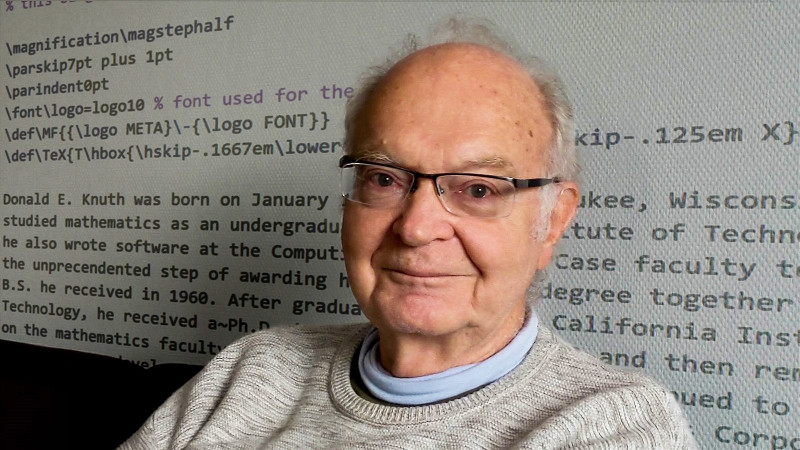
\includegraphics[width=0.5\linewidth,height=0.6\textheight,keepaspectratio]{figures/knuth.jpg}
\end{frame}
\note{
A partir da versão 3 o projeto foi congelado e só são lançadas correções de bugs. Os números das versões subsequentes aproximam assintóticamente $\pi$ (a versão atual, Março de 2008, é de número 3.1415926)

Knuth oferece um prêmio para quem encontrar Bug em seu código (valor inicial U\$2.56, dobrando a cada ano até atingir o valor atual U\$327.68)
}
\note{
When the first volume of Knuth's The Art of Computer Programming was published in 1969, it was typeset using hot metal type set by a Monotype Corporation typecaster with a hot metal typesetting machine from the 19th century which produced a "good classic style" appreciated by Knuth. When the second edition of the second volume was published, in 1976, the whole book had to be typeset again because the Monotype technology had been largely replaced by photographic techniques, and the original fonts were no longer available. However, when Knuth received the galley proofs of the new book on 30 March 1977, he found them awful. Around that time, Knuth saw for the first time the output of a high-quality digital typesetting system, and became interested in digital typography. The disappointing galley proofs gave him the final motivation to solve the problem at hand once and for all by designing his own typesetting system. On May 13, 1977, he wrote a memo to himself describing the basic features of TeX.
}
\note{
Even though Donald Knuth himself has suggested a few areas in which TeX could have been improved, he indicated that he firmly believes that having an unchanged system that will produce the same output now and in the future is more important than introducing new features. For this reason, he has stated that the "absolutely final change (to be made after my death)" will be to change the version number to $\pi$, at which point all remaining bugs will become features.
}


\begin{frame}
\frametitle{\LaTeX{}}


\includegraphics[width=0.5\linewidth]{figures/lion01.png}\hfill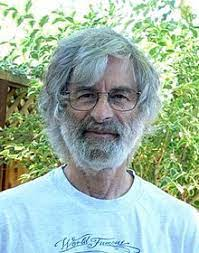
\includegraphics[width=0.15\linewidth]{figures/lamport.jpg}
\begin{itemize}
  \item \LaTeX{} (1984) é um conjunto de macros criado por Leslie Lamport utilizando comandos do \TeX{}.
  \item \LaTeX{} é uma linguagem de marcação e um sistema de preparação de documentos utilizando a formatação de texto do programa \TeX{} (para se escrever com \LaTeX{} adota-se uma abordagem diferente dos processadores de texto WYSIWYG).
  \item \TeX{} é um sistema de formatação de textos projetado com dois objetivos principais:
  \begin{enumerate}
      \item permitir que qualquer um possa produzir textos de \textbf{alta qualidade} com um esforço aceitável;
      \item fornecer um sistema que gere \textbf{exatamente o mesmo resultado} em todos os computadores, agora e no futuro.
  \end{enumerate}
\end{itemize}
\end{frame}



\begin{frame}
\frametitle{\TeX{}}
\framesubtitle{}
\centering{
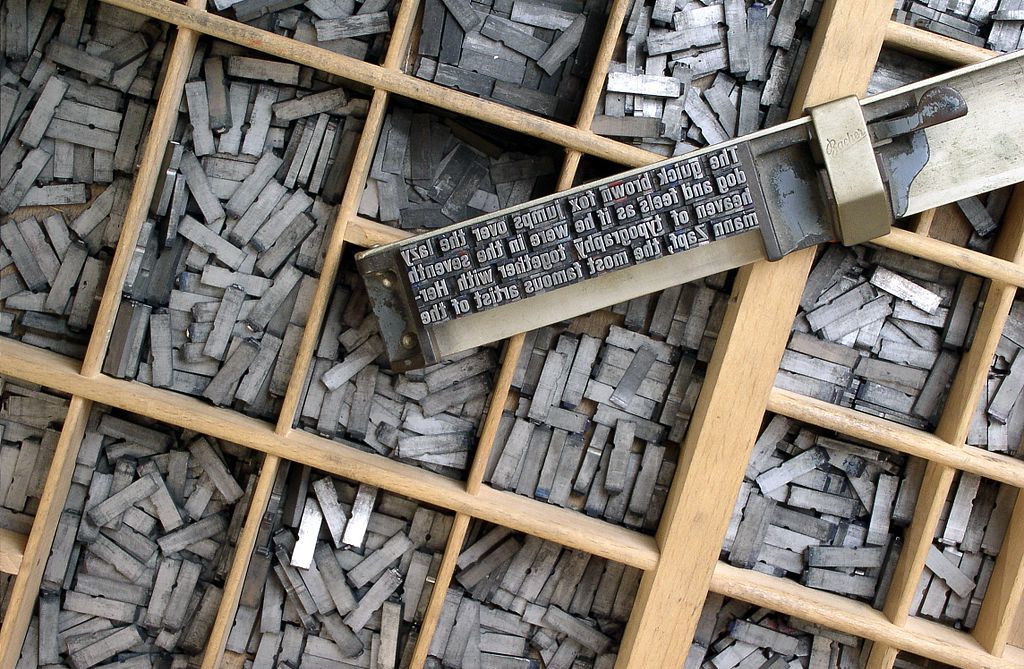
\includegraphics[width=0.6\linewidth,height=0.75\textheight,keepaspectratio]{figures/Metal_movable_type.jpg}
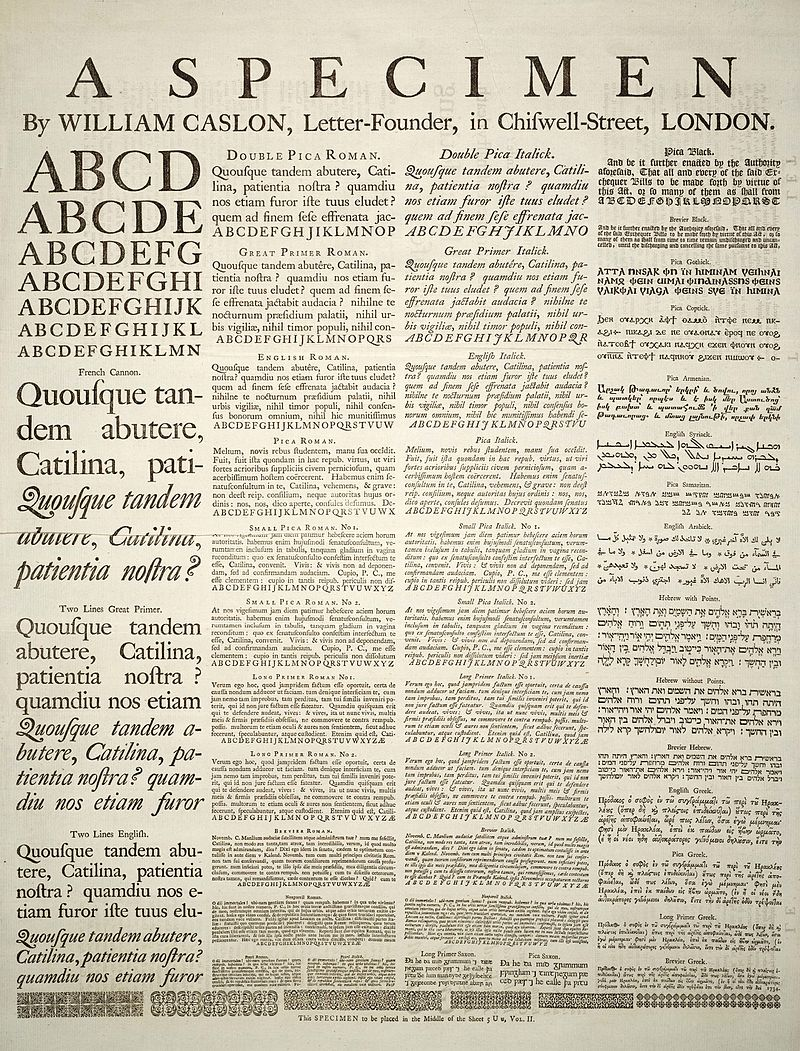
\includegraphics[width=0.3\linewidth,height=0.75\textheight,keepaspectratio]{figures/A_Specimen_by_William_Caslon.jpg}
}
\begin{flushleft}
\hspace{1.1em}\footnotesize{(Wikipedia)}
\end{flushleft}
\end{frame}
\note{
\TeX{} utiliza caixas (letras) e cola (espaços) para formar linhas palavras. 
Cada palavra é tratada como uma caixa e jutas formam linhas e parágrafos.
A cola é elastica e faz a separação entre as caixas, podendo comprimir ou exapandir.
}


\begin{frame}
\frametitle{\LaTeX{}}
\framesubtitle{}
\begin{itemize}
  \item \LaTeX{} é um conjunto de macros para o \TeX{} desenvolvido na década de 80 por Leslie Lamport.
  \item Amplamente utilizado no meio acadêmico, principalmente nas seguintes áreas: matemática, ciência da computação, engenharia, física, estatística e psicologia quantitativa.
\end{itemize}
\end{frame}



\begin{frame}
\frametitle{Licença}
\framesubtitle{}
\begin{itemize}
  \item \TeX{} possui licença de software permissiva (\hrefcolor{https://en.wikipedia.org/wiki/Comparison_of_free_and_open-source_software_licences}{BSD-like}).
  \item \LaTeX{} poussi licença própria: \LaTeX{} Project Public License (LPPL).
\end{itemize}
\end{frame}
\begin{frame}[allowframebreaks]
\frametitle{Por que utilizar \LaTeX{}?}
\framesubtitle{}
\begin{itemize}
  \item portabilidade - Linux, Mac OS, Windows, BSDs, Solaris, etc
  \item compatibilidade - padrão imutável
  \item flexibilidade
  \item controle
  \item apresentação e elegância nos documentos gerados
  \item facilidade em trocar estilos
  \item fórmulas matemáticas com alta qualidade
  \item tabelas, figuras
  \item disseminado (principalmente no meio acadêmico)
  \item estabilidade
  \item escalabilidade
  \item livre
  \item armazenamento de documentos de longo prazo (ASCII, UTF-8)
  \item controle de versão
  \item modularizar e colaborar documentos
  \item facilidade para lidar com documentos complexos
  \item bibliografia, índices e referências
\end{itemize}
\end{frame}


\begin{frame}
\frametitle{\LaTeX{} vs Word}
\framesubtitle{Devo utilizar \LaTeX{} ao invés do Word ou LibreOffice?}
  \begin{figure}[h!]
  \centering
  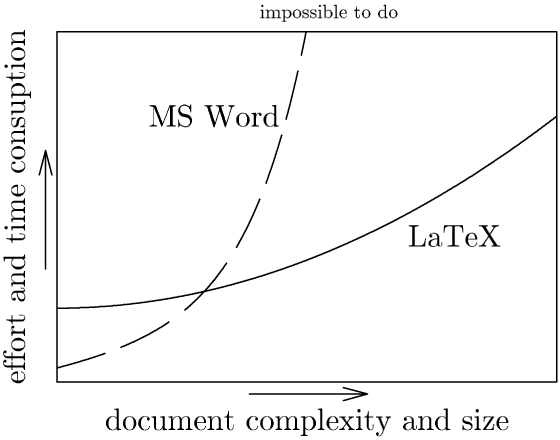
\includegraphics[width=0.5\textwidth]{figures/word_vs_latex.png}
  \caption{\LaTeX{} vs Word (John D. Cook).}
  \label{fig:word_vs_latex}
  \end{figure}
\end{frame}


\begin{frame}
\frametitle{Onde aprender \LaTeX{}?}
\begin{itemize}
  \item \hrefcolor{https://www.overleaf.com/learn/latex/Tutorials}{Tutorial Overleaf}
  \item \hrefcolor{https://en.wikibooks.org/wiki/LaTeX}{Wikibooks}
  \item \hrefcolor{https://drive.google.com/file/d/1ajERZETmHyAvp7Xa5j0pdFNjm4fNbmZY/view?usp=sharing}{\textcite{vivas_andrade_latex_2020}}
  \item \hrefcolor{http://www.ctan.org/tex-archive/info/lshort/english/lshort.pdf}{The Not So Short Introduction to LaTeX2e}
  \item \hrefcolor{https://books.google.com.br/books?id=iX9MAQAAQBAJ}{\textcite{goossens_latex_1993}}
  \item \hrefcolor{https://tex.stackexchange.com/}{StackExchange}
  \item Google Groups: \hrefcolor{https://groups.google.com/forum/\#!forum/comp.text.tex}{comp.text.tex}
  \item \LaTeX{} forum \hrefcolor{https://latex.org/forum/}{latex.org/forum/}
  \item \hrefcolor{https://www.latex-tutorial.com/}{\LaTeX{} Tutorial}
  \item \hrefcolor{http://www.ctan.org/}{CTAN} - documentações
  \item \hrefcolor{http://texample.net/}{texample}, \hrefcolor{https://texblog.org/}{texblog}
  \item Google
\end{itemize}
\end{frame}


\begin{frame}[fragile]
\frametitle{Como instalar o \LaTeX{}?}
\framesubtitle{}
\begin{itemize}
  \item \hrefcolor{http://www.tug.org/texlive/}{TeXLive} (GNU/Linux, Mac OS, Windows)
  \item \hrefcolor{http://www.miktex.org/}{MiKTeX} (GNU/Linux, Mac OS, Windows)
\end{itemize}
\vspace{3ex}

No Ubuntu, Debian ou demais distribuições da mesma família, basta usar o comando:
\begin{verbatim}
$ sudo apt-get install texlive
\end{verbatim}
\end{frame}



\begin{frame}
\frametitle{Editores para \LaTeX{}}
\framesubtitle{Até mesmo um bloco de notas pode ser um editor!}
\begin{itemize}
  \item \hrefcolor{http://www.xm1math.net/texmaker/}{TeXMaker} (cross-platform)
  \item \hrefcolor{http://kile.sourceforge.net/}{Kile} (KDE - Linux)
  \item \hrefcolor{http://www.lyx.org/}{Lyx} (versão WYSIWYM e cross-platform)
  \item \hrefcolor{https://www.texstudio.org/}{TeXstudio} (cross-platform)
  \item \hrefcolor{https://www.overleaf.com/}{Overleaf (ShareLaTeX + Overleaf)}
\end{itemize}
\end{frame}


\begin{frame}
\frametitle{Overleaf}
\framesubtitle{Editor online}
\begin{figure}
    \centering
    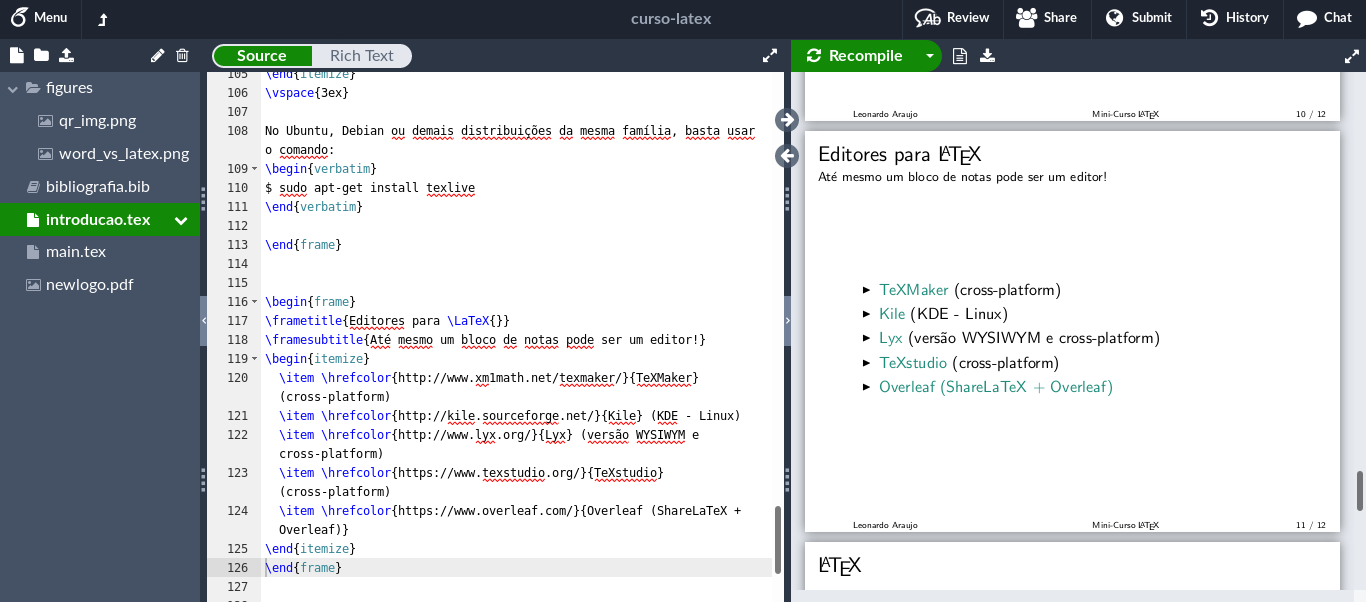
\includegraphics[width=\textwidth,height=0.7\textheight,keepaspectratio]{figures/overleaf.png}
    \caption{Editor online Overleaf.}
    \label{fig:overleaf}
\end{figure}
\end{frame}


\begin{frame}
\frametitle{Comparação entre editores}
\framesubtitle{Escolha a que mais lhe agrada!}
  \hrefcolor{http://en.wikipedia.org/wiki/Comparison_of_TeX_editors}{Comparação} entre editores \TeX \ na Wikipedia.

  \begin{figure}[h!]
  \centering
  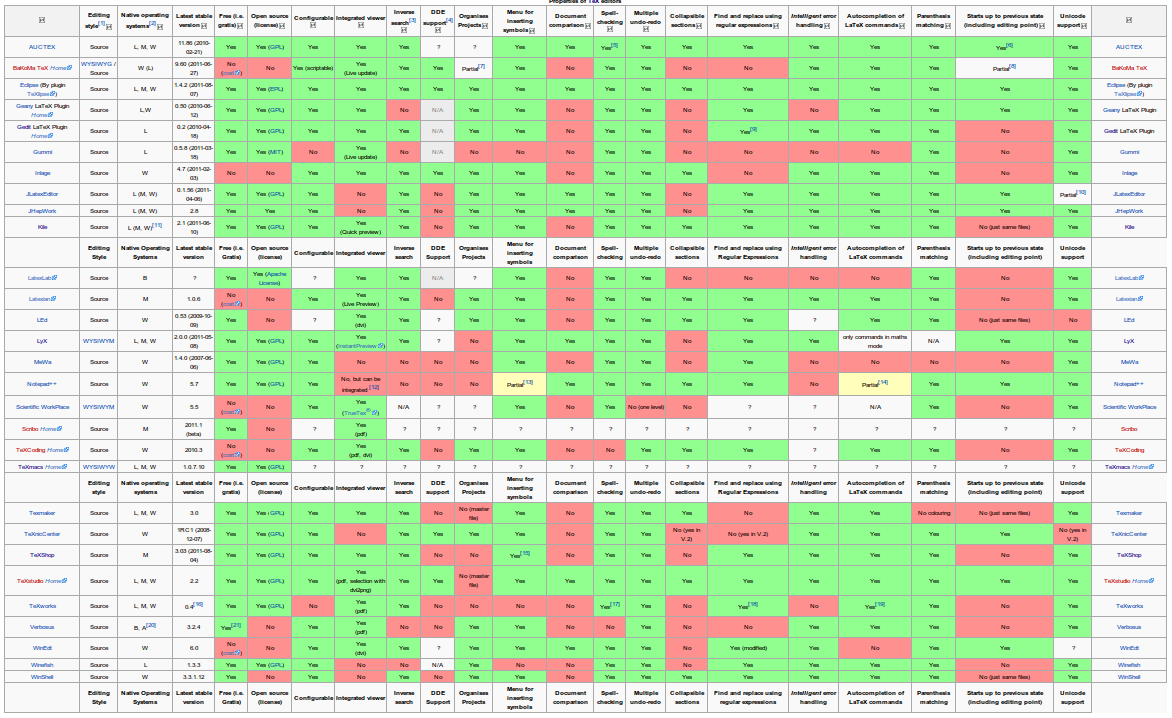
\includegraphics[width=0.8\textwidth,height=0.7\textheight,keepaspectratio]{figures/editorschart.png}
  \label{fig:editorschart}
  \end{figure}
\end{frame}


\begin{frame}
\frametitle{Compilando seu documento \TeX{}}
\framesubtitle{Para visualizar o documento é necessário compilá-lo.}
   \begin{description}
   \item[\TeX] gera um arquivo DVI (DeVice Independent) ao compilar um arquivo .tex
   \item[pdfTeX] gera um PDF
   \item[LaTeX2RTF] converter arquivo de \LaTeX (.tex) em um arquivo  Rich Text Format (.rtf)
   \item[dvips] converte um DVI em um aquivo PostScript (PS)
   \item[dvipdf] traduz um arquivo DVI em PDF
   \item[pdfLaTeX] gera um PDF diretamente
   \item[XeTeX] suporte a unicode
   \item[LuaTeX] linguagem de programação Lua
   \item[ConTeXt] interface simples para tipografia avançada
   \end{description}
\end{frame}




\section{Tipografia}
\begin{frame}
\frametitle{Escribas}
\begin{figure}[htbp]
\centering
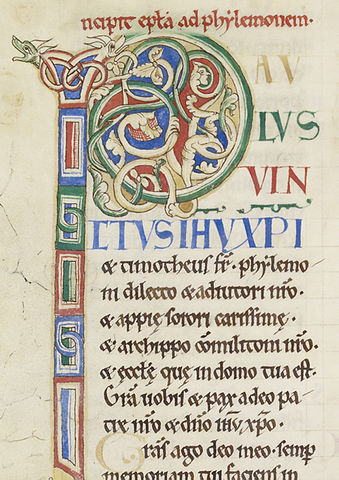
\includegraphics[width=0.35\textwidth,height=0.75\textheight,keepaspectratio]{figures/rochester_bible.jpg}
\caption{Primeira página da epístola de Paulo a Filêmon na Bíblia de Rochester (século 12).}
\label{fig-rochester_bible}
\end{figure}
\end{frame}
\note{
A preocupação com a estética dos textos é antiga.
Esta figura mostra um exemplos de escrita gótica utilizada pelos escribas nas cópias manuais que faziam 
do texto da bíblia.
É evidente a preocupação com a ornamentação e a elaboração de um visual rebuscado.

Quando Gutenberg criou os primeiros tipos móveis, para realizar cópias da bíblia, buscou ainda manter 
a escrita gótica.
}


\begin{frame}
\frametitle{Gutenberg}
\begin{figure}[htbp]
\begin{minipage}[t]{0.47\textwidth}
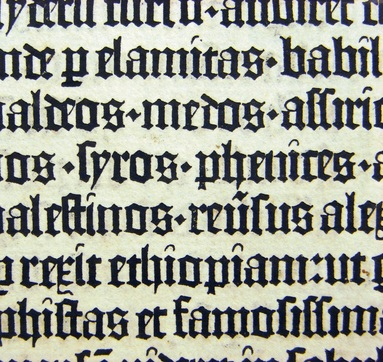
\includegraphics[width=0.8\linewidth,height=0.5\textheight,keepaspectratio]{figures/gutenberg.jpg}
\subcaption{Bíblia de Gutenberg.}
\end{minipage}
\hfill
\begin{minipage}[t]{0.47\textwidth}
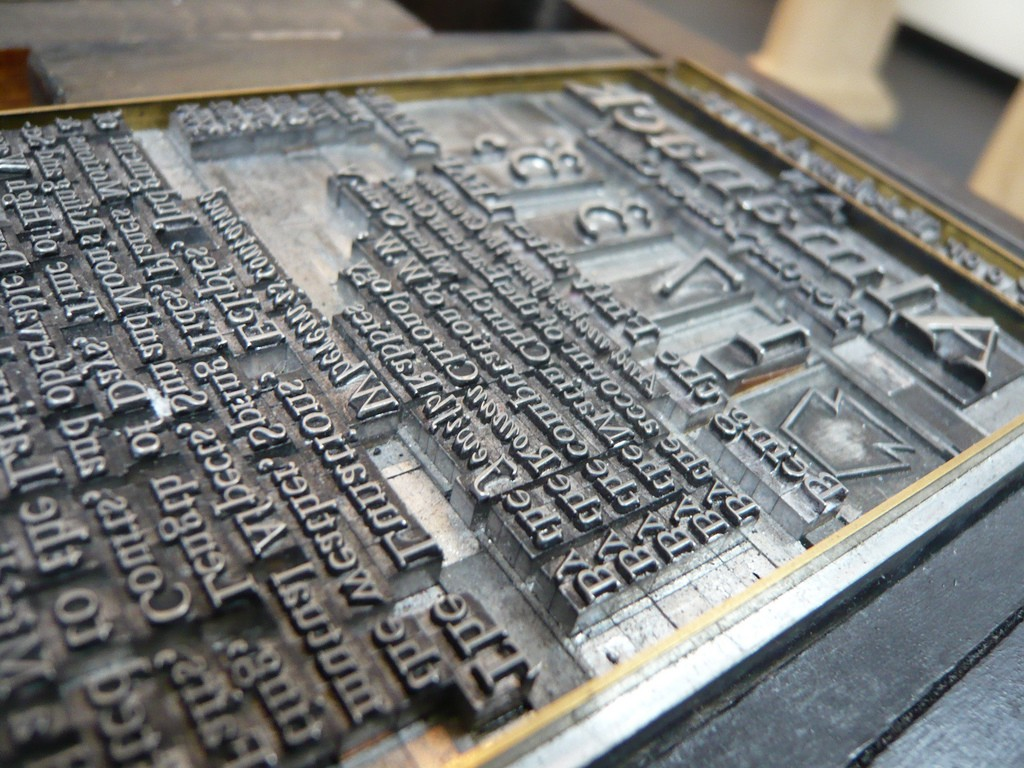
\includegraphics[width=\linewidth,height=0.5\textheight,keepaspectratio]{figures/mov-type.jpg}
\subcaption{Tipos móveis.}
\end{minipage}
\caption{Tipografia moderna.}
\end{figure}
\end{frame}

\begin{frame}[allowframebreaks]
\frametitle{A nova tipografia - Jan Tschichold, 1928}
\begin{figure}[htbp]
\centering
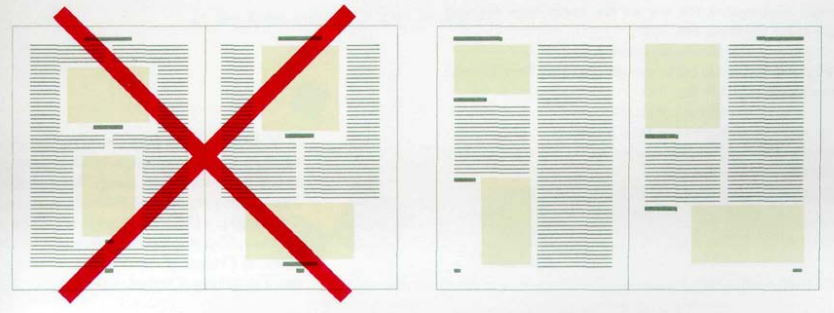
\includegraphics[width=\textwidth,height=0.5\textheight,keepaspectratio]{figures/jan-tschichold.png}
\caption{Comparação entre layouts.}
\label{fig-jan-tschichold}
\end{figure}

\begin{quote}
Trabalhar um texto de acordo com esses princípios geralmente resultará em um
ritmo diferente daquele da tipografia simétrica anterior. A assimetria é a
expressão rítmica do design funcional. Além de ser mais lógica, a assimetria
tem a vantagem de que sua aparência completa é muito mais eficaz opticamente do
que a simetria.
%Working through a text according to these principles will usually result in a
%rhythm different from that of former symmetrical typography. Asymmetry is the
%rhythmic expression of functional design. In addition to being more logical,
%asymmetry has the advantage that its complete appearance is far more optically
%effective than symmetry.
\end{quote}

\begin{quote} 
Daí o predomínio da assimetria na Nova Tipografia. Não menos importante, a
vivacidade da assimetria é também uma expressão de nosso próprio movimento e
este da vida moderna; é um símbolo das formas mutáveis da vida em geral, quando
o movimento assimétrico na tipografia toma o lugar do repouso simétrico. Este
movimento não deve, entretanto, degenerar em agitação ou caos. A busca pela
ordem também pode e deve ser expressa de forma assimétrica. É a única maneira
de tornar possível uma ordem melhor e mais natural, em oposição à forma
simétrica, que não extrai suas leis de dentro, mas de fora. 
%Hence the predominance of asymmetry in the New Typography. Not least, the
%liveliness of asymmetry is also an expression of our own movement and that of
%modern life; it is a symbol of the changing forms of life in general when
%asymmetrical movement in typography takes the place of symmetrical repose. This
%movement must not, however, degenerate into unrest or chaos. A striving for
%order can, and must, also be expressed in asymmetrical form. It is the only way
%to make a better, more natural order possible, as opposed to symmetrical form,
%which does not draw its laws from within itself but from outside.
\end{quote}

% https://readings.design/PDF/ThePrinciplesoftheNewTypography.pdf
% https://medium.com/@digitalonetwo/the-new-typography-excerpt-c2a3c1325f23
% https://www.fontfabric.com/blog/gutenberg-first-typeface-original-bible-typography-used/
\end{frame}


\begin{frame}
\frametitle{Recursos tipográficos}
O \TeX{} utiliza recursos tipográficos para melhorar a leitura e
a aparência (ou agradabilidade) dos textos.

Alguns deles são:
\begin{itemize}
  \item Ligadura
  \item Kerning
  \item Hifenização
  \item Quebra de linhas
  \item Justificação
  \item Quebra de parágrafos
  \item Controle de órfãos 
\end{itemize}
\end{frame}

\begin{frame}
\frametitle{\TeX{}}
\framesubtitle{Ligadura}

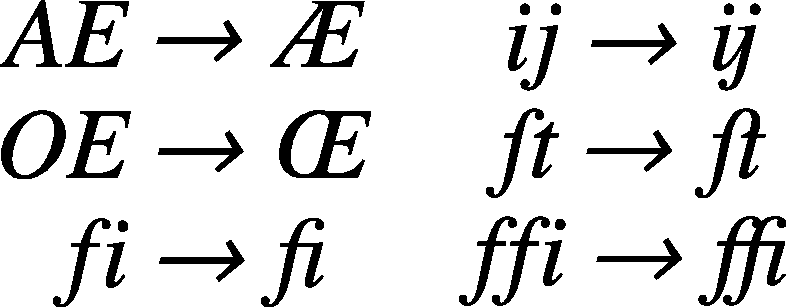
\includegraphics[width=0.35\linewidth]{figures/ligatures.pdf} \hspace{4em}
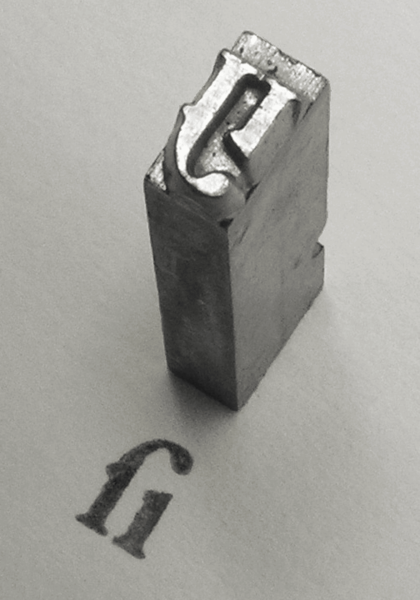
\includegraphics[width=0.15\linewidth]{figures/ligatures_fi.png}

\vspace{2ex}
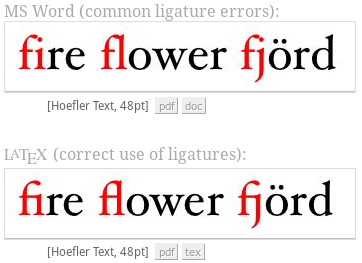
\includegraphics[width=0.3\linewidth]{figures/fire_ligatures.png}
\end{frame}


\begin{frame}
\frametitle{\TeX{}}
\framesubtitle{Kerning}
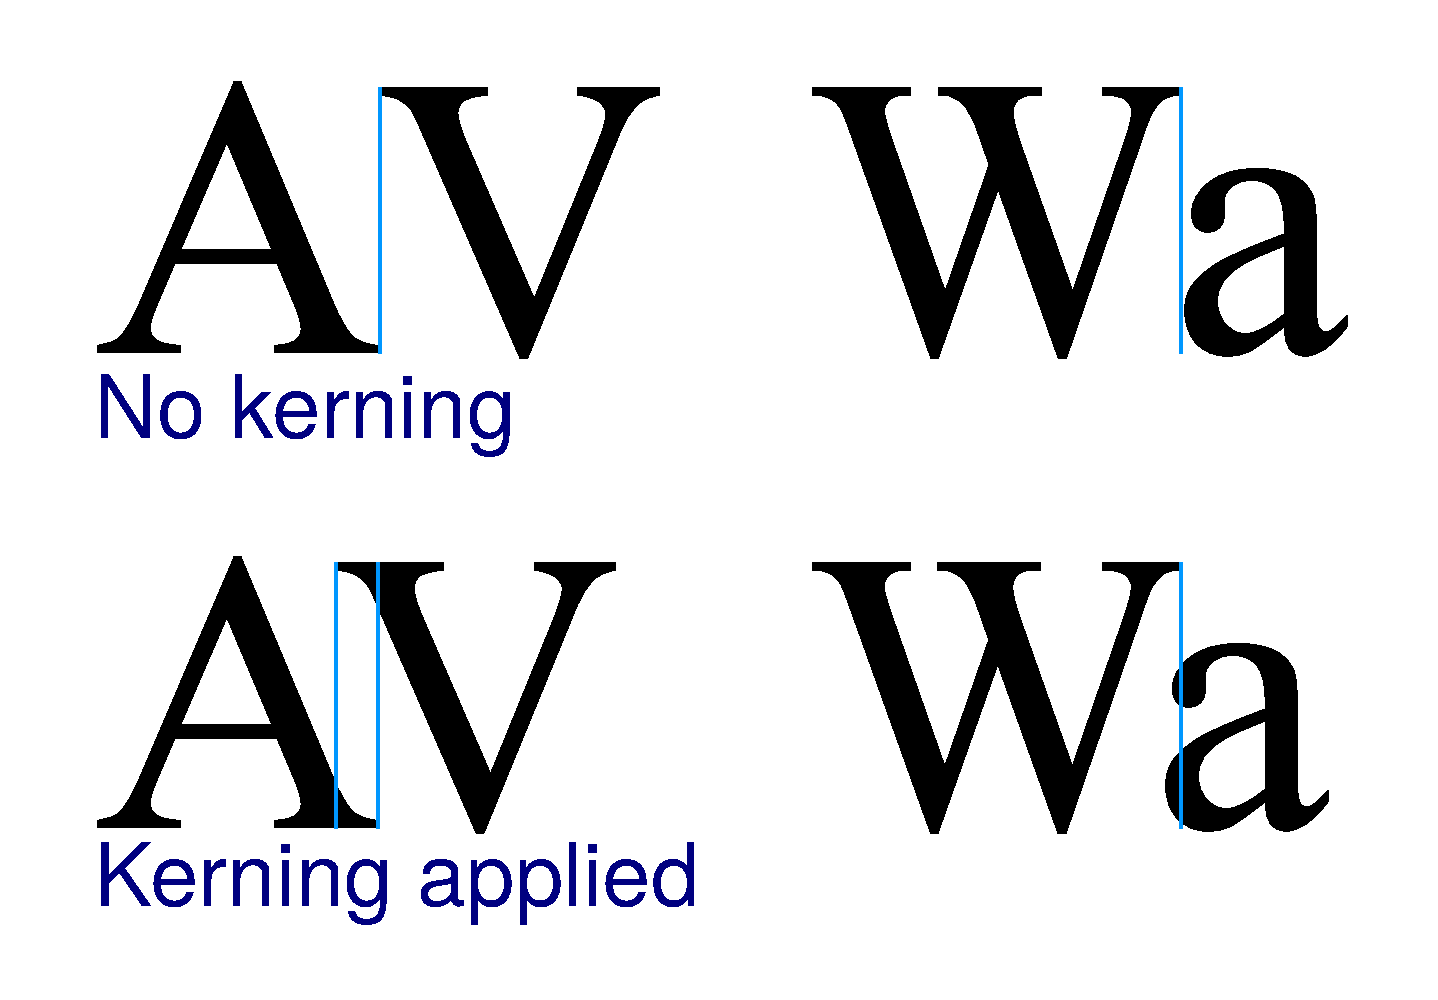
\includegraphics[width=0.3\linewidth]{figures/kerning.pdf}

\vspace{2ex}
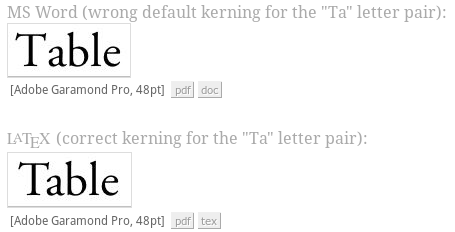
\includegraphics[width=0.4\linewidth]{figures/table_kerning.png}

\footnotesize{(Wikipedia, \url{http://nitens.org/taraborelli/latex})}
\end{frame}




\section{Documento \LaTeX{}}
\begin{frame}[fragile]
\frametitle{Estrutura de um documento em \LaTeX{}}
\begin{lstlisting}[language=tex, label=lst-estrutura, caption={Estrutura de um documento em \LaTeX{}}, postbreak=\mbox{$\hookrightarrow$\space}]
\documentclass{...}
...
\begin{document}
...
\end{document}
\end{lstlisting} %stopzone
\end{frame}

\begin{frame}[fragile]
\frametitle{Organização do texto em \LaTeX{}}
\begin{itemize}
\item título \verb|\title{...}|
\item autor \verb|\author{...}|
\item data \verb|\date{...}|
\item \verb|\maketitle|
\end{itemize}
\vspace{3ex}
\begin{itemize}
\item resumo \verb|\begin{abstract}...\end{abstract}|
\item capítulo \verb|\chapter{...}|
\item seções \verb|\section{...}|
\item subseções \verb|\section{...}|
\end{itemize}
\end{frame}

\begin{frame}[fragile]
\frametitle{Documento em \LaTeX{}}
\begin{lstlisting}[language=tex, label=lst-documento, caption={Exemplo de documento em \LaTeX{}}, postbreak=\mbox{$\hookrightarrow$\space}, basicstyle=\fontsize{8}{10}\selectfont\ttfamily]
\documentclass[10pt,a4paper]{article}
\usepackage[utf8]{inputenc}
\usepackage[T1]{fontenc}
\usepackage[portuguese]{babel}
\author{Leonardo}
\title{Meu primeiro artigo em \LaTeX{}}
\begin{document}
\maketitle
\begin{abstract}
Resumo do meu primeiro artigo em \LaTeX{}.
\end{abstract}
\section{Introdução}
Este exemplo ilustra um artigo simples em \LaTeX{}.
\section{Conclusão}
Fazer um artigo usando \LaTeX{} é simples!
\end{document}
\end{lstlisting} %stopzone
\end{frame}



\subsection{Exemplos}
\begin{frame}
\frametitle{Exemplos}
\framesubtitle{um documento simples}
  \begin{figure}[h!]
  \centering
  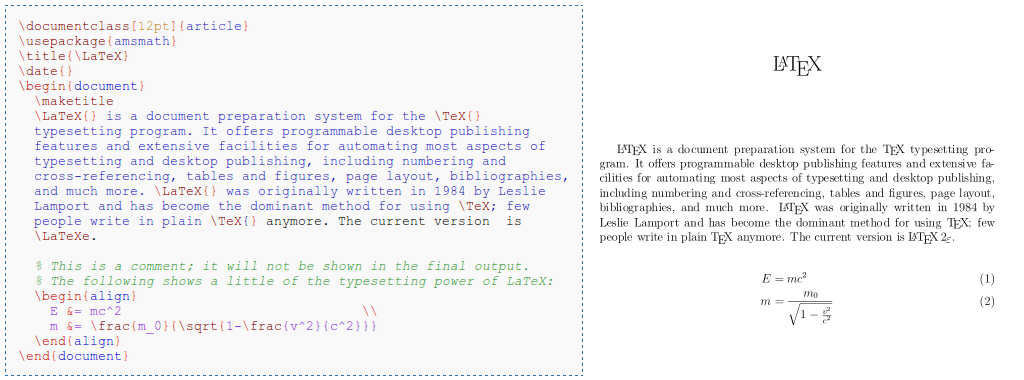
\includegraphics[width=\textwidth]{figures/exdoc.png}
  \label{fig:exdoc}
  \end{figure}
\end{frame}


\multido{\i=1+1}{7}{%
  \begin{frame}
    \frametitle{Exemplo}
    \framesubtitle{Abralin \i}
    \centering
    \includegraphics[height=0.7\textheight]{figures/abralin0\i.png}
  \end{frame}
 }
 
\multido{\i=1+1}{4}{%
  \begin{frame}
    \frametitle{Exemplo}
    \framesubtitle{\hrefcolor{https://www.tug.org/texshowcase/}{TeX showcase} \i}
    \centering
    \includegraphics[width=0.7\linewidth,height=0.7\textheight,keepaspectratio]{figures/showcase0\i.png}
  \end{frame}
 }




\begin{frame}
Sugestões de leitura: 
\vspace{2ex}

\fullcite{knuth_texbook_1984}
\vspace{2ex}

\fullcite{lamport_latex_1994}
\vspace{2ex}

\fullcite{wikibook}
\vspace{2ex}

\fullcite{vivas_andrade_latex_2020}
\end{frame}


\begin{frame}
\frametitle{Aprendendo \LaTeX{}}
\framesubtitle{}
\centering
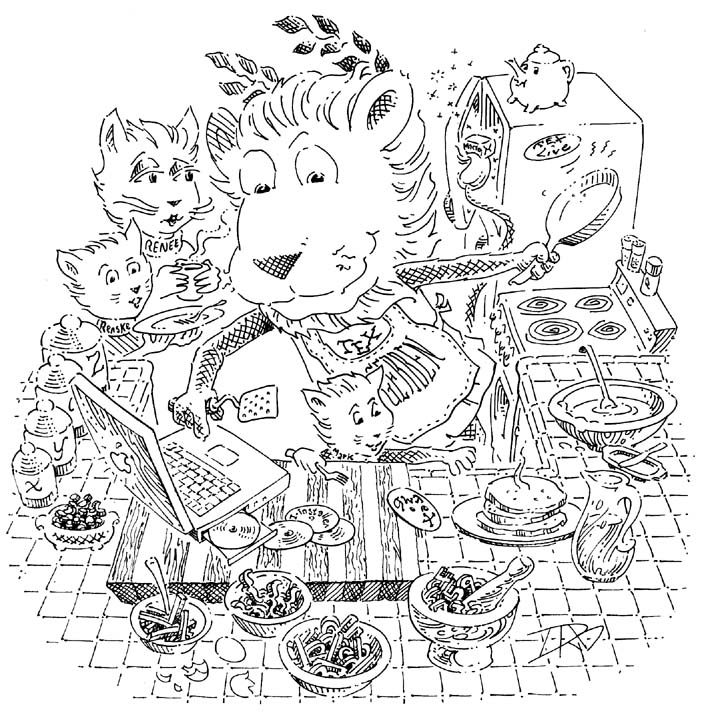
\includegraphics[width=0.6\linewidth,height=0.7\textheight,keepaspectratio]{figures/lion02.png}
\end{frame}

\begin{frame}
\frametitle{Arquivos}
\framesubtitle{Quais arquivos são utilizados?}
\begin{description}
\item[.tex] arquivo fonte do documento \TeX{} ou \LaTeX{}
\item[.cls] arquivo de classe de documento
\item[.sty] arquivo de estilo, pacotes 
\item[.bib] arquivo de bibliografia do BibTeX
\end{description}
\end{frame}

\begin{frame}
\frametitle{Conteúdo e Apresentação}
\framesubtitle{foque em uma coisa de cada vez e diminua o esforço necessário}
  CSS/HTML (web design) e \LaTeX{} (formatação de texto) são exemplos onde empregamos a separação entre conteúdo e forma.
  \begin{figure}[h!]
  \centering
  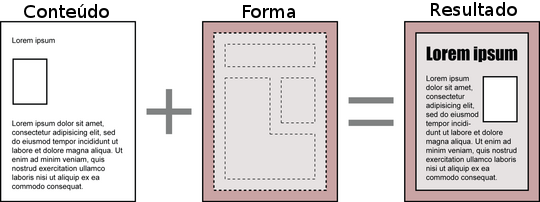
\includegraphics[width=0.7\textwidth,height=0.7\textheight,keepaspectratio]{figures/content_design.png}
  \label{fig:content_design}
  \end{figure}
\end{frame}



\subsection{Arquivo \TeX{}}\label{sec:tex}
\begin{frame}
\frametitle{Arquivo .tex}
\framesubtitle{principal arquivo do seu documento}
O arquivo .tex será o principal arquivo do seu documento. Neste arquivo você incluirá/definirá:
\begin{itemize}
    \item classe do documento
    \item tamanho de fonte, tamanho da página, coluna simples ou dupla, etc
    \item pacotes
    \item texto, figuras, tabelas, equações
    \item outros arquivos .tex
    \item bibliografia
\end{itemize}
\end{frame}


\begin{frame}[fragile]
\frametitle{Espaços em branco}
\framesubtitle{}
  Um ou vários espaços em branco são tratados como um único espaço em branco.
\begin{LTXexample}
Não interessa se introduz apenas
um ou vários     espaços depois
de uma palavra.

Uma linha em branco inicia um novo
parágrafo. 
\end{LTXexample}
\end{frame}


\begin{frame}[fragile]
\frametitle{Caracteres reservados}
\framesubtitle{}
Alguns caracteres são reservados:
\begin{verbatim}
#  $  %  ^  &  _  {  }  ~  \ 
\end{verbatim}

Para escrever um desses caracteres é necessário utilizar o caractere de escape.
  \vspace{1cm}
\begin{LTXexample}[commentstyle=\color{black}]
  \# \$ \% \^{} \& \_ \{ \} \~{} \textbackslash
\end{LTXexample}
\end{frame}


\begin{frame}[fragile]
\frametitle{Comandos}
\framesubtitle{}
Começam com um backslash e têm um nome que consiste apenas de letras. Os comandos obedecem à seguinte sintaxe:

\begin{verbatim}
\commandname[option1,option2,...]{argument1}{argument2}...
\end{verbatim}

\begin{LTXexample}
Li que o Knuth divide as
pessoas que trabalham com o \TeX{}
em \TeX{}nicos e \TeX pertos.\\
Hoje é \today.
\end{LTXexample}
\end{frame}


\begin{frame}[fragile]
\frametitle{Ambientes}
Os ambientes são utilizados para formatar blocos de texto em \LaTeX{}.
Os ambientes possuem a seguinte sintaxe:

\begin{verbatim}
\begin{environment_name}{arguments}[optional_arguments]
...
\end{environment_name}
\end{verbatim}

\begin{LTXexample}
\begin{center}
\lipsum[1][1-4]
\end{center}
\end{LTXexample}

\end{frame}


\begin{frame}[fragile]
\frametitle{Comentários}
\framesubtitle{}
Tudo o que vem após o carácter \% é um comentário. Podemos também fazer comentários em bloco.

\begin{LTXexample}
Este é um % estúpido
% Melhor: instrutivo <----
exemplo: Supercal%
ifragilist%
icexpialidocious

Este é outro
\begin{comment}
bastante estúpido,
mas instrutivo
\end{comment}
exemplo de como embeber
comentários nos seus documentos.
\end{LTXexample}:
\end{frame}

\begin{frame}[fragile]
\frametitle{Estrutura}
\framesubtitle{}
  A seguinte estrutura é esperada em um arquivo \LaTeX{}.

\begin{verbatim}
\documentclass{...}
\usepackage{...}
...
\begin{document}
...
\end{document}
\end{verbatim}
\end{frame}

\begin{frame}[fragile]
\frametitle{Exemplo}
\framesubtitle{}
  \scriptsize
  \begin{columns}[c]
  \column{.5\textwidth}
  \begin{figure}[h!]
  \centering
  \setlength\fboxsep{0pt}
  \setlength\fboxrule{0.5pt}
  \fbox{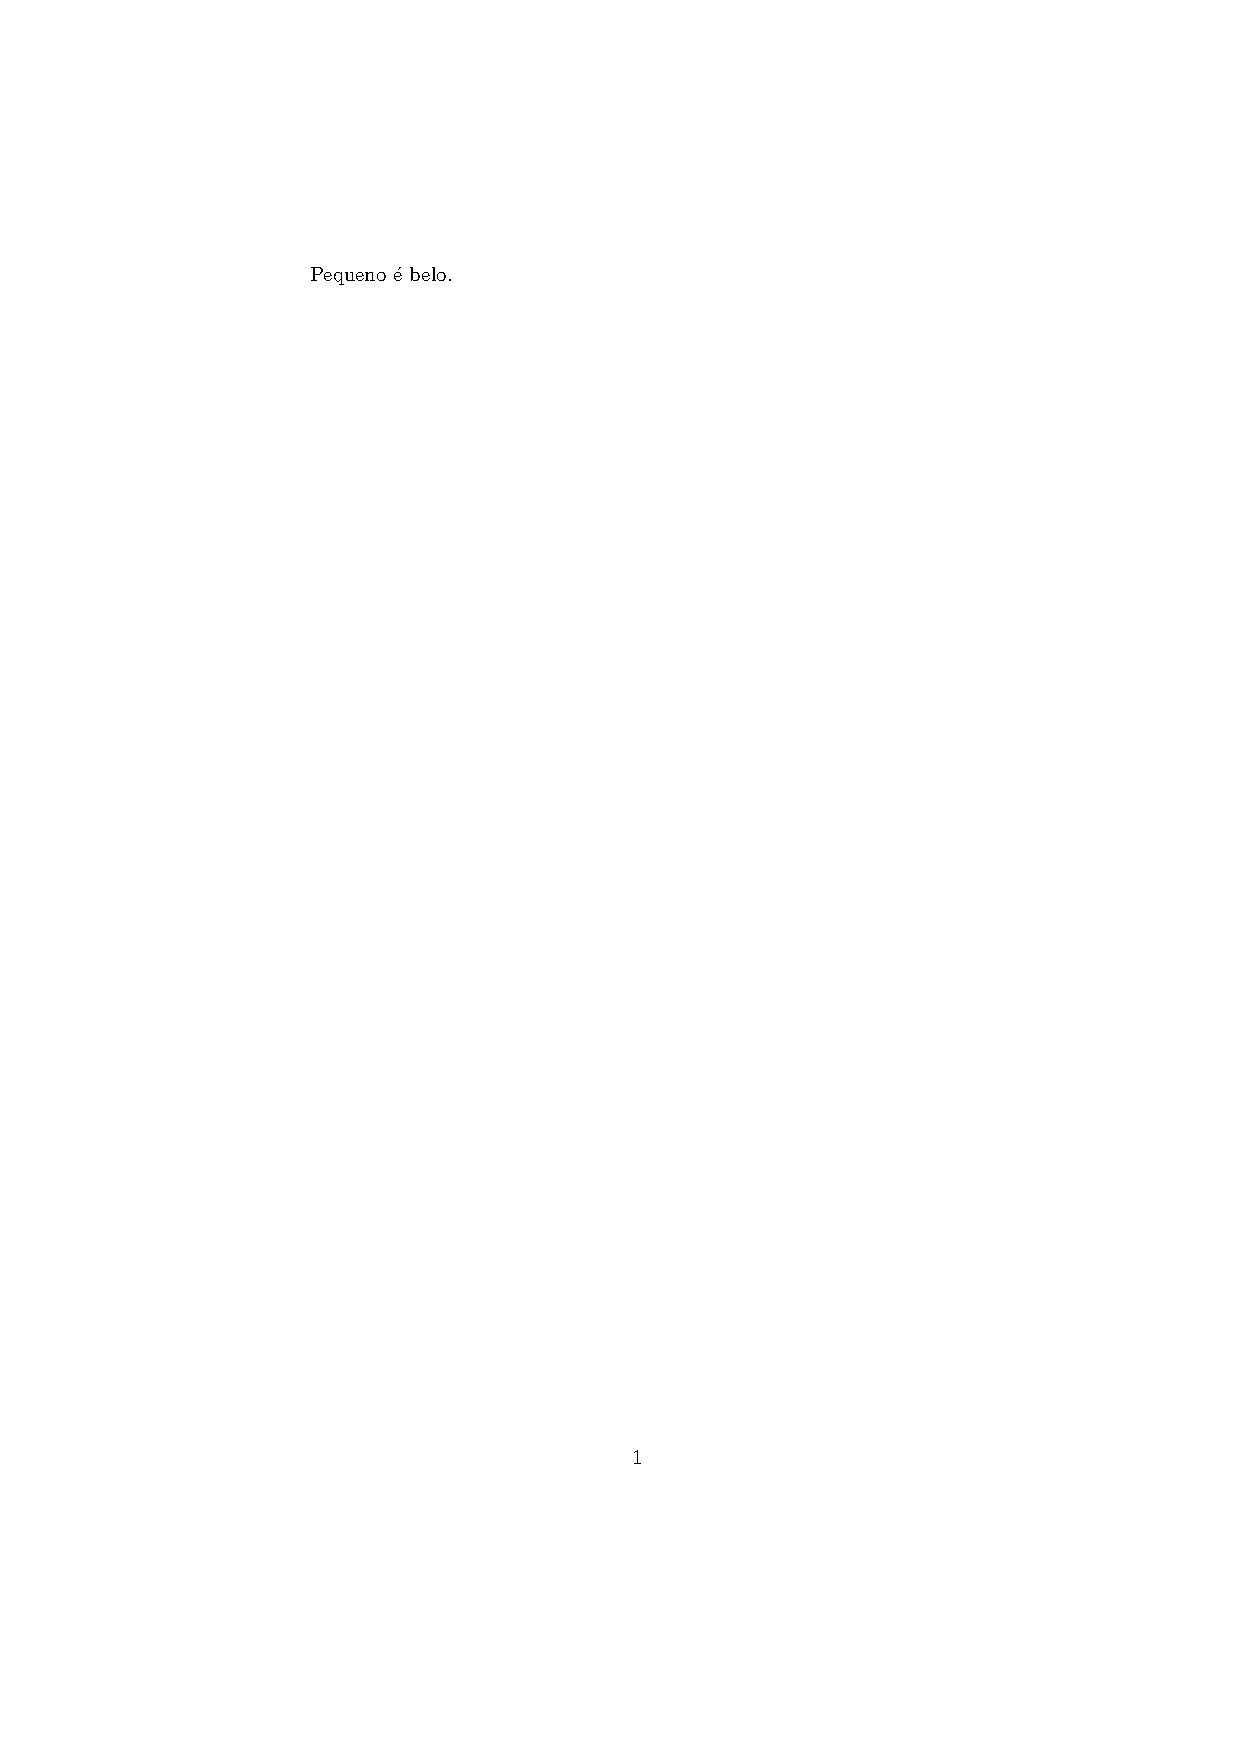
\includegraphics[width=0.7\textwidth,height=0.8\textheight,keepaspectratio]{minimal.pdf}}
  \label{fig:minimal}
  \end{figure}
  \column{.5\textwidth}
  \begin{verbatim}
\documentclass{article}
% esta linha é específica para
% o Português e outras línguas
% com caracteres acentuados.
\usepackage[latin1]{inputenc}
\begin{document}
Pequeno é belo.
\end{document}
\end{verbatim}
  \end{columns}
\end{frame}

\begin{frame}[fragile]
\frametitle{Exemplo 2}
\framesubtitle{}
  \scriptsize
  \begin{columns}[c]
  \column{.5\textwidth}
  \begin{figure}[h!]
  \centering
  \setlength\fboxsep{0pt}
  \setlength\fboxrule{0.5pt}
  \fbox{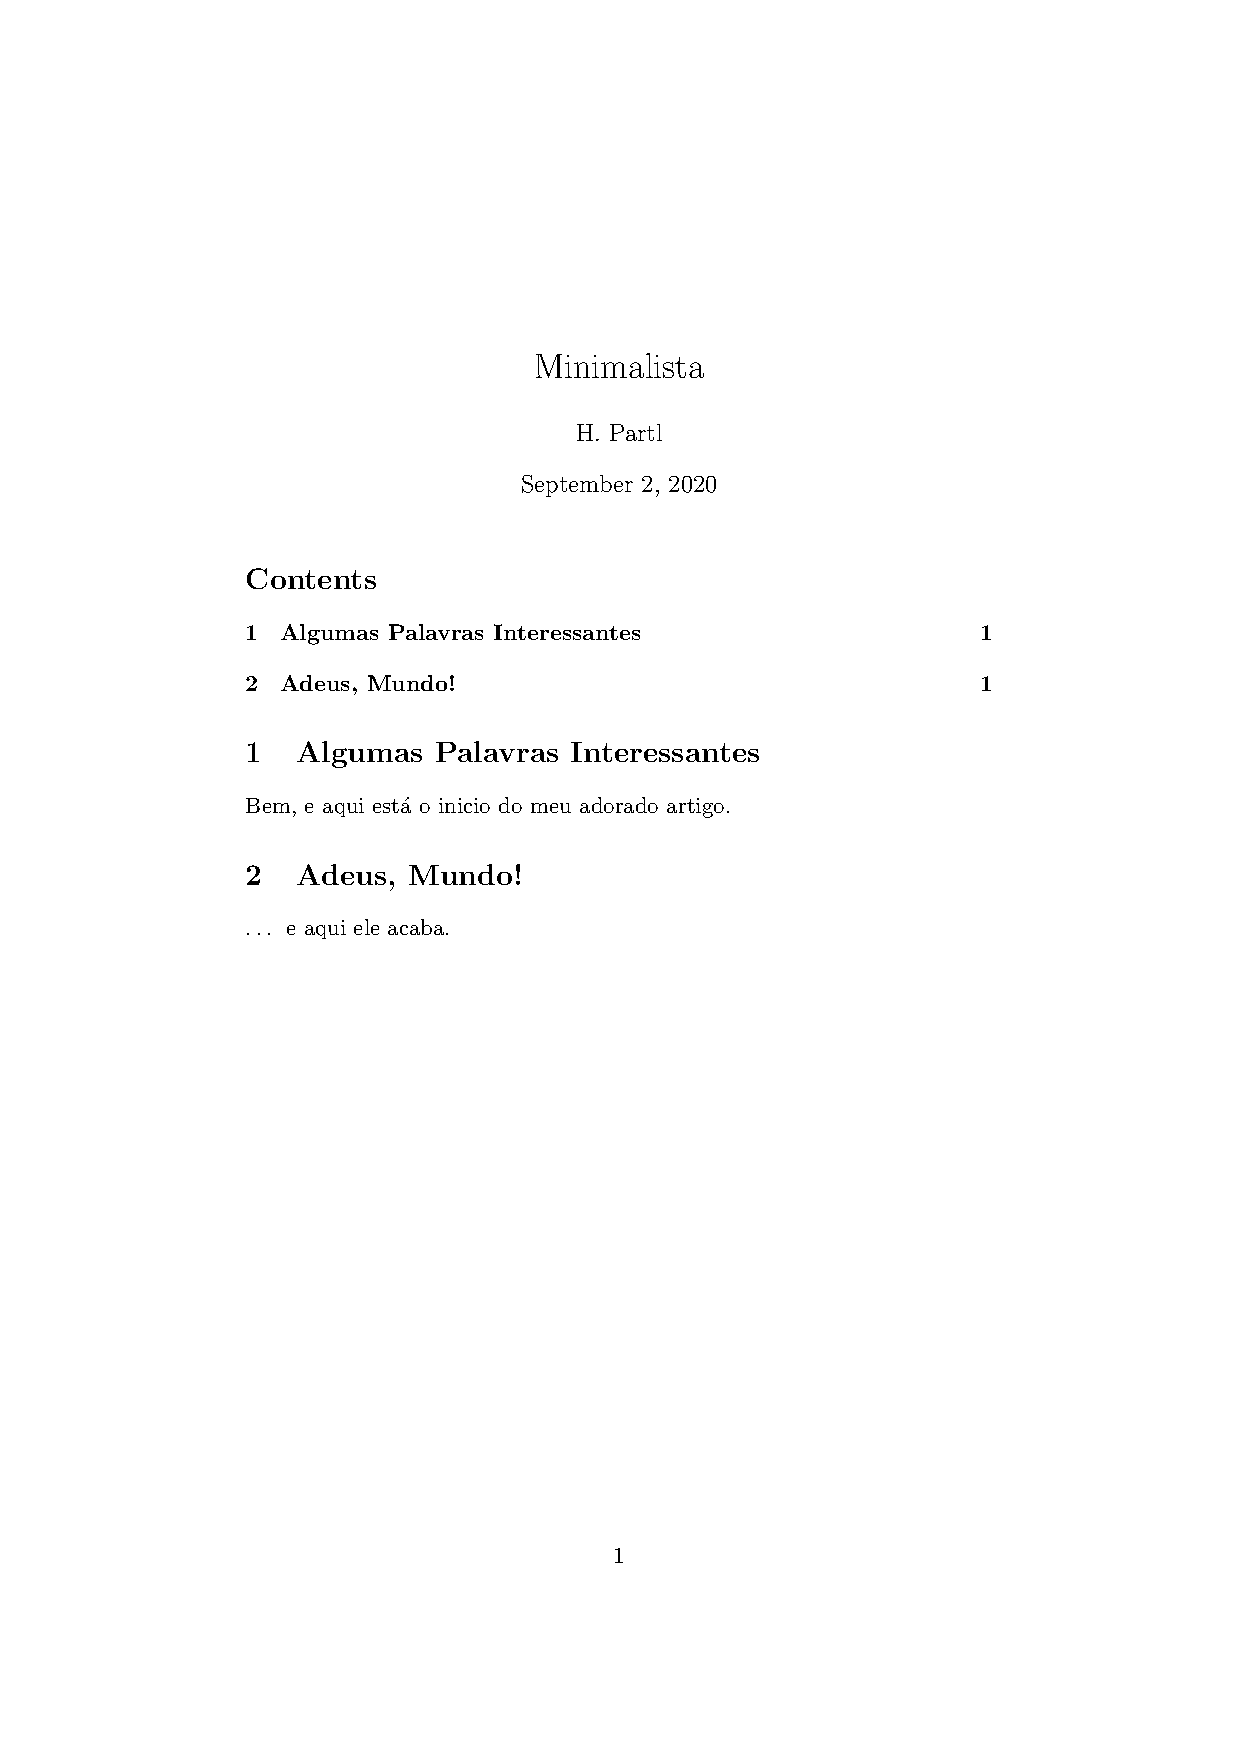
\includegraphics[width=0.7\textwidth,height=0.8\textheight,keepaspectratio]{minimal2.pdf}}
  \label{fig:minimal2}
  \end{figure}
  \column{.5\textwidth}
\begin{verbatim}
\documentclass[a4paper,11pt]{article}
% Esta linha é necessária para
% documentos em línguas que incluam
% caracteres acentuados.
\usepackage[latin1]{inputenc}
% Define o autor e título
\author{H.Partl}
\title{Minimalista}
\begin{document}
% Gera o título
\maketitle
% Insere a tabela de conteúdos
\tableofcontents
\section{Algumas Palavras Interessantes}
Bem, e aqui está o inicio do meu adorado artigo.
\section{Adeus, Mundo!}
\ldots{} e aqui ele acaba.
\end{document}
\end{verbatim}
  \end{columns}
\end{frame}


\subsection{Classes}
\begin{frame}[fragile,allowframebreaks]
\frametitle{Documento}
\framesubtitle{classes de documento}
  \begin{verbatim}
  \documentclass[opções]{classe}
  \end{verbatim}
  Exemplo:
  \begin{verbatim}
  \documentclass[11pt,twoside,a4paper]{article}
  \end{verbatim}

  Classes
  \begin{description}
  \item[article] para artigos em jornais científicos, pequenos relatórios, documentação de programas, convites, ...
  \item[report] para relatórios mais longos contendo vários capítulos, pequenos livros, teses de doutorado, ...  
  \item[book] para livros
  \item[slides] para slides. Esta classe usa letras grandes do tipo sans serif. Deve-se
       considerar utilizar o pacote Beamer.
  \end{description}

  \framebreak
  Pacotes de classes:
  \begin{itemize}
  \item \hrefcolor{https://ctan.org/pkg/koma-script}{KOMA-Script} fornece as seguintes classes: \emph{article}, \emph{report}, \emph{book} e \emph{letter}.
    As classes do KOMA-Script seguem o estilo dado pelo tipógrafo Jan Tschichold.
  \item \hrefcolor{https://www.ctan.org/pkg/memoir}{memoir} fornece classes para poesias, trabalhos matemáticos, obras ficcionais e não ficcionais.
  \item \hrefcolor{https://ctan.org/pkg/beamer}{beamer} é uma classe para apresentações em slides.
  \item \hrefcolor{https://ctan.org/pkg/sciposter}{sciposter} é uma classe para posters científicos.
  \end{itemize}

\end{frame}

\begin{frame}
\frametitle{Classes}
\framesubtitle{atributos das classes}
  Opções:

  \begin{description}[a4paper, b5paper, letterpaper]
  \item[10pt, 11pt, 12pt] para definir o tamanho da fonte
  \item[a4paper, b5paper, letterpaper] para definir o tamanho do papel
  \item[titlepage, notitlepage] especifica se se deve criar uma nova página depois do título do documento ou não
  \item[twocolumn, onecolumn] documento em duas colunas
  \item[twoside, oneside] impressão frente-verso ou não  
  \item[openright, openany] faz os capítulos começarem apenas nas páginas do lado direito ou na próxima disponível
  \item[landscape] formato paisagem
  \item[outras] depende de cada classe
  \end{description}
\end{frame}



\begin{frame}[label={clsfile}]
\frametitle{Arquivo de classe de documento, arquivo de estilo e pacote}
\framesubtitle{.cls e .sty}
Qualquer um pode definir sua própria classe.

\vspace{6ex}
Veja o tutorial no  \hrefcolor{https://www.overleaf.com/learn/latex/Understanding_packages_and_class_files}{Overleaf}
\end{frame}



\subsection{Documento .tex}
\begin{frame}[fragile]
\frametitle{Documento}
\framesubtitle{Incluir um documento em outro documento}
  Pomos incluir um arquivo \texttt{.tex} dentro de outro. Para tanto, basta fazer:
  
  \begin{verbatim}
  \input{nome_do_arquivo}
  
  \include{nome_do_arquivo} 
  equivalente a 
  \clearpage \input{nome_do_arquivo} \clearpage
  \end{verbatim}
\end{frame}



\begin{frame}[fragile]
\frametitle{Documento}
\framesubtitle{Comandos de Secção}
  
\begin{verbatim}
\part{}

\chapter{}

\section{}

\subsection{}

\subsubsection{}

\paragraph{}
\end{verbatim}

\end{frame}



\begin{frame}[fragile]
\frametitle{Documento}
\framesubtitle{quebra de linha e nova página}
\begin{LTXexample}
  você pode \\ quebrar uma linha 
  quando quiser no \newline \LaTeX, 
  entretanto uma simples quebra
  de linha do código não reflete 
  em quebra de linha... 
  
  mas você pode deixar uma linha 
  em branco
\end{LTXexample}  
  Comando utilizado para iniciar uma nova página: \verb|\newpage|
\end{frame}


\begin{frame}[fragile]
\frametitle{Documento}
\framesubtitle{Hifenização de palavras}
  \begin{verbatim}
\hyphenation{lista de palavras}
  \end{verbatim}

\begin{LTXexample}
  \hyphenation{MINICURSOLATEX uni-ver-si-da-de}
  Penso que isto é: su\-per\-cal\-%
  i\-frag\-i\-lis\-tic\-ex\-pi\-%
  al\-i\-do\-cious
  
  Teste de hifenização da palavra 
  universidade, inclusive de  
  certa  palavra MINICURSOLATEX, 
  que não deve ser hifenizada.
\end{LTXexample}
\end{frame}


\begin{frame}[fragile]
\frametitle{Documento}
\framesubtitle{Estilo de fonte em um texto}
\begin{LTXexample}
  \textbf{Bold} \\
  \textit{Italic} \\
  \texttt{Monotype} \\
  \textsf{Sans Serif} \\
  \textsc{SmallCaps} \\
  \textsl{Slanted} \\
  \emph{Enfase}
\end{LTXexample}
\end{frame}


\begin{frame}[fragile]
\frametitle{Documento}
\framesubtitle{Tamanho da fonte em um texto}
\begin{LTXexample}
  {\tiny texto texto ...} \\
  {\scriptsize texto texto ...} \\
  {\footnotesize texto texto ...} \\
  {\small texto texto ...} \\
  {\normalsize texto texto ...} \\
  {\large texto texto ...} \\
  {\Large texto texto ...} \\
  {\LARGE texto texto ...} \\
  {\huge texto texto ...} \\
  {\Huge texto texto ...}
\end{LTXexample}
\end{frame}

\begin{frame}[fragile]
\frametitle{Documento}
\framesubtitle{Alinhamento de texto}
\begin{LTXexample}
  \begin{center}
  texto texto
  \end{center}
  \begin{flushleft}
  texto texto
  \end{flushleft}
  \begin{flushright}
  texto texto
  \end{flushright}
\end{LTXexample}
\end{frame}

\begin{frame}[fragile]
\frametitle{Documento}
\framesubtitle{Layout de uma página}
  \scriptsize
  \begin{columns}[c]
  \column{.5\textwidth}
  \begin{itemize}
  \item \verb|\hoffset|
  \item \verb|\voffset|
  \item \verb|\oddsidemargin|
  \item \verb|\topmargin|
  \item \verb|\headheight|
  \item \verb|\headsep|
  \item \verb|\textheight| 
  \item \verb|\textwidth|
  \item \verb|\marginparsep|
  \item \verb|\marginparwidth|
  \item \verb|\footskip|
  \end{itemize}
  \column{.5\textwidth}
  \vspace{-1.5cm}
\begin{figure}[h!]
  \centering
  \label{fig:Latex_layout}
    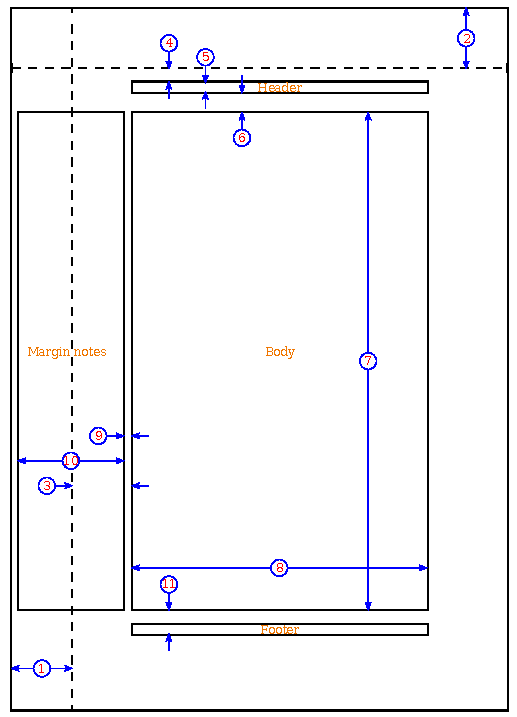
\includegraphics[width=0.8\textwidth,height=.95\textheight,keepaspectratio]{figures/Latex_layout.pdf}
  %\caption{Tux.}
\end{figure}
  \end{columns}
\end{frame}


\begin{frame}[fragile]
\frametitle{Documento}
\framesubtitle{Layout}
  \begin{verbatim}
\documentclass[a4paper]{article}
\usepackage[top=tlength, bottom=blength, left=llength,
        right=rlength]{geometry}
\usepackage[a4paper,landscape]{geometry}
  \end{verbatim} 
\end{frame}


\begin{frame}[fragile]
\frametitle{Documento}
\framesubtitle{Cabeçalho e Rodapé}
  \begin{verbatim}
\usepackage{fancyhdr}

\fancyhead[CE]{Author's Name}
\fancyhead[CO]{\today}
\fancyfoot[LE,RO]{\thepage}
  \end{verbatim} 
  
  \url{https://ctan.org/pkg/fancyhdr} \\
  \url{https://www.overleaf.com/learn/latex/Headers_and_footers}
\end{frame}


\begin{frame}[fragile]
\frametitle{Documento}
\framesubtitle{misturar coluna simples com multiplas colunas}

\small
\begin{LTXexample}
\lipsum[1][1-2]
\begin{multicols}{2}
\lipsum[1][3-6]
\end{multicols}
\lipsum[1][7-9]
\end{LTXexample}

\url{https://www.ctan.org/pkg/multicol} \\
\url{https://www.overleaf.com/learn/latex/Multiple_columns}
\end{frame}


\begin{frame}[fragile]
\frametitle{Documento}
\framesubtitle{Notas de rodapé}
\begin{LTXexample}
No meio do texto, podemos colocar a nota de rodapé\footnote{Nota que fica na
parte inferior da página.} para explicações adicionais tais como significado da
palavra, ou fonte que foi usada.
\end{LTXexample}
No meio do texto, podemos colocar a nota de rodapé\footnote{Nota que fica na
parte inferior da página.} para explicações adicionais tais como significado da
palavra, ou fonte que foi usada.
\end{frame}

\begin{frame}[fragile]
\frametitle{Documento}
\framesubtitle{Sumário}
\begin{LTXexample}
\tableofcontents
\end{LTXexample}
\end{frame}


\begin{frame}[fragile]
\frametitle{Documento}
\framesubtitle{Sumário - local corrente}
\begin{LTXexample}
\tableofcontents[current,currentsection]
\end{LTXexample}
\end{frame}


%\subsection{Linguística}\label{sec:linguistica}
%\section{Linguística}

\begin{frame}[fragile]
\frametitle{Linguística}
\framesubtitle{Ferramentas para trabalhos em linguística}

\begin{enumerate}
    \item caracteres IPA
    \item árvores sintáticas
    \item árvores de dependências
    \item exemplos enumerados
\end{enumerate}

\end{frame}


\begin{frame}[fragile]
\frametitle{Linguística}
\framesubtitle{escrita fonética}
  \scriptsize
  \begin{columns}[c]
  \column{.5\textwidth}
  \begin{verbatim}
   \usepackage{tipa}
   
   \textipa{abcdefghijklmnopqrstuvwxyz}
   \textipa{ABCDEFGHIJKLMNOPQRSTUVWXYZ}
   \textipa{1234567890 @}
   \textipa{\:d \:l \:n \:r \:s \:t \:z}
   \textipa{\!b \!d \!g \!j \!G \!o}
  \end{verbatim}
  \column{.5\textwidth}
  \begin{fmpage}{\textwidth}
   \textipa{abcdefghijklmnopqrstuvwxyz}
   \textipa{ABCDEFGHIJKLMNOPQRSTUVWXYZ}
   \textipa{1234567890 @}
   \textipa{\:d \:l \:n \:r \:s \:t \:z}
   \textipa{\!b \!d \!g \!j \!G \!o}
  \end{fmpage}
  \end{columns}

  \url{https://www.tug.org/TUGboat/tb17-2/tb51rei.pdf}
  \url{https://ctan.org/pkg/tipa}

\end{frame}


\begin{frame}[fragile]
\frametitle{Linguística}
\framesubtitle{Tabela com códigos dos símbolos do IPA}
\vspace{-4ex}
\begin{figure}[h!]
  \centering
  \label{fig:tipachart}
  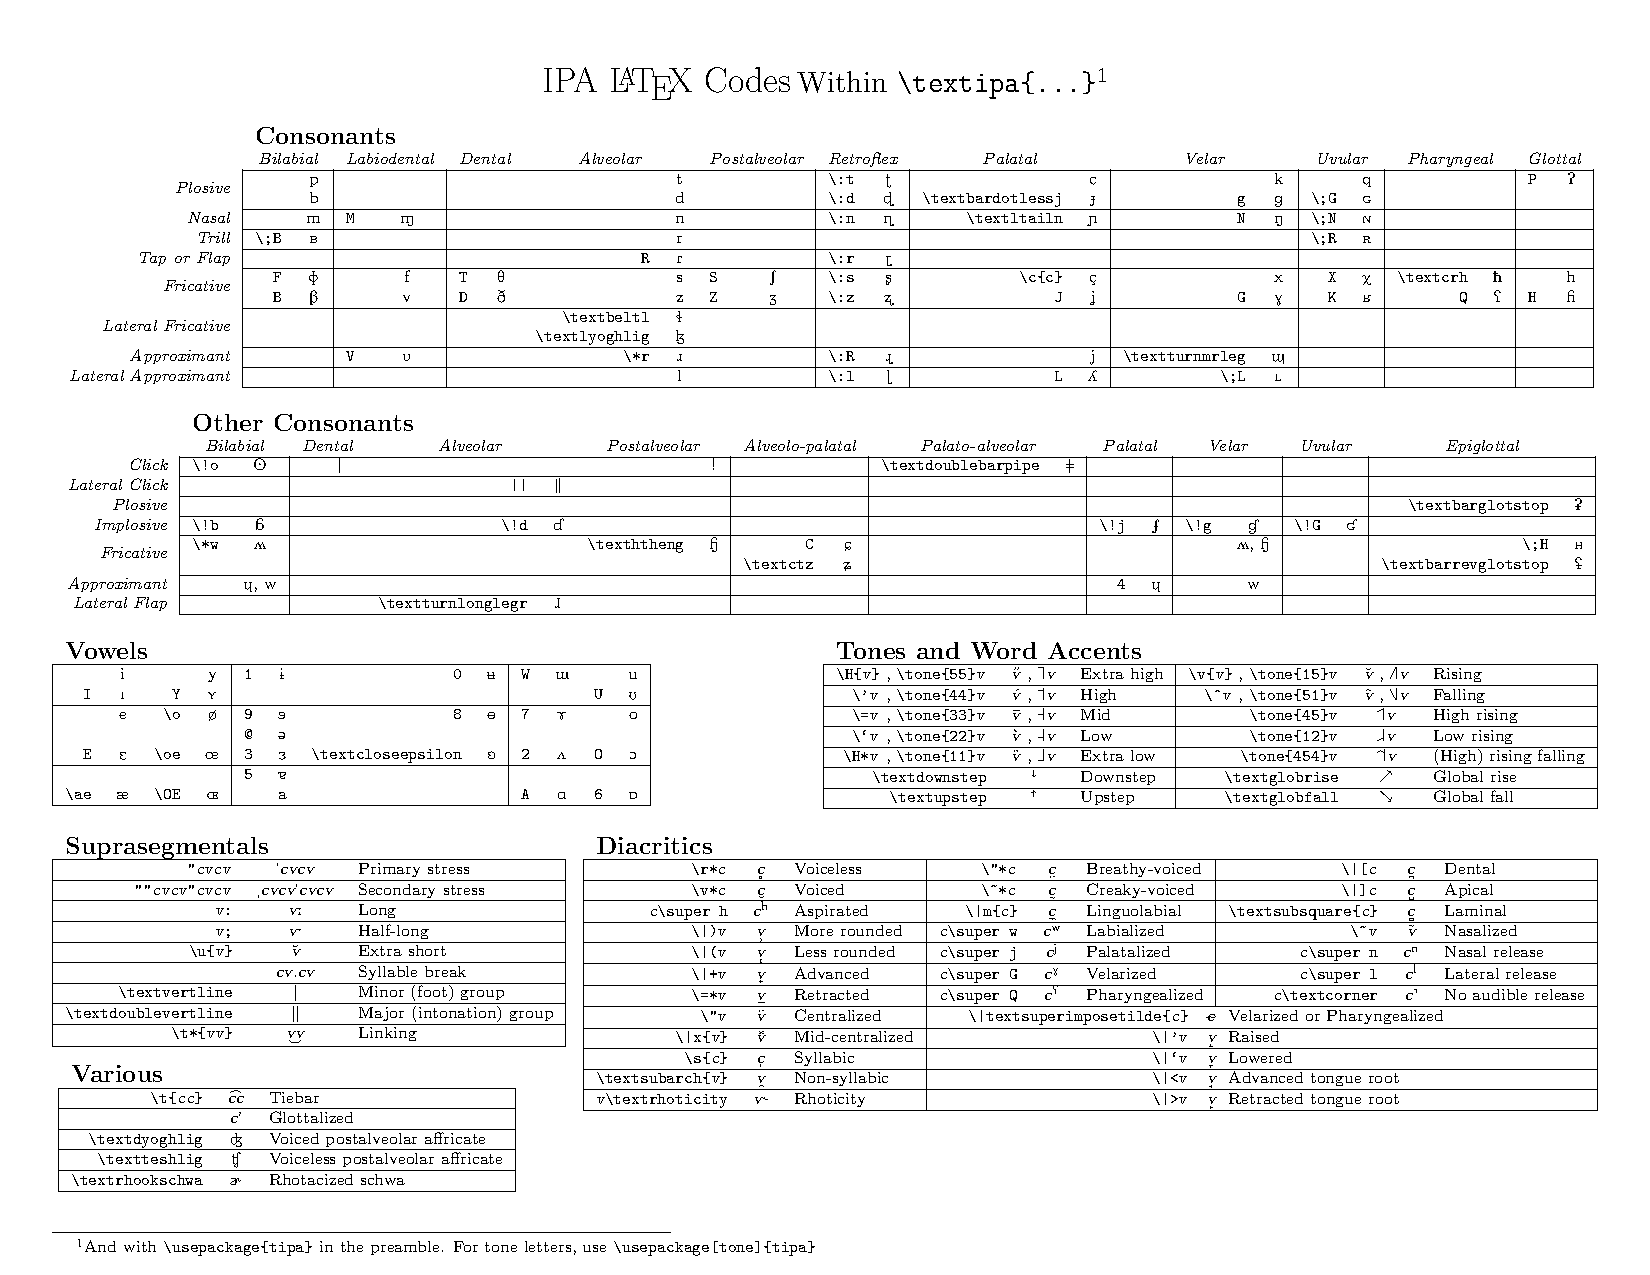
\includegraphics[width=0.7\textwidth,height=0.9\textheight,keepaspectratio]
                     {figures/tipachart_mod.pdf}
  %\caption{Tabela IPA.}
\end{figure}
\end{frame}


\begin{frame}[fragile]
\frametitle{Linguística}
\framesubtitle{Regras fonológicas}
  \scriptsize
  \begin{verbatim}
\usepackage{phonrule}
  
\phonb{\phonfeat{+stop \\ +consonant \\ +alveolar} }{[\textipa{R}]}
{\phonfeat{+vowel \\ +stressed} }{\phonfeat{+vowel \\ +stressed} }
  \end{verbatim}

  \begin{fmpage}{\textwidth}
\phonb{\phonfeat{+stop \\ +consonant \\ +alveolar} }{[\textipa{R}]}{\phonfeat{+vowel \\ +stressed} }{\phonfeat{+vowel \\ +stressed} }
  \end{fmpage}

\end{frame}


\begin{frame}[fragile]
\frametitle{Linguística}
\framesubtitle{Árvores sintáticas}
  \scriptsize
  \begin{columns}[c]
  \column{.5\textwidth}
  \begin{verbatim}
\usepackage{qtree}

\begin{center}
\Tree [.S [.NP LaTeX ] [.VP [.V is ] 
  [.NP fun ] ] ]
\end{center}
  \end{verbatim}
  \column{.5\textwidth}
  \begin{fmpage}{\textwidth}
\begin{center}
\Tree [.S [.NP LaTeX ] [.VP [.V is ] [.NP fun ] ] ]
\end{center}
  \end{fmpage}
  \end{columns}
\end{frame}

\begin{frame}[fragile]
\frametitle{Linguística}
\framesubtitle{Árvore de dependência}

  \begin{fmpage}{\textwidth}
   \begin{dependency}[theme = simple]
   \begin{deptext}[column sep=1em]
      A \& hearing \& is \& scheduled \& on \& the \& issue \& today \& . \\
   \end{deptext}
   \deproot{3}{ROOT}
   \depedge{2}{1}{ATT}
   \depedge[edge start x offset=-6pt]{2}{5}{ATT}
   \depedge{3}{2}{SBJ}
   \depedge{3}{9}{PU}
   \depedge{3}{4}{VC}
   \depedge{4}{8}{TMP}
   \depedge{5}{7}{PC}
   \depedge[arc angle=50]{7}{6}{ATT}
   \end{dependency}
  \end{fmpage}

\end{frame}



%\subsection{Notas e Citações}\label{sec:notascita}
%\input{notas.tex}

%\subsection{Comandos}\label{sec:comandos}
%\subsection{Comandos}

\begin{frame}[fragile,allowframebreaks]
\frametitle{Comandos}
Kunth definiu 325 primitivas para o \TeX{}.

\vspace{3ex}
O outros motores utilizam mais primitivas.
Veja: \hrefcolor{https://www.overleaf.com/learn/latex/TeX_primitives_listed_by_TeX_engine}{\TeX{} primitives listed by \TeX{ engine}}.


\vspace{3ex}
Outros comandos são definidos como combinações de primitivas ou de outros comandos.

\framebreak 

A formatação com \LaTeX{} é facilitada com a utilização de comandos.
Exemplos de comandos: \verb|\textbf{...}|, \verb|\url{...}|, \verb|\item|, etc.

\vspace{3ex}
Novos commandos podem ser definidos:
\begin{lstlisting}[language=tex, label=lst-comand-def, postbreak=\mbox{$\hookrightarrow$\space}, basicstyle=\fontsize{8}{10}\selectfont\ttfamily]
% comando simples (incluir \usepackage{amsfonts})
\newcommand{\R}{$\mathbb{R}$}

% comando com parametro
\newcommand{\bb}[1]{$\mathbb{#1}$} 

% (incluir \usepackage{hyperref})
\newcommand{\email}[1]{\href{mailto:#1}{#1}}
\end{lstlisting}

\framebreak

Comando com parâmetro opcional:
\begin{LTXexample}
\newcommand{\plusbinomial}[3][2]{(#2 + #3)^#1}

\[ \plusbinomial{x}{y} \]

\[ \plusbinomial[4]{y}{y} \]
\end{LTXexample}
\end{frame}





%\subsection{Bibliografia}\label{sec:bibtex}
%\input{bibliografia.tex}








\subsection{Listas}
\begin{frame}
\frametitle{Listas}
\begin{itemize}
\item numeradas
\item não numeradas
\item aninhadas
\end{itemize}
\end{frame}


\begin{frame}[fragile]
\frametitle{Lista não-numerada em \LaTeX{}}
\begin{LTXexample}
\begin{itemize}
\item abacate
\item banana
\item laranja
\end{itemize}
\end{LTXexample}
\end{frame}


\begin{frame}[fragile]
\frametitle{Lista numerada em \LaTeX{}}
\begin{LTXexample}
\begin{enumerate}
\item abacate
\item banana
\item laranja
\end{enumerate}
\end{LTXexample}
\end{frame}


\begin{frame}[fragile]
\frametitle{Lista numerada em \LaTeX{}}
\begin{LTXexample}
\begin{enumerate}[a)]
 \item item a
 \item item b
 \item item c
\end{enumerate}
\end{LTXexample}
\end{frame}


\begin{frame}[fragile]
\frametitle{Lista numerada em \LaTeX{}}
\begin{verbatim}
\begin{enumerate}[label=(\alph*)]
\item abacate
\item banana
\item laranja
\end{enumerate}
\end{verbatim}

obs: incompatível com \texttt{beamer}.
\end{frame}


\begin{frame}[fragile]
\frametitle{Lista aninhada em \LaTeX{}}
\begin{LTXexample}
\begin{enumerate}
\item banana
    \begin{enumerate}
    \item prata
    \item da terra
    \end{enumerate}
\item laranja
    \begin{enumerate}
    \item pera rio
    \item serra d'agua
    \end{enumerate}
\end{enumerate}
\end{LTXexample}
\end{frame}

\begin{frame}[fragile]
\frametitle{Lista de definições em \LaTeX{}}
\begin{LTXexample}
\begin{description}
 \item[primeiro item] txt1 txt1 txt1
 \item[segundo item] txt2 txt2 txt2
 \item[terceiro item] txt3 txt3 txt3
\end{description}
\end{LTXexample}
\end{frame}



\subsection{Citações e notas de rodapé}
\begin{frame}
\frametitle{Citações, notas de rodapé e acrônimos}
Utilize citações e notas de rodapé com parcimônia.

\vspace{3ex}
Evite acrônimos (exceto quando já forem palavras utilizadas na língua franca do assunto abordado).
\end{frame}

\begin{frame}[fragile,allowframebreaks]
\frametitle{Citações}
Em \LaTeX{} utilize os comandos \verb|\cite{...}| e \verb|\textcite{...}| para criar citações.

\vspace{1ex}
Exemplos:
\begin{itemize}
\item \verb|\cite{knuth_texbook_1984}| $\rightarrow$ \cite{knuth_texbook_1984}
\item \verb|\textcite{knuth_texbook_1984}| $\rightarrow$ \textcite{knuth_texbook_1984}
\end{itemize}

\begin{lstlisting}[language=tex, label=lst-bib, caption={Arquivo \texttt{.bib}.}, postbreak=\mbox{$\hookrightarrow$\space}, basicstyle=\fontsize{8}{10}\selectfont\ttfamily]
@book{knuth_texbook_1984,
    title = {The {TeXbook}},
    publisher = {Addison Wesley},
    author = {Knuth, Donald E.},
    year = {1984}
}
\end{lstlisting}

\framebreak

Uma citação textual pode ser feita utilizando o ambiente \verb|quote|.

\begin{LTXexample}
\begin{quote}
Formatting is no substitute for writing. Good ideas couched in
good prose will be read and understood, regardless of how badly the document
is formatted. \LaTeX{} was designed to free you from formatting concerns, allowing
you to concentrate on writing. If you spend a lot of time worrying about form,
you are misusing \LaTeX{}.
\end{quote}
\end{LTXexample}
\cite{lamport_latex_1994}

\framebreak

\begin{itemize}
\item \texttt{bibtex} e \texttt{biber} são programas para processar a bibliografia
\item \texttt{natbib} e \texttt{biblatex} são pacotes de \LaTeX{} para formatar citações e bibliografias
\item \texttt{biblatex-abnt} é um estilo para o padrão ABNT no \texttt{biblatex} 
\end{itemize}

\vspace{2ex}
Sugestões de leitura:
\begin{itemize}
\item[--] \url{https://en.wikibooks.org/wiki/LaTeX/Bibliography_Management}
\item[--] \hrefcolor{https://tex.stackexchange.com/a/25702/37214}{bibtex vs. biber and biblatex vs. natbib (tex.stackexchange.com)}
\end{itemize}
\end{frame}

\begin{frame}[fragile,allowframebreaks]
\frametitle{ABNT - BibLaTeX}
\hrefcolor{https://github.com/abntex/biblatex-abnt}{biblatex-abnt} é um estilo para BibLaTeX compatível com as normas da ABNT.

\vspace{5ex}
\begin{verbatim}
\usepackage[style=abnt]{biblatex}
\addbibresource{arquivo.bib}
\end{verbatim}

\framebreak

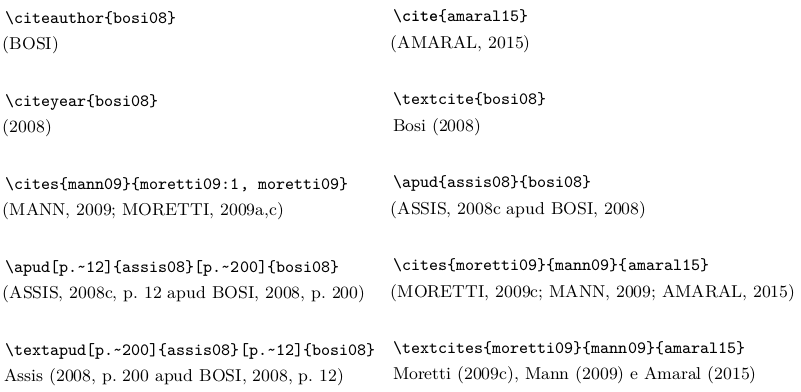
\includegraphics[width=0.8\textwidth,height=0.7\textheight,keepaspectratio]{figures/abnt-example.png}
\end{frame}



\begin{frame}
\frametitle{Dica - Bibliografia}

\begin{itemize}
 \item \hrefcolor{https://zbib.org/}{zoterobib}
 \item \hrefcolor{https://www.doi2bib.org/}{https://www.doi2bib.org/}
 \item \hrefcolor{https://books.google.com}{Google Books}
 \item \hrefcolor{https://www.xarg.org/tools/isbn-to-bibtex/}{https://www.xarg.org/tools/isbn-to-bibtex/}
 \item \hrefcolor{https://www.ottobib.com/}{https://www.ottobib.com/} 
 \item \hrefcolor{https://manas.tungare.name/software/isbn-to-bibtex}{https://manas.tungare.name/software/isbn-to-bibtex}
 \item \hrefcolor{https://arxiv2bibtex.org/}{https://arxiv2bibtex.org/}
\end{itemize}

\vspace{3ex}
Existem ainda vários pacotes para fazer citações, epígrafes, etc.
Veja alguns exemplos no \hrefcolor{https://www.overleaf.com/learn/latex/Typesetting_quotations}{Overleaf}.

\end{frame}



\begin{frame}[fragile,allowframebreaks]
\frametitle{Acrônimos}

Pacote \texttt{acronym} disponível em: \url{https://www.ctan.org/pkg/acronym}.

\begin{verbatim}
\usepackage{acronym}
\end{verbatim}



Opções:
\begin{description}
\item[footnote] nome completo aparece como nota de rodapé
\item[nohyperlinks] não faz o link com glossário 
\item[printonlyused] imprime apenas os que forem utilizados
\item[withpage] imprime a página onde foram utilizados pela primeira vez
\item[smaller] utiliza uma fonte menor
\item[nolist] não faz a lista de acrônimos
\end{description}


\begin{LTXexample}
\begin{acronym}
\acro{CTAN}{The Comprehensive \TeX{} Archive Network}
\acro{RMS}{Root-Mean-Square}
\end{acronym}

\lipsum[1][1-2] \ac{CTAN} \lipsum[1][3] \ac{RMS}.
\lipsum[1][4] \ac{CTAN}, \lipsum[1][5] \ac{RMS}.
\end{LTXexample}

\end{frame}


\begin{frame}[fragile]
\frametitle{Notas de rodapé}
As notas de rodapé têm a finalidade de prestar algum esclarecimento ou informação adicional sobre
algum ponto no texto. Elas são utilizadas para evitar o interrompimento da sequência lógica no texto.

\vspace{2ex}
Notas de rodapé são feitas com o comando \verb|\footnote{...}|. 
Veja aqui\footnote{Exemplificando como criar uma nota de rodapé em \LaTeX{}.} um exemplo de nota de rodapé.
\end{frame}


\subsection{Rótulos e referências}

\begin{frame}[fragile]
\frametitle{Rótulos e referências internas}
Em um texto em \LaTeX{} é possível referenciar quase tudo que é numerado em um documento.
Por exemplo: figuras, tabelas, listas, páginas, secções, capítulos, equações, notas de rodapé, etc.
\pause

\vspace{3ex}
\begin{itemize}[<+->]
\item \verb|\label{rotulo}|: fornecer um rótulo ao objeto que se deseja referenciar
\item \verb|\ref{rotulo}|: realizar a referencia ao objeto com um dado rótulo
\item \verb|\pageref{rotulo}|: referenciar a página onde o objeto se encontra
\end{itemize}

\end{frame}


\begin{frame}[fragile]
\frametitle{Rótulos e referências internas}
\begin{LTXexample}
O teorema de Pit\'agoras \'e equacionado como
\begin{equation}
\label{eq-pitagoras}
c^2 = a^2 + b^2
\end{equation}

...

Veja a Equa\c{c}\~ao~\ref{eq-pitagoras}.
\end{LTXexample}
\end{frame}



\subsection{Equações}
\begin{frame}[fragile]
\frametitle{Equações}
O \LaTeX{} contém as ferramentas necessárias para escrever equações em um documento simples.
Para um documento científico, deve-se utilizar os pacotes \texttt{amsmath} ou \texttt{mathtools}.

\begin{verbatim}
\usepackage{amsmath}
\end{verbatim}

Inserindo fórmulas:
  \begin{itemize}
  \item \emph{inline} (no meio do texto) utilize \verb|\( ... \)| ou \verb|$ ... $|
  \item para equações destacadas do texto utilize \verb|\[...\]| ou \verb|$$...$$| ou o ambiente \texttt{equation} ou \texttt{align}
  \end{itemize}
\end{frame}

\begin{frame}[fragile,allowframebreaks]
\frametitle{Equações}
\framesubtitle{Exemplos}

\begin{LTXexample}
\lipsum[1][1]
$\forall x \in X, \quad \exists y \leq \epsilon$
\lipsum[1][2]
\end{LTXexample}

\begin{LTXexample}
\(\alpha, \beta, \gamma, \delta, \epsilon, \zeta, \eta, \theta, \Gamma, \Delta, \Theta, \Lambda, \pi, \Pi, \phi, \Phi\)
\end{LTXexample}

\begin{LTXexample}
\lipsum[1][1]
\begin{equation}
\cos (2\theta) = \cos^2 \theta - \sin^2 \theta
\end{equation}
\lipsum[1][2]
\end{LTXexample}

\begin{LTXexample}
\lipsum[1][1-2]
\[ \lim_{x \to \infty} \exp(-x) = 0 \]
\lipsum[1][3-4]
\end{LTXexample}

\begin{LTXexample}
$x \equiv a \pmod b$
\end{LTXexample}

\begin{LTXexample}
$k_{n+1} = n^2 + k_n^2 - k_{n-1}$
\end{LTXexample}

\begin{LTXexample}
\begin{equation}
f(n) = \left. n^5 + 4n^2 + 2 \right|_{n=17}
\end{equation}
\end{LTXexample}

\begin{LTXexample}
$(\cdot), [\cdot], \{\cdot\}, |\cdot|, \lVert\cdot\rVert, \langle\cdot\rangle, \lfloor\cdot\rfloor, \lceil\cdot\rceil$
\end{LTXexample}

\begin{LTXexample}
\begin{equation}
\frac{n!}{k!(n-k)!} = \binom{n}{k} = {n \choose k}
\end{equation}
\end{LTXexample}

\begin{LTXexample}
\begin{equation}
\frac{\frac{1}{x}+\frac{1}{y}}{y-z}
\end{equation}
\end{LTXexample}

\begin{LTXexample}
\begin{equation}
x = a_0 + \frac{1}{a_1 + \frac{1}{a_2 + \frac{1}{a_3 + a_4}}}
\end{equation}
\end{LTXexample}

\begin{LTXexample}
\begin{equation}
\frac{
    \begin{array}[b]{r}
      \left( x_1 x_2 \right)\\
      \times \left( x'_1 x'_2 \right)
    \end{array}
  }{
    \left( y_1y_2y_3y_4 \right)
  }
\end{equation}
\end{LTXexample}

\begin{LTXexample}
\begin{equation}
\sqrt[n]{1+x+x^2+x^3+\ldots}
\end{equation}
\end{LTXexample}

\begin{LTXexample}
\lipsum[1][1] $\sum_{i=1}^{10} t_i$ \lipsum[1][2]
\end{LTXexample}

\begin{LTXexample}
\lipsum[1][1] $$ \int_0^\infty e^{-x}\,\mathrm{d}x $$ \lipsum[1][2]
\end{LTXexample}

\begin{LTXexample}
\begin{equation}
 \sum_{\substack{
    0<i<m \\
    0<j<n
 }}
 P(i,j)
\end{equation}
\end{LTXexample}

\begin{LTXexample}
$$\int\limits_a^b$$
\end{LTXexample}

\begin{LTXexample}
$\prod \bigoplus \bigotimes \bigcup \bigcap \oint \iint \iiint$
\end{LTXexample}

\begin{LTXexample}
$$\left(\frac{x^2}{y^3}\right)$$
\end{LTXexample}

\begin{LTXexample}
$$\left.\frac{x^3}{3}\right|_0^1$$
\end{LTXexample}

\begin{LTXexample}
\begin{equation}
\begin{matrix}
  a & b & c \\
  d & e & f \\
  g & h & i
 \end{matrix}
\end{equation}
\end{LTXexample}

\begin{LTXexample}
\begin{equation}
\label{eqn-Amn}
 A_{m,n} =
 \begin{pmatrix}
  a_{1,1} & a_{1,2} & \cdots & a_{1,n} \\
  a_{2,1} & a_{2,2} & \cdots & a_{2,n} \\
  \vdots  & \vdots  & \ddots & \vdots  \\
  a_{m,1} & a_{m,2} & \cdots & a_{m,n}
 \end{pmatrix}
\end{equation}

Conforme a Eq. \ref{eqn-Amn}.
\end{LTXexample}

\begin{LTXexample}
\begin{equation}
f(n) = \left\{ 
\begin{array}{l l}
n/2 & \quad \text{if $n$ is even}\\
-(n+1)/2 & \quad \text{if $n$ is odd}\\
\end{array} \right.
\end{equation}
\end{LTXexample}

\begin{LTXexample}
\begin{eqnarray*}
\cos 2\theta & = & \cos^2 \theta - 
                   \sin^2 \theta \\
             & = & 2 \cos^2 \theta - 1.
\end{eqnarray*}
\end{LTXexample}

\begin{LTXexample}
\begin{align*}
  z_0 &= d = 0 \\
  z_{n+1} &= z_n^2+c
\end{align*}
\end{LTXexample}

\end{frame}


\begin{frame}
\frametitle{Mais informações e exemplos}

\begin{itemize}
\item \href{http://tug.ctan.org/info/short-math-guide/short-math-guide.pdf}{Short Math Guide for \LaTeX}
\item \url{https://www.overleaf.com/learn/latex/Mathematical_expressions}
\item \url{https://en.wikibooks.org/wiki/LaTeX/Mathematics}
\item \url{https://en.wikibooks.org/wiki/LaTeX/Advanced_Mathematics}
\item \url{https://en.wikibooks.org/wiki/LaTeX/Theorems}
\end{itemize}

\end{frame}


\begin{frame}
\frametitle{Dicas para iniciantes}

\begin{itemize}
\item \hrefcolor{https://detexify.kirelabs.org}{Detexify}
\item \hrefcolor{https://www.latex4technics.com/}{LaTeX4technics}
\item \hrefcolor{https://www.mathcha.io/}{Editor de equações online}
\item \hrefcolor{http://www.wolframalpha.com/input/?i=int+sin{x^2}\%2Bsqrt{x}+dx}{Notação TeX e computação no Wolfram Alpha}
\end{itemize}
\end{frame}


\subsection{Comandos}

\begin{frame}[fragile,allowframebreaks]
\frametitle{Comandos}
Kunth definiu 325 primitivas para o \TeX{}.

\vspace{3ex}
O outros motores utilizam mais primitivas.
Veja: \hrefcolor{https://www.overleaf.com/learn/latex/TeX_primitives_listed_by_TeX_engine}{\TeX{} primitives listed by \TeX{ engine}}.


\vspace{3ex}
Outros comandos são definidos como combinações de primitivas ou de outros comandos.

\framebreak 

A formatação com \LaTeX{} é facilitada com a utilização de comandos.
Exemplos de comandos: \verb|\textbf{...}|, \verb|\url{...}|, \verb|\item|, etc.

\vspace{3ex}
Novos commandos podem ser definidos:
\begin{lstlisting}[language=tex, label=lst-comand-def, postbreak=\mbox{$\hookrightarrow$\space}, basicstyle=\fontsize{8}{10}\selectfont\ttfamily]
% comando simples (incluir \usepackage{amsfonts})
\newcommand{\R}{$\mathbb{R}$}

% comando com parametro
\newcommand{\bb}[1]{$\mathbb{#1}$} 

% (incluir \usepackage{hyperref})
\newcommand{\email}[1]{\href{mailto:#1}{#1}}
\end{lstlisting}

\framebreak

Comando com parâmetro opcional:
\begin{LTXexample}
\newcommand{\plusbinomial}[3][2]{(#2 + #3)^#1}

\[ \plusbinomial{x}{y} \]

\[ \plusbinomial[4]{y}{y} \]
\end{LTXexample}
\end{frame}





\subsection{Erros e avisos}
\begin{frame}
\frametitle{Erros e Avisos}
\framesubtitle{}
\centering
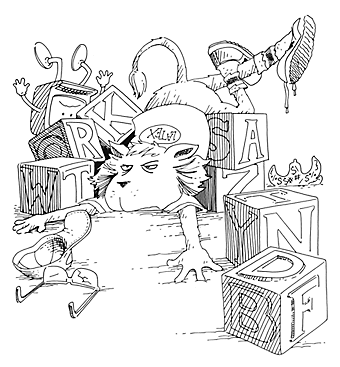
\includegraphics[width=0.4\linewidth,height=0.7\textheight,keepaspectratio]{figures/lion03.png}
\end{frame}

\begin{frame}[fragile]
\frametitle{Erros e Avisos}
\framesubtitle{Errar é inevitável!}

\begin{itemize}
\item achar/reconhecer os seus erros costuma ser a tarefa mais difícil
\item não entre em pânico
\item muitas vezes o erro não está no local onde foi detectado
\end{itemize}

\begin{verbatim}
! Undefined control sequence.

! Too many }'s.

! Missing $ inserted

Runaway argument?

Overfull \hbox 

! LaTeX Error: File `paralisy.sty' not found.
\end{verbatim}
\end{frame}

\begin{frame}[fragile]
\frametitle{Erros e Avisos}
\framesubtitle{Não deixe que os erros virem monstros}
Dica:
\begin{itemize}
\item cada passo de uma vez
\item mantenha um controle de versão (ou backup)
\end{itemize}
\end{frame}

\begin{frame}[fragile]
\frametitle{Coding is like cooking}
\framesubtitle{}
\begin{figure}[h!]
\centering
\label{fig:cooking}
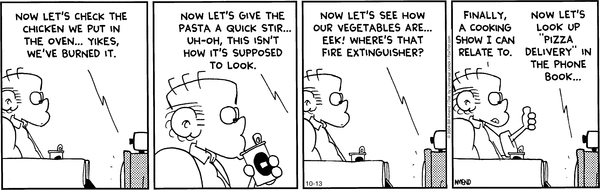
\includegraphics[width=0.8\textwidth,height=0.5\textheight,keepaspectratio]{figures/cooking.png}
\caption{Coding and Cooking (Bill Amend).}
\end{figure}
\end{frame}





\section{LaTeX online}

\begin{frame}[allowframebreaks]
\frametitle{\LaTeX{} online}

\centering
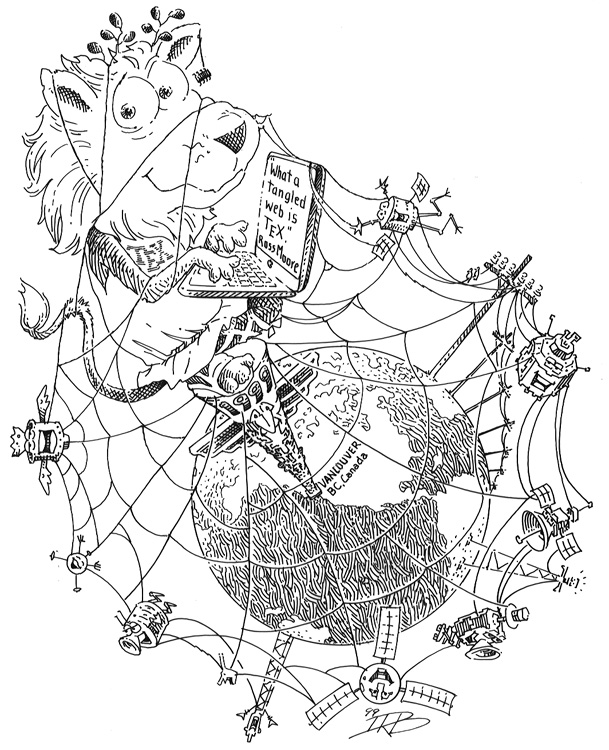
\includegraphics[width=0.4\linewidth,height=0.7\textheight,keepaspectratio]{figures/lion05.png}

\framebreak

\begin{description}
\item[\hrefcolor{https://www.overleaf.com/}{Overleaf}] editor \LaTeX{} colaborativo (em 2017 o Overleaf adquiriu o ShareLaTeX)
\item[\hrefcolor{https://cocalc.com/doc/latex-editor.html}{Cocalc}] é uma plataforma de computação na nuvem com suporte a \LaTeX{}, 
Markdown, HTML, R, Octave, Cython, Julia, Python, ambiente Linux, Jupyter Notebook.
\item[\hrefcolor{https://latexbase.com/}{\LaTeX{} Base}] editor online
\item[\hrefcolor{https://papeeria.com/}{Papeeria}] editor online
\item[\hrefcolor{https://listoffreeware.com/list-of-best-free-online-latex-editors/}{outros}]
\end{description}


Controle de versão
\begin{itemize}
\item Git, Mercurial, Subversion, CVS, etc
\item servidor remoto ou local
\end{itemize}
\end{frame}


\section{Markdown}

\begin{frame}[fragile,allowframebreaks]
\frametitle{Markdown}
*Markdown* é uma linguagem simples de marcação.

\vspace{3ex}
Pode ser utilizada para gerar documentos HTML, RTF, TeX, etc.

\vspace{3ex}
É utilizada (com algumas Variações) em sites como GitHub, Reddit, Diaspora, Stack Exchange, etc.

\vspace{3ex}
A Wikipedia também utiliza uma linguagem simples de marcação, chamada de \emph{wikitext} ou \emph{marcação wiki} ou \emph{wikicode}.

\framebreak 

\lstinputlisting[label=lst-ex-markdown, firstline=1, lastline=16, postbreak=\mbox{$\hookrightarrow$\space}, basicstyle=\fontsize{8}{10}\selectfont\ttfamily]{examples/markdown-ex1.txt}

\framebreak

\lstinputlisting[label=lst-ex-markdown, firstline=18, lastline=32, postbreak=\mbox{$\hookrightarrow$\space}, basicstyle=\fontsize{8}{10}\selectfont\ttfamily]{examples/markdown-ex1.txt}

\framebreak

\lstinputlisting[label=lst-ex-markdown, firstline=34, lastline=46, postbreak=\mbox{$\hookrightarrow$\space}, basicstyle=\fontsize{8}{10}\selectfont\ttfamily]{examples/markdown-ex1.txt}

\framebreak

\begin{itemize}
\item \hrefcolor{https://pandoc.org/}{pandoc} - conversor de documentos
\item \hrefcolor{https://www.ctan.org/pkg/markdown}{pacote de markdown para \LaTeX{}}
\end{itemize}

\end{frame}




\section{Arquivos}
\begin{frame}
\frametitle{Arquivos}
\framesubtitle{}
\centering
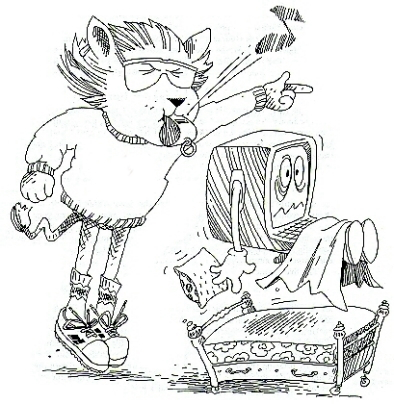
\includegraphics[width=0.4\linewidth,height=0.6\textheight,keepaspectratio]{figures/TexLionWhistle.jpg}
\end{frame}


\begin{frame}
\frametitle{Arquivos}

Arquivos são recursos computacionais para armazenar informações.

\pause 
\vspace{3ex}
O sistema de arquivos organiza e disponibiliza o acesso aos arquivos.

\pause
\vspace{3ex}
Nos sistemas modernos os arquivos são organizados em arranjos lineares de bytes.

\pause
\vspace{3ex}
O formato de um arquivo é definido pelo seu conteúdo. Muitos arquivos possuem um cabeçalho com metadados sobre si mesmo.
\end{frame}

\begin{frame}
\frametitle{Operações sobre arquivos}
\begin{itemize}%[<+->]
\item criar
\item alterar permissões de acesso e atributos
\item abrir
\item ler
\item escrever
\item fechar
\item apagar
\item trucar
\item acrescentar 
\end{itemize}
\end{frame}


\begin{frame}
\frametitle{Organização hierárquica}
\begin{minipage}{0.47\textwidth}
\dirtree{%
.1 spam.
.2 ham.
.2 eggs.
.3 more spam.
.3 dead parrots.
}
\end{minipage}
\hfill
\begin{minipage}{0.47\textwidth}
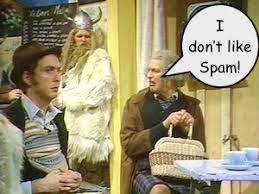
\includegraphics[width=\linewidth,height=0.5\textheight,keepaspectratio]{figures/mp-spam.jpg}
\end{minipage}
\end{frame}

\begin{frame}
\frametitle{Arquivo corrompido}
Dizemos que um arquivo é corrompido quando ele sofre alguma alteração de forma não possa mais ser lido (por software ou por humano). 
\end{frame}

\begin{frame}[fragile,allowframebreaks]
\frametitle{Codificação de arquivos}
\framesubtitle{Representação binária}
Arquivos são armazenados na forma binária no computador. 

\vspace{3ex}
Como exemplo, vamos analisar o arquivo \texttt{introducao.tex}.

\begin{footnotesize}
\begin{verbatim}
$ file introducao.tex 
introducao.tex: LaTeX document, UTF-8 Unicode text, with very long lines

$ ls -l introducao.tex
-rw-r--r-- 1 leoca leoca 9292 nov  1 14:10 introducao.tex
\end{verbatim}
\end{footnotesize}

\framebreak
\begin{footnotesize}
\begin{verbatim}
$ cat introducao.tex | xxd -b | head
00000000: 01011100 01100010 01100101 01100111 01101001 01101110  \begin
00000006: 01111011 01100110 01110010 01100001 01101101 01100101  {frame
0000000c: 01111101 00001010 01011100 01100110 01110010 01100001  }.\fra
00000012: 01101101 01100101 01110100 01101001 01110100 01101100  metitl
00000018: 01100101 01111011 01001111 00100000 01110001 01110101  e{O qu
0000001e: 01100101 00100000 11000011 10101001 00100000 01011100  e .. \
00000024: 01001100 01100001 01010100 01100101 01011000 01111011  LaTeX{
0000002a: 01111101 00111111 01111101 00001010 01011100 01100110  }?}.\f
00000030: 01110010 01100001 01101101 01100101 01110011 01110101  ramesu
00000036: 01100010 01110100 01101001 01110100 01101100 01100101  btitle
\end{verbatim}
\end{footnotesize}

\begin{footnotesize}
\begin{verbatim}
$ echo -n "TeX" | xxd
00000000: 5465 58                                  TeX

$ echo -n "TeX" | xxd -b
00000000: 01010100 01100101 01011000                             TeX
              T        e       X
hex          54       65      58 
dec          84      101      88
oct         124      144     130
\end{verbatim}
\end{footnotesize}
\end{frame}

\begin{frame}
\frametitle{Codificação de arquivos}
\framesubtitle{História}
  The Evolution of Character Codes, 1874-1968\\
  by Eric Fischer

  \vspace{2em}
  \url{https://github.com/ericfischer/ascii}
\end{frame}

\begin{frame}
\frametitle{Codificação de arquivos}
\framesubtitle{Código Morse - Samuel Morse e Alfred Vail (1837)}
        \centering
        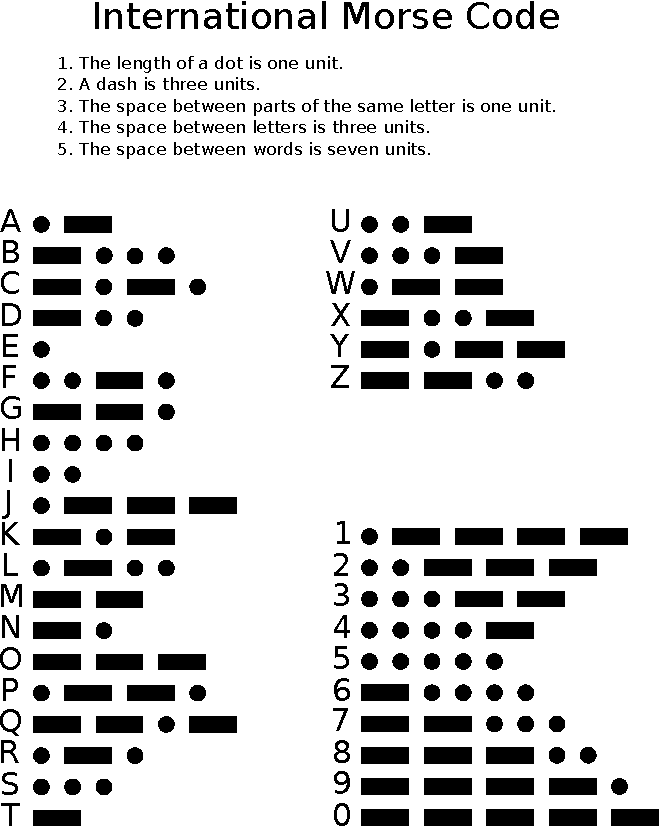
\includegraphics[width=0.3\textwidth,height=0.7\textheight,keepaspectratio]{figures/MorseCode.pdf} \hspace{3em}
        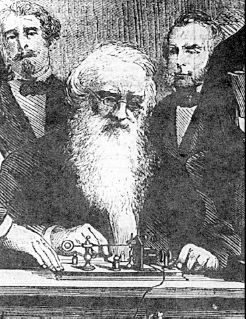
\includegraphics[width=0.3\textwidth,height=0.5\textheight,keepaspectratio]{figures/samuelmorse.jpg}
\end{frame}
\note{
Samuel Morse utilizou códigos de tamanho variável quando projetava o seu conhecido código telegráfico.
Samuel Morse havia sido comissionado em 1825 para pintar um retrato de Lafayette, em uma visita a Washington, DC.
Enquanto pintava, ele recebeu uma mensagem avisando que sua esposa estava muito doente.
Morse partiu imediatamente para sua casa em New Haven. Quando chegou sua esposa já havia sido enterrada.
Ele decidiu então se dedicar a explorar formas de comunicações a longa distância que fossem mais rápidas.

A primeira versão do código, desenvolvida por Morse durante uma viagem transatlântica em 1832,
era mais complexa do que a versão estabelecida em 1843. Mais tarde, Morse abandonou sua versão
em favor dos conhecidos pontos e traços desenvolvidos em conjunto com Alfred Vail.
Morse recebeu a patente do seu telégrafo com um único fio em 1847, sobrepujando o telégrafo
de múltiplos fios proposto por Cooke e Wheatstone, que havia sido patenteado em 1837.
}

\begin{frame}
\frametitle{Codificação de arquivos}
\framesubtitle{Código Baudot e Código Murray}
        \centering
        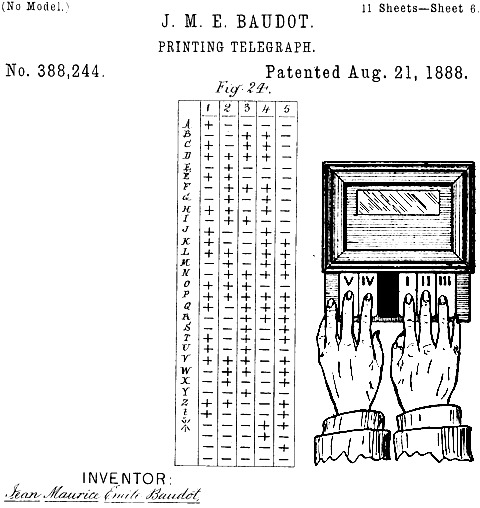
\includegraphics[width=0.3\textwidth,height=0.8\textheight,keepaspectratio]{figures/BaudotCode.png} \hspace{2em}
        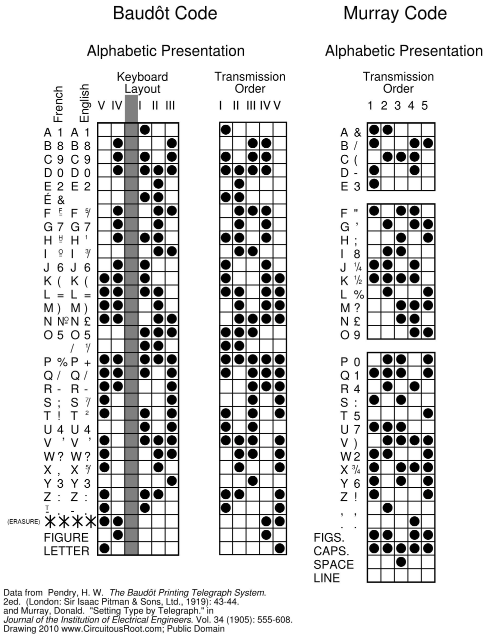
\includegraphics[width=0.35\textwidth,height=0.8\textheight,keepaspectratio]{figures/murraybaudot.png}
\end{frame}
\note{
Na França, Emile Baudout projetou seus sistema para o telégrafo em 1874.
Seu código foi baseado em código anterior desenvolvidos por 
Carl Friedrich Gauss e Wilhelm Weber em 1834.
Todos os símbolos possuem o mesmo comprimento, cinco. O projeto utilizava
um conjunto de fios funcionando de forma síncrona em um sistema de multiplexação,
onde o operador humano era responsável por realizar a divisão temporal e assim a sincronização.
Os códigos eram gerados por um aparelho com cinco teclas (similar às teclas de um piano),
sendo operado com duas mãos (dois dedos da mãos esquerda e três da mão direita).

Quando ordenados em alfabeticamente, as vogais e as consoantes, formam um código de Gray.

O código Baudout foi projetado para minimizar os movimentos da mão e dedos,
reduzindo assim a fadiga.
}\note{
O código de Baudout foi modificado por Donald Murray (1901) para ser utilizado
em um aparelho com teclado QWERTY. A mensagem é gravada em uma fita através de perfurações
e transmitida a partir desta fita perfurada. Deixou assim de existir a conexão direta entre
a mão do operador e a informação transmitida, não sendo mais necessário preocupar-se com a fadiga.
O objetivo passou então a ser simplificar o equipamento e minimizar seu desgaste, para tanto as
combinações com menos buracos foram utilizadas para designar caracteres mais frequentes
(ordem de freq. de occ. no inglês: e,t,a,o,i,n,s,h,r,d,l,c,u,m,w,f,g,y,p,b,v,k,j,x,q,z).


O código Murray também introduziu os caracteres de controle CR (carriage return) e
LF (line feed).
}


\begin{frame}
\frametitle{Codificação de arquivos}
\framesubtitle{Código Murray}
        \centering
        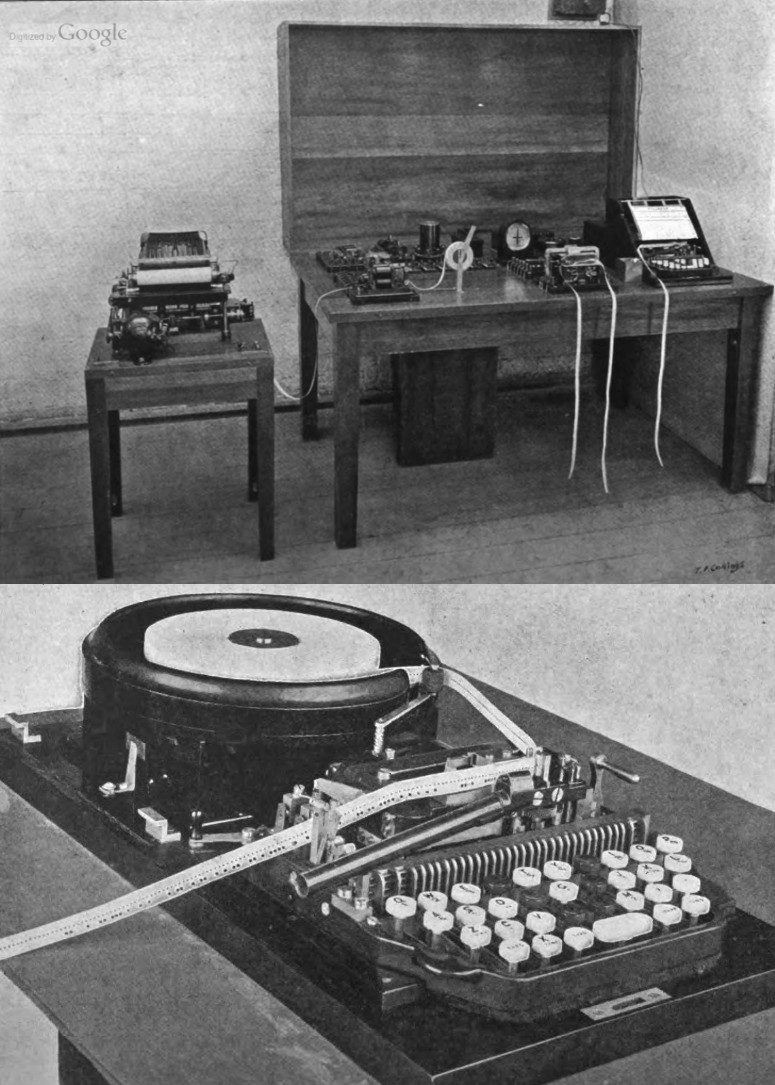
\includegraphics[width=0.35\textwidth,height=0.8\textheight,keepaspectratio]{figures/murrayapparatus.jpg} 
\end{frame}


\begin{frame}
\frametitle{Codificação de arquivos}
\framesubtitle{Western Union e ITA2}
   \begin{itemize}
   \item O código Murray foi adotado pelo Western Union com algumas modificações, sendo utilizado até os anos 50.
   \item Em 1924 o CCITT\footnote{O CCITT (International Telegraph and Telephone Consultative Committee) hoje conhecido
                                 como ITU-T (ITU Telecommunication Standardization Sector), um dos três setores do
                                 ITU (International Telecommunication Union) responsável pela definição de padrões em telecomunicações.}
         criou o ITA2 (international telegraph alphabet n. 2), baseado no código da Western Union.
   \item ITA2, também chamado de US TTY (American Teletypewriter code) foi a base para codificação em 5 bits dos Teletipos
         até o surgimento do código de 7 bits, ASCII em 1963.
   \end{itemize}
\end{frame}


\begin{frame}
\frametitle{Codificação de arquivos}
\framesubtitle{ASCII 1963 (7 bits)}
\centering
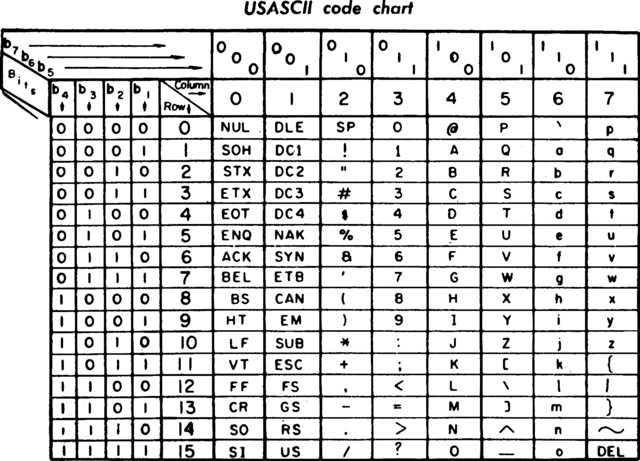
\includegraphics[width=0.65\textwidth,height=0.8\textheight,keepaspectratio]{figures/USASCII.png}
\end{frame}
\note{
\scriptsize
Foi desenvolvido pelo Comitê X3 da ASA (American Standards Association),
da qual faziam parte IBM (embora só passou a adotar o ASCII na década de 80),
AT\&T e sua subsidiária Teletype Corporation.

Os caracteres estão organizados de forma que os caracteres alfabéticos,
numéricos, matemáticos e de controle podem ser isolados através de uma
simples máscara binária.

O caractere A fica na posição $41_{\textmd{hex}}$ para ser compatível com o padrão
britânico. Os dígitos de 0 a 9 começam com $011$ e a sequência binária seguinte
corresponde ao valor binários de cada um deles, facilitando assim a conversão decimal-binário.

Os caracteres !"\#\$\%\&() foram adicionados à 2 coluna de forma a melhor se adequarem
à posição que ocupavam nos teclados das máquinas de escrever, de forma que a tecla \textit{shift}
corresponderia à uma simples mudança de um bit, assim facilitando a compatibilidade com as máquinas de escrever.

Foi cogitado utilizar um código com 8 bits, de forma que dois padrões de 4 bits
codificariam 2 dígitos. Isto iria requerer que fosse enviado sempre 8 bits.
Para minimizar custos, adotou-se 7 bits. Como as fitas perfuradas podiam armazenar
8 bits em cada posição, seria ainda possível utilizar um bit de paridade se desejado.
}


\begin{frame}
\frametitle{Codificação de arquivos}
\framesubtitle{Códigos de 8 bits}
  \begin{itemize}
  \item Extended ASCII 
  \item ISO/IEC 8859
  \item Windows-1252 (CP-1252)
  \end{itemize}

  Existem mais de 220 extensões DOS/Windows e 
  mais de 186 extensões EBCDIC (Extended Binary Coded Decimal Interchange Code),
  majoritariamente usado pela IBM.

  Dentre os padrões ISO o mais popular é o ISO 8859-1, também conhecido como ISO Latin 1,
  contendo a maioria dos caracteres utilizados pelas línguas da Europa Ocidental.
\end{frame}
\note{
A popularização do IBM System/360 e microprocessadores como o
Intel 8008, 8080 e 8086 acarretou na padronização do byte como uma unidade de 8 bits.
Endereçamento e armazenamento passaram a ser feitos em 8 bits, assim possibilitou a
extensão do ASCII utilizando o bit extra.
}

\begin{frame}
\frametitle{Codificação de arquivos}
\framesubtitle{Códigos Multi-Byte}
  \begin{itemize}
  \item Podem representar mais do que 256 caracteres.
  \item Alguns são extensões do ASCII (compatibilidade). Exemplo: UTF-8.
  \item UTF-16 não é uma extensão do ASCII pois os caracteres ASCII são armazenados em dois bytes, um deles igual a 0x00.
  \end{itemize}
\end{frame}

\begin{frame}[allowframebreaks]
\frametitle{Codificação de arquivos}
\framesubtitle{UFT-8}
  \begin{itemize}
  \item UTF-8: Unicode (ou Universal Coded Character Set) Transformation Format - 8-bit.
  \item Utiliza de 1 a 4 bytes.
  \item Capaz de representar até 1.112.064 pontos de codificação do Unicode.
  \item Compatibilidade reversa com ASCII (utiliza um único octeto com mesmo valor binário que o ASCII).
  \item Pontos de código mais usuais utilizam menos bytes que aqueles menos comuns.
  \item 128 caracteres ASCII necessitam de um byte (começando com 0). 
  \item 1920 caracteres utilizam 2 bytes para representar o restante do alfabeto latino (romano),
        grego, cirílico, copta, armênio, hebreu, arábico, siríaco, thaana e n'ko.
  \item Para as demais línguas são utilizados 3 bytes.
  \item 4 bytes para caracteres como símbolos matemáticos e emojis.
  \item O primeiro byte determina o número de bytes na sequência.
  \item UTF-8 foi apresentado em uma conferência em 1993. Em 2003 foi registrado pela RFC 3629 e 
        em 2008 tornou-se o padrão mais utilizado na internet.
  \item Criado por Ken Thompson e Rob Pike.
  \end{itemize}


  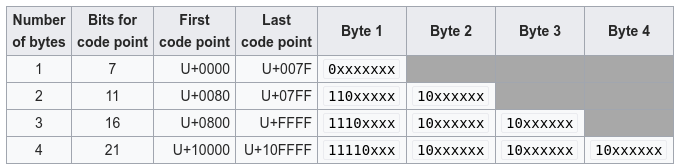
\includegraphics[width=0.85\textwidth,height=0.35\textheight,keepaspectratio]{figures/utf8bytes.png}

  {
  \centering
  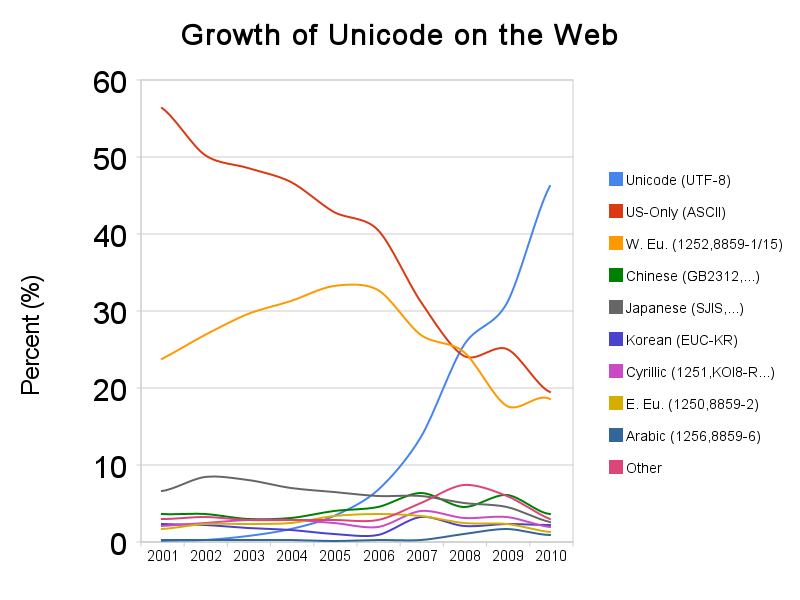
\includegraphics[width=0.55\textwidth,height=0.8\textheight,keepaspectratio]{figures/unicodeweb.png} 
  }
  \footnotesize{googleblog: \url{https://googleblog.blogspot.com.br/2010/01/unicode-nearing-50-of-web.html}}
  

  {
  \centering
  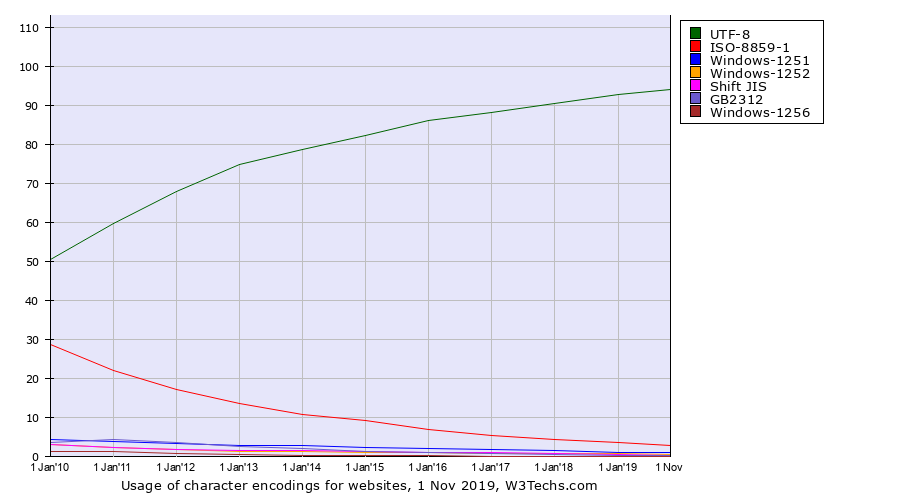
\includegraphics[width=0.6\textwidth,height=0.8\textheight,keepaspectratio]{figures/w3usage.png}
  }
  \footnotesize{W3Techs: \url{https://w3techs.com/technologies/history_overview/character_encoding/ms/y}}
\end{frame}

\begin{frame}
\frametitle{Codificação de arquivos}
\framesubtitle{Unicode}
  O Unicode é uma padrão para a industria de computadores para estabelecer uma 
  codificação, representação e manipulação consistente de textos utilizados por grande parte dos
  sistemas de escrita do mundo.

  A última versão do Unicode possui 136.755 caracteres cobrindo 139 escritas modernas e antigas, 
  e também outros conjuntos símbolos utilizados na comunicação humana (por exemplo, símbolos matemáticos
  e emojis).

  O Unicode é mantido pelo Consórcio do Unicode, criado em 1991, cujos membros incluem Adobe, Apple, Google, Huawei, IBM,
  Microsoft, Oracle, Yahoo! e SAP.
\end{frame}

\begin{frame}[allowframebreaks]
\frametitle{Codificação de arquivos}
\framesubtitle{Extremidade (\textit{endianness})}
  O termo \textbf{extremidade} (endianness) refere-se a ordem utilizada para armazenar/ler os bytes ou bits de dados.

  Byte 
  \hrule
  \begin{description}
  \item[big-endian]: extremidade maior primeiro -  Motorola (famílias 6800 e 68000), PowerPC (Apple).
  \item[little-endian]: extremidade menor primeiro - Intel (x86), AMD, Zilog (Z80), MOS Technology (6502), DEC (VAX e PDP-11).
  \end{description}

  Bit
  \hrule
  \begin{description}
  \item[LSB 0]: a numberação dos bits inicia-se pelo menos significante - SPARC e Motorola 68000.
  \item[MSB 0]: a numberação dos bits inicia-se pelo mais significante - S/390, PowerPC e PA-RISC (recomendada pela RfC).
  \end{description}

  \framebreak
  \begin{itemize}
  \item Lilliput - Viagens de Gulliver (Jonathan Swift).
  \item Unicode - marcador BOM (Byte Order Mark) - ponto de representação \texttt{U+FEFF}.
  \item No UTF-8 o marcador BOM é representado pela sequência de 3 octetos: \texttt{0xEF,0xBB,0xBF} (1110 1111 1011 1011 1011 1111).
  \item Extremidade (byte) é irrelevante para o padrão UTF-8 e portanto o marcador BOM é desnecessário.
  \item No padrão UTF-16 a sequência de bytes \texttt{0xFE,0xFF} indica ordenação \textit{big-endian} e a sequência \texttt{0xFF,0xFE}
        indica a ordenação \textit{little-endian}.
  \end{itemize}

  \hfill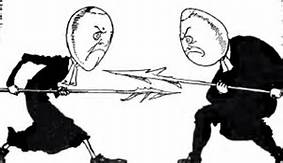
\includegraphics[width=0.2\textwidth,height=0.3\textheight,keepaspectratio]{figures/lilliputwar.jpg}
\end{frame}
\note{
As CPUs que utilizam \textit{little-endian} usualmente usam o `LSB 0', enquanto
as CPUs que utilizam \textit{big-endian} utilizam ambas padronizações.
O estilo recomendado pela RfC (Request for Comments) é `MSB 0'.
Algumas arquiteturas, como SPARC e Motorola 68000 utilizam `LSB 0', enquanto
S/390, PowerPC e PA-RISC utilizam `MSB 0'.
}
\note{
``O termo em inglês para uma forma de \emph{endianness}, \emph{big-endian}, é uma referência às Viagens de Gulliver: 
em Lilliput houve uma guerra civil, entre os que preferiam quebrar os ovos cozidos pelo lado maior (big-endians) 
contra quem preferia quebrar os ovos cozidos pelo lado menor. Este conflito, por sua vez, era uma paródia 
entre as diferenças entre católicos e protestantes a respeito da transubstanciação.'' (Wikipedia)
\url{https://pt.wikipedia.org/wiki/Extremidade\_(ordena\\\%C3\\\%A7\\\%C3\\\%A3o)}
}

\begin{frame}[fragile]
\frametitle{Determinando a codificação}

O comando \texttt{file} do Linux/Unix/OS X/macOS tenta `adivinhar' qual é a codificação do arquivo.

\begin{lstlisting}[language=bash, label=lst-filecod, caption={Determinando o tipo de codificação de um arquivo.}, postbreak=\mbox{$\hookrightarrow$\space}, basicstyle=\fontsize{8}{10}\selectfont\ttfamily]
$ file -i arquivo.csv
arquivo.csv: application/csv; charset=us-ascii
$ file -i arquivo.xls 
arquivo.xls: text/plain; charset=utf-16le
$ file -i imagem.png 
imagem.png: image/png; charset=binary
$ file -i imagem.jpg 
imagem.jpg: image/jpeg; charset=binary
\end{lstlisting}
\end{frame}

\begin{frame}[fragile]
\frametitle{Convertendo o tipo de codificação}
O comando \texttt{iconv} converte um tipo de codificação de caracteres em outro tipo. Faz a conversão entre 1179 tipos de codificação.
\begin{lstlisting}[language=bash, label=lst-iconv, caption={Convertendo o tipo de codificação de um arquivo.}, postbreak=\mbox{$\hookrightarrow$\space}, basicstyle=\fontsize{8}{10}\selectfont\ttfamily]
$ iconv -f ISO-8859-1 -t ASCII arquivo.txt > arquivo_ascii.txt
$ iconv -f ISO-8859-1 -t ASCII//TRANSLIT input.file -o out.file
$ iconv -f ISO-8859-1 -t UTF-8//IGNORE input.file -o out.file
\end{lstlisting}
\end{frame}

\begin{frame}[fragile]
\frametitle{Exemplo - declaração de codificação em um HTML}
\begin{lstlisting}[language=html, label=lst-htmlenc, caption={Documento HTML.}, postbreak=\mbox{$\hookrightarrow$\space}, basicstyle=\fontsize{8}{10}\selectfont\ttfamily]
<!DOCTYPE html>
<html lang="en">
<head>
<meta http-equiv="Content-Type" content="text/html; charset=utf-8"/>
\end{lstlisting}
\end{frame}


\begin{frame}[fragile]
\frametitle{A traição dos nomes}
\begin{figure}[h]
\centering
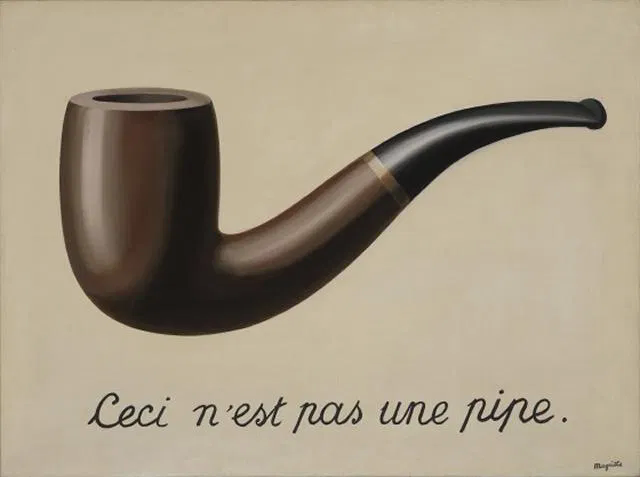
\includegraphics[width=0.5\textwidth,height=0.7\textheight,keepaspectratio]{figures/magritte.png}
\caption{\emph{La trahison des images}, René Magritte (1929).}
\label{fig-magritte}
\end{figure}
\end{frame}
\note{
``Este quadro, uma das obras-primas surrealistas do artista, está atualmente no Museu de Arte do Condado de Los Angeles (LACMA), Califórnia (...)
Fortemente influenciado pela psicologia freudiana, o surrealismo representou uma reação contra o "racionalismo". A Traição das Imagens desafia a convenção linguística de identificar uma imagem de algo como a coisa em si. (...) René Magritte nega aquilo que estamos a ver. A uma primeira análise, o significado desta negação torna-se claro, pois aquilo que estamos a ver não é um cachimbo verdadeiro, mas sim a representação de um cachimbo. Deparamo-nos com um desafio àquilo que se convencionou chamar de "cachimbo", pois a nossa imagem de cachimbo está negada. Magritte como que esvaziou de sentido aquilo que entendemos como sendo a palavra "cachimbo". Não podemos identificar esta representação com aquilo que é o objeto, gerando-se, assim, um conflito de mensagens.''(\hrefcolor{https://pt.wikipedia.org/wiki/A_Trai\%C3\%A7\%C3\%A3o_das_Imagens}{Wikipedia - A Traição das Imagens})
}


\begin{frame}[allowframebreaks]
\frametitle{Formatos de arquivos}
\begin{description}
\item[ASCII, UTF-8](\texttt{.txt}) texto puro 
\item[MS Word](\texttt{.doc} e \texttt{.docx}) formato binário e XML estruturado, respectivamente
\item[DjVu](\texttt{.djvu}) formato utilizado principalmente para documentos escaneados
\item[HTML](\texttt{.html} ou \texttt{.htm}) páginas Web (padrão ISO)
\item[PDF](\texttt{.pdf}) padrão aberto\footnote{O padrão PDF passou a ser um padrão aberto em 1 de julho de 2008.} para troca de documentos (ISO 32000)
\item[PostScript](\texttt{.ps}) linguagem de descrição de página
\item[SVG](\texttt{.svg}) gráficos vetoriais escalonáveis
\item[TeX](\texttt{.tex}) arquivos texto para produção de documentos utilizando \TeX{}
\item[BMP](\texttt{.bmp}) imagens Bitmap do Windows
\item[GIF](\texttt{.gif}) imagens rasterizadas 
\item[PNG](\texttt{.png}) imagens rasterizadas (formato aberto)
\item[JPEG](\texttt{.jpg} ou \texttt{.jpeg}) formato para imagens rasterizadas (compressão com perdas)
\item[WAV](\texttt{.wav}) Microsoft Wave (sem compressão)
\item[FLAC](\texttt{.flac}) formato de áudio com compressão sem perdas
\item[MP3](\texttt{.mp3}) formato de áudio com compressão com perdas (patenteado)
\item[OGG](\texttt{.ogg}) formato aberto de áudio com compressão com perdas 
\end{description}
\end{frame}

\begin{frame}[fragile,allowframebreaks]
\frametitle{Exemplo \texttt{.docx}}

\begin{figure}[h]
\centering
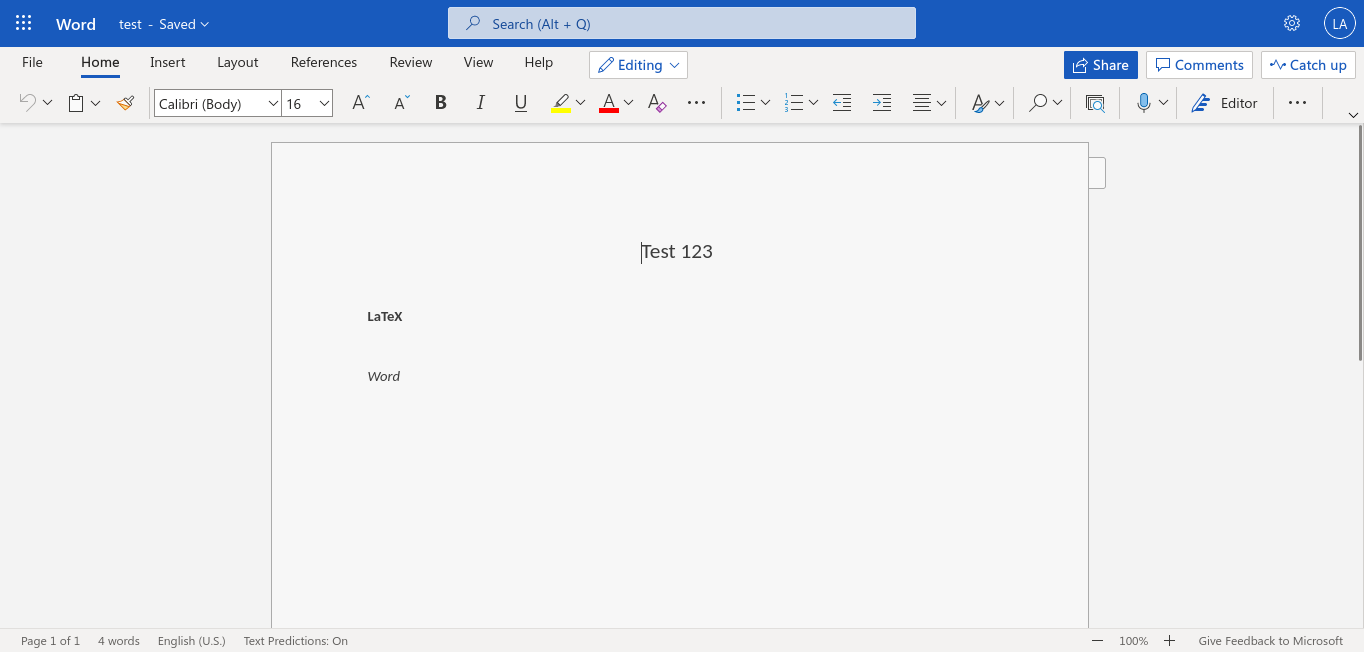
\includegraphics[width=0.8\textwidth,height=0.8\textheight,keepaspectratio]{figures/test-word.png}
\caption{Documento exemplo criado no Office 365.}
\label{fig-word-test}
\end{figure}

\framebreak

\begin{lstlisting}[language=bash, label=lst-docx, caption={Conteúdo do arquivo \texttt{.docx} exemplo. Visualização com \texttt{vim}.}, postbreak=\mbox{$\hookrightarrow$\space}, basicstyle=\fontsize{6}{8}\selectfont\ttfamily]
" zip.vim version v28
" Browsing zipfile /tmp/test.docx
" Select a file with cursor and press ENTER

[Content_Types].xml
_rels/.rels
word/theme/theme1.xml
word/settings.xml
word/fontTable.xml
word/webSettings.xml
docProps/app.xml
docProps/core.xml
word/styles.xml
word/document2.xml
word/_rels/document2.xml.rels
\end{lstlisting}

\framebreak

\begin{lstlisting}[language=xml, label=lst-docx-1, caption={Conteúdo do arquivo \texttt{word/document2.xml}}, postbreak=\mbox{$\hookrightarrow$\space}, basicstyle=\fontsize{6}{8}\selectfont\ttfamily]
<?xml version="1.0" encoding="utf-8" standalone="yes"?><w:document xmlns:wpc="http://schemas.microsoft.com/office/word/2010/wordprocessingCanvas" xmlns:mc="http://schemas.openxmlformats.org/markup-compatibility/2006" xmlns:o="urn:schemas-microsoft-com:office:office" xmlns:r="http://schemas.openxmlformats.org/officeDocument/2006/relationships" xmlns:m="http://schemas.openxmlformats.org/officeDocument/2006/math" xmlns:v="urn:schemas-microsoft-com:vml" xmlns:wp14="http://schemas.microsoft.com/office/word/2010/wordprocessingDrawing" xmlns:wp="http://schemas.openxmlformats.org/drawingml/2006/wordprocessingDrawing" xmlns:w10="urn:schemas-microsoft-com:office:word" xmlns:w="http://schemas.openxmlformats.org/wordprocessingml/2006/main" xmlns:w14="http://schemas.microsoft.com/office/word/2010/wordml" xmlns:w15="http://schemas.microsoft.com/office/word/2012/wordml" xmlns:wpg="http://schemas.microsoft.com/office/word/2010/wordprocessingGroup" xmlns:wpi="http://schemas.microsoft.com/office/word/2010/wordprocessingInk" xmlns:wne="http://schemas.microsoft.com/office/word/2006/wordml" xmlns:wps="http://schemas.microsoft.com/office/word/2010/wordprocessingShape" mc:Ignorable="w14 w15 wp14"><w:body><w:p w:rsidP="4FDD56AD" w14:paraId="2C078E63" xmlns:wp14="http://schemas.microsoft.com/office/word/2010/wordml" wp14:textId="19C3A7FB"><w:pPr><w:jc w:val="center" /><w:rPr><w:b w:val="0" /><w:bCs w:val="0" /><w:sz w:val="32" /><w:szCs w:val="32" /></w:rPr></w:pPr><w:bookmarkStart w:name="_GoBack" w:id="0" /><w:bookmarkEnd w:id="0" /><w:r w:rsidRPr="4FDD56AD" w:rsidR="79861D53"><w:rPr><w:b w:val="0" /><w:bCs w:val="0" /><w:sz w:val="32" /><w:szCs w:val="32" /></w:rPr><w:t>Test 123</w:t></w:r></w:p><w:p w:rsidR="4FDD56AD" w:rsidP="4FDD56AD" w:rsidRDefault="4FDD56AD" w14:paraId="2700AB13" w14:textId="40AAB38F"><w:pPr><w:pStyle w:val="Normal" /></w:pPr></w:p><w:p w:rsidR="79861D53" w:rsidP="4FDD56AD" w:rsidRDefault="79861D53" w14:paraId="53B87EDE" w14:textId="05C1A8EF"><w:pPr><w:pStyle w:val="Normal" /></w:pPr><w:r w:rsidRPr="4FDD56AD" w:rsidR="79861D53"><w:rPr><w:b w:val="1" /><w:bCs w:val="1" /></w:rPr><w:t>LaTeX</w:t></w:r></w:p><w:p w:rsidR="4FDD56AD" w:rsidP="4FDD56AD" w:rsidRDefault="4FDD56AD" w14:paraId="521FC589" w14:textId="672BCEF3"><w:pPr><w:pStyle w:val="Normal" /></w:pPr></w:p><w:p w:rsidR="79861D53" w:rsidP="4FDD56AD" w:rsidRDefault="79861D53" w14:paraId="65FC53F7" w14:textId="703EA904"><w:pPr><w:pStyle w:val="Normal" /></w:pPr><w:r w:rsidRPr="4FDD56AD" w:rsidR="79861D53"><w:rPr><w:i w:val="1" /><w:iCs w:val="1" /></w:rPr><w:t>Word</w:t></w:r></w:p><w:sectPr><w:pgSz w:w="12240" w:h="15840" w:orient="portrait" /><w:pgMar w:top="1440" w:right="1440" w:bottom="1440" w:left="1440" w:header="720" w:footer="720" w:gutter="0" /><w:cols w:space="720" /><w:docGrid w:linePitch="360" /></w:sectPr></w:body></w:document>
\end{lstlisting}

\end{frame}

\begin{frame}[fragile,allowframebreaks]
\frametitle{Exemplo imagem PNM}


\includegraphics[width=0.1\textwidth,height=0.1\textheight,keepaspectratio]{figures/pikachu.png}

\begin{lstlisting}[language=bash, label=lst-pnm-ascii, caption={Arquivo PNM ASCII.}, postbreak=\mbox{$\hookrightarrow$\space}, basicstyle=\fontsize{6}{8}\selectfont\ttfamily]
P3
# Created by GIMP version 2.10.18 PNM plug-in
64 64
255 255 255 255 255 255 255 255 255 255 255 255 255 255 255 255 255 255 255 255 
255 255 255 255 255 255 255 255 255 255 255 255 255 255 255 255 255 255 255 255 
255 255 255 255 255 255 255 255 255 255 255 255 255 255 255 255 255 255 255 255 
...
255 255 255 255 255 255 255 255 255 255 255 252 253 253 250 250 250 84 82 81 33 
28 24 35 28 22 34 27 24 30 24 17 114 114 112 212 210 209 252 251 250 252 254 
248 252 255 247 253 253 252 255 252 255 255 255 255 255 255 255 255 255 255 255 
255 255 255 255 255 255 255 255 255 255 255 255 255 255 255 255 255 255 255 255 
255 255 255 255 255 255 255 255 255 255 255 255 255 255 255 255 255 255 255 255 
255 255 255 255 255 255 255 255 255 255 255 255 255 255 255 255 255 255 255 255 
255 255 255 255 255 255 255 255 254 254 254 249 254 240 251 254 240 226 224 230 
168 169 169 64 62 69 30 20 19 35 25 24 33 24 23 32 22 20 188 188 188 250 250 
...
\end{lstlisting}
%stopzone

\framebreak

\begin{lstlisting}[language=bash, label=lst-pnm-raw, caption={Arquivo PNM RAW. Visualização com \texttt{hexdump}.}, postbreak=\mbox{$\hookrightarrow$\space}, basicstyle=\fontsize{6}{8}\selectfont\ttfamily]
$ hexdump -C ../pikachu2.pnm 
00000000  50 36 0a 23 20 43 72 65  61 74 65 64 20 62 79 20  |P6.# Created by |
00000010  47 49 4d 50 20 76 65 72  73 69 6f 6e 20 32 2e 31  |GIMP version 2.1|
00000020  30 2e 31 38 20 50 4e 4d  20 70 6c 75 67 2d 69 6e  |0.18 PNM plug-in|
00000030  0a 36 34 20 36 34 0a 32  35 35 0a ff ff ff ff ff  |.64 64.255......|
00000040  ff ff ff ff ff ff ff ff  ff ff ff ff ff ff ff ff  |................|
*
00000280  ff fe fe fe fe fe fe ff  ff ff ff ff ff ff ff ff  |................|
00000290  ff ff ff ff ff ff ff ff  ff ff ff ff ff ff ff ff  |................|
*
00000330  ff ff ff ff ff ff ff ff  ff ff ff fc fd fd fb fb  |................|
00000340  fb cb ca ca da d9 d8 f7  f6 f7 fe ff ff fc fc fc  |................|
00000350  fe fe ff fd fd fa ff fe  fe ff fd ff ff fd ff ff  |................|
00000360  fe fe fe ff fc ff ff ff  ff ff ff ff ff ff ff ff  |................|
00000370  ff ff ff ff ff ff ff ff  ff ff ff ff ff ff ff ff  |................|
*
000003b0  ff ff ff ff ff ff ff fd  fe fe ff f4 fc fd fb fd  |................|
000003c0  fc fe fd fe f9 fc fe fc  fd fe fc fc fe fb f3 f5  |................|
000003d0  f3 f9 f9 f9 ff ff ff ff  ff ff ff ff ff ff ff ff  |................|
000003e0  ff ff ff ff ff ff ff ff  ff ff ff ff ff ff ff ff  |................|
000003f0  ff ff ff ff ff ff ff ff  ff ff ff fb fb fb df de  |................|
00000400  de 18 13 10 19 13 0e 4f  4c 4f 9b 9b 9b d6 d6 d7  |.......OLO......|
00000410  f9 f8 fc fa fb f9 fc fe  f7 fe fe f9 ff fd fc ff  |................|
00000420  fd ff fe fe fe ff ff ff  ff ff ff ff ff ff ff ff  |................|
00000430  ff ff ff ff ff ff ff ff  ff ff ff ff ff ff ff ff  |................|
...
\end{lstlisting}
%stopzone

\end{frame}


\begin{frame}
\frametitle{Limites dos sistemas de arquivos}
\scriptsize
\begin{table}
\caption{Limites dos sistemas de arquivos. \\Fonte: \url{https://en.wikipedia.org/wiki/Comparison_of_file_systems}.}
\begin{tabular}{%
    >{\raggedright\arraybackslash}p{0.1\textwidth}%
    >{\raggedright\arraybackslash}p{0.1\textwidth}%
    >{\raggedright\arraybackslash}p{0.15\textwidth}%
    >{\raggedright\arraybackslash}p{0.15\textwidth}%
    >{\raggedright\arraybackslash}p{0.12\textwidth}%
    >{\raggedright\arraybackslash}p{0.12\textwidth}%
    >{\raggedright\arraybackslash}p{0.08\textwidth}%
    }
\toprule
sistema de arquivo & comprimento máximo do nome & caracteres permitidos nas entradas de diretórios & comprimento máximo do caminho completo &
tamanho máximo de arquivo & tamanho máximo de volume & número máximo de arquivos \\
\midrule
FAT12 / FAT16 & 8.3 & A-Z, 0-9, ! \# \$ \% \& ' ( ) - @ \^ \_ ` \{ \} \~, 0x80-0xFF, 0x20 & não definido & 32 MB (4 GB) & 1 MB a 32 MB & ? \\
FAT32 / FAT32X & 8.3 & A-Z, 0-9, ! \# \$ \% \& ' ( ) - @ \^ \_ ` \{ \} \~, 0x80-0xFF, 0x20 & 32.760 caracteres (máximo 255 por componente) & 4 GB & 512 MB a 16 TB \\
NTFS & 255 & qualquer código UTF-16 exceto / \ : * " ? < > | & 32.767 caracteres (máximo 255 por componente) & 16 EB & 16 EB & $2^{32}$ \\
ext4 & 255 bytes & qualquer byte exceto NUL e / & sem limite & 16 GB a 16 TB & 1 EB & $2^{32}$ \\
\bottomrule
\end{tabular}
\end{table}

\end{frame}



\begin{frame}[fragile]
\frametitle{Arquivos \texttt{.ps} (PostScript)}
O PostScript (PS) funciona como uma linguagem de programação (permite escrever programas estruturados)
para descrição de páginas. Foi desenvolvido pela Adobe Systems em 1982. Seu objetivo inicial era 
controlar dispositivos de impressão.

\vspace{3ex}
\begin{minipage}[t]{0.65\textwidth}
O mais famoso interpretador de arquivos PS é o \textbf{GhostScript}.
\begin{lstlisting}[language=bash, label=lst-ps, caption={Exemplo `Hello World!'.}, postbreak=\mbox{$\hookrightarrow$\space}, basicstyle=\fontsize{8}{10}\selectfont\ttfamily]
%!PS
/Times-Bold findfont 36 scalefont setfont
72 684 moveto (Hello World!) show
showpage
\end{lstlisting}
\end{minipage}
\hspace{0.02\linewidth}
\begin{minipage}[t]{0.25\textwidth}
\centering
\strut\vspace*{-\baselineskip}\newline
\includegraphics[width=0.6\textwidth,height=0.6\textheight,keepaspectratio]{figures/pshello.png}
\end{minipage}

\end{frame}

\begin{frame}[fragile,allowframebreaks]
\frametitle{Arquivos \texttt{.pdf} (Portable Document Format)}
PDF é uma evolução do PS. Ele é um formato de presentação de documento, ao invés de uma linguagem de programação.
Não é necessário um interpretator, bastando ler a descrição do documento.

\begin{lstlisting}[language=bash, label=lst-pdf, caption={Exemplo `Hello World!'.}, postbreak=\mbox{$\hookrightarrow$\space}, basicstyle=\fontsize{7}{9}\selectfont\ttfamily]
%PDF-1.4
1 0 obj <</Type /Catalog /Pages 2 0 R>>
endobj
2 0 obj <</Type /Pages /Kids [3 0 R] /Count 1>>
endobj
3 0 obj<</Type /Page /Parent 2 0 R /Resources 4 0 R /MediaBox [0 0 500 800] /Contents 6 0 R>>
endobj
4 0 obj<</Font <</F1 5 0 R>>>>
endobj
5 0 obj<</Type /Font /Subtype /Type1 /BaseFont /Times-Bold>>
endobj
6 0 obj
<</Length 44>>
stream
BT /F1 24 Tf 72 684 Td (Hello World!)Tj ET
endstream
endobj
xref
0 7
0000000000 65535 f
0000000009 00000 n
0000000056 00000 n
0000000111 00000 n
0000000212 00000 n
0000000250 00000 n
0000000317 00000 n
trailer <</Size 7/Root 1 0 R>>
startxref
406
%%EOF
\end{lstlisting}

\end{frame}



% arquivo .tex, .xml, .doc, docx, csv, xls, xlsx, png, jpg, pdf, etc
% tim hardfor podcast xls
\begin{frame}
\small
Sugestões de leitura:
\vspace{2ex}

\fullcite{harford2021}

\vspace{2ex}
\fullcite{storage2021}

\end{frame}



\section{Linguística}

\begin{frame}[fragile]
\frametitle{Linguística}
\framesubtitle{Ferramentas para trabalhos em linguística}

\begin{enumerate}
    \item caracteres IPA
    \item árvores sintáticas
    \item árvores de dependências
    \item exemplos enumerados
\end{enumerate}

\end{frame}


\begin{frame}[fragile]
\frametitle{Linguística}
\framesubtitle{escrita fonética}
  \scriptsize
  \begin{columns}[c]
  \column{.5\textwidth}
  \begin{verbatim}
   \usepackage{tipa}
   
   \textipa{abcdefghijklmnopqrstuvwxyz}
   \textipa{ABCDEFGHIJKLMNOPQRSTUVWXYZ}
   \textipa{1234567890 @}
   \textipa{\:d \:l \:n \:r \:s \:t \:z}
   \textipa{\!b \!d \!g \!j \!G \!o}
  \end{verbatim}
  \column{.5\textwidth}
  \begin{fmpage}{\textwidth}
   \textipa{abcdefghijklmnopqrstuvwxyz}
   \textipa{ABCDEFGHIJKLMNOPQRSTUVWXYZ}
   \textipa{1234567890 @}
   \textipa{\:d \:l \:n \:r \:s \:t \:z}
   \textipa{\!b \!d \!g \!j \!G \!o}
  \end{fmpage}
  \end{columns}

  \url{https://www.tug.org/TUGboat/tb17-2/tb51rei.pdf}
  \url{https://ctan.org/pkg/tipa}

\end{frame}


\begin{frame}[fragile]
\frametitle{Linguística}
\framesubtitle{Tabela com códigos dos símbolos do IPA}
\vspace{-4ex}
\begin{figure}[h!]
  \centering
  \label{fig:tipachart}
  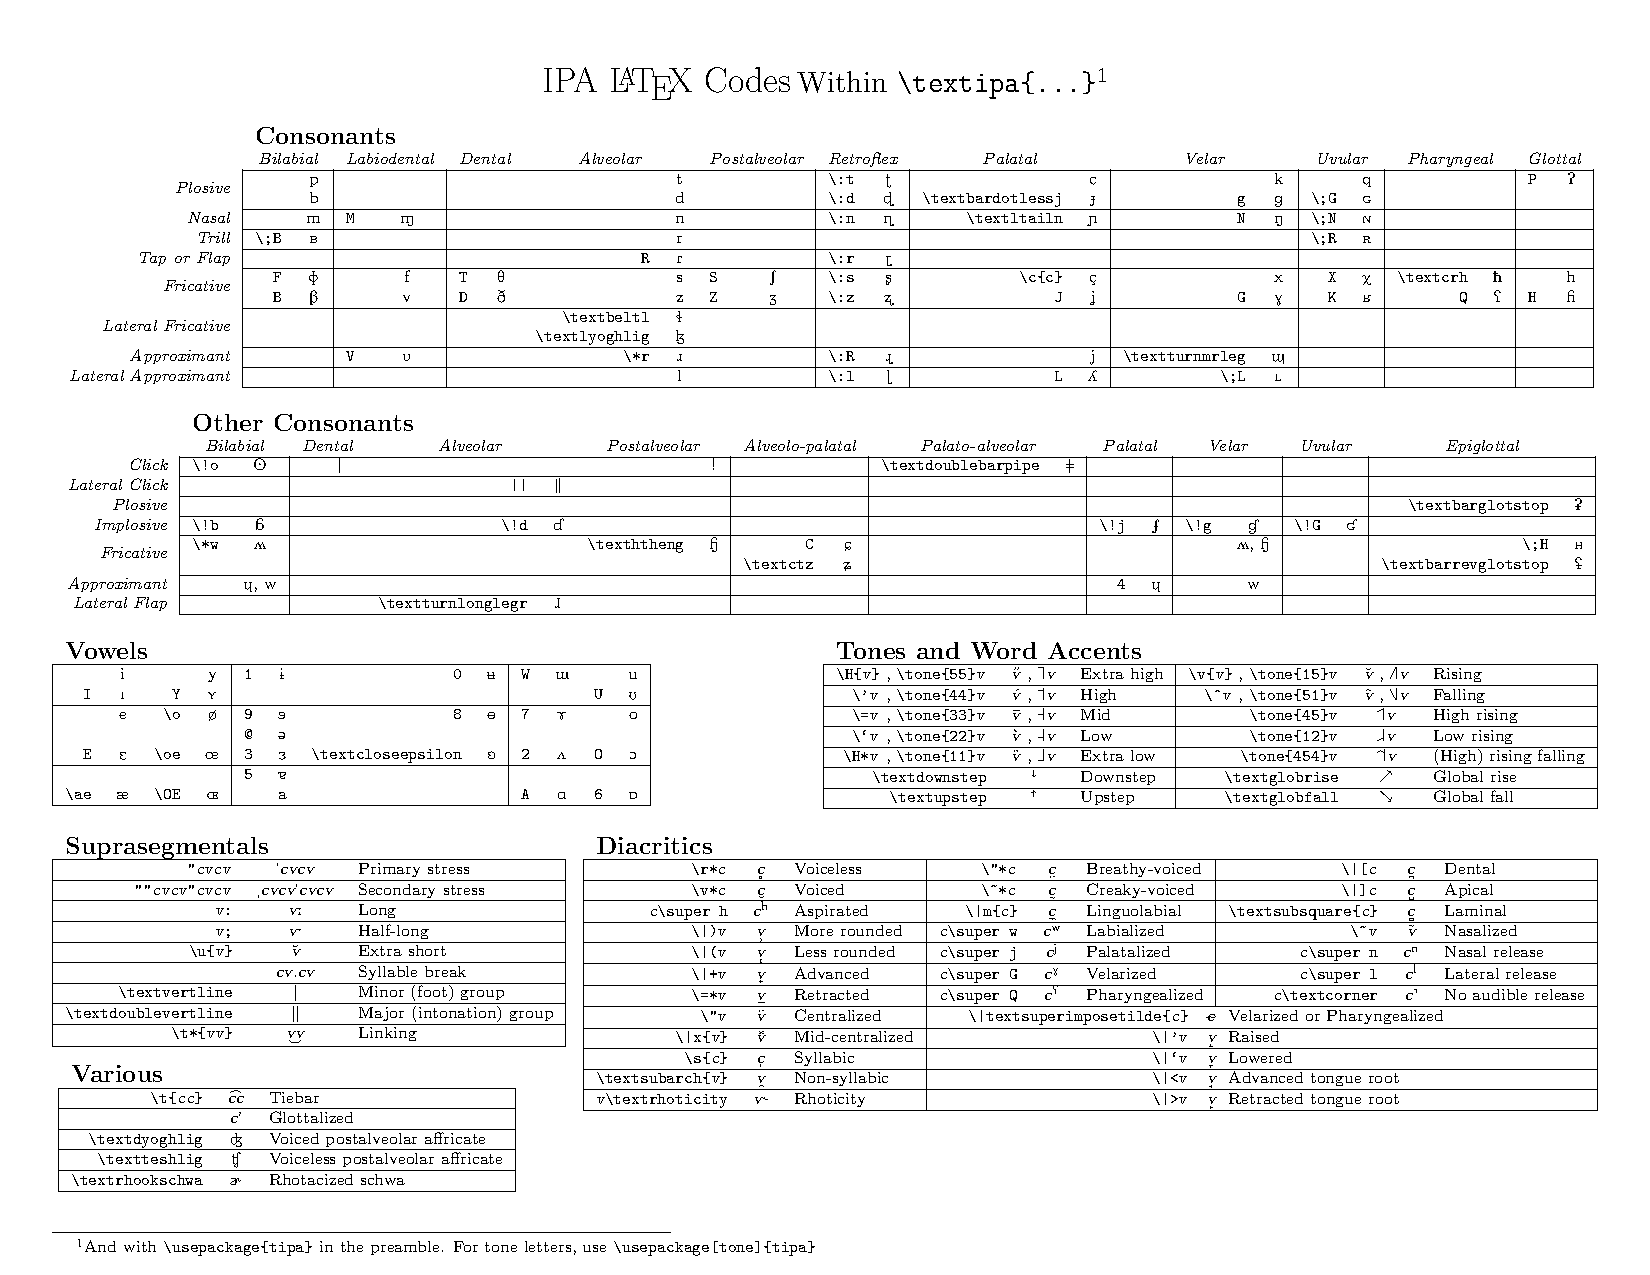
\includegraphics[width=0.7\textwidth,height=0.9\textheight,keepaspectratio]
                     {figures/tipachart_mod.pdf}
  %\caption{Tabela IPA.}
\end{figure}
\end{frame}


\begin{frame}[fragile]
\frametitle{Linguística}
\framesubtitle{Regras fonológicas}
  \scriptsize
  \begin{verbatim}
\usepackage{phonrule}
  
\phonb{\phonfeat{+stop \\ +consonant \\ +alveolar} }{[\textipa{R}]}
{\phonfeat{+vowel \\ +stressed} }{\phonfeat{+vowel \\ +stressed} }
  \end{verbatim}

  \begin{fmpage}{\textwidth}
\phonb{\phonfeat{+stop \\ +consonant \\ +alveolar} }{[\textipa{R}]}{\phonfeat{+vowel \\ +stressed} }{\phonfeat{+vowel \\ +stressed} }
  \end{fmpage}

\end{frame}


\begin{frame}[fragile]
\frametitle{Linguística}
\framesubtitle{Árvores sintáticas}
  \scriptsize
  \begin{columns}[c]
  \column{.5\textwidth}
  \begin{verbatim}
\usepackage{qtree}

\begin{center}
\Tree [.S [.NP LaTeX ] [.VP [.V is ] 
  [.NP fun ] ] ]
\end{center}
  \end{verbatim}
  \column{.5\textwidth}
  \begin{fmpage}{\textwidth}
\begin{center}
\Tree [.S [.NP LaTeX ] [.VP [.V is ] [.NP fun ] ] ]
\end{center}
  \end{fmpage}
  \end{columns}
\end{frame}

\begin{frame}[fragile]
\frametitle{Linguística}
\framesubtitle{Árvore de dependência}

  \begin{fmpage}{\textwidth}
   \begin{dependency}[theme = simple]
   \begin{deptext}[column sep=1em]
      A \& hearing \& is \& scheduled \& on \& the \& issue \& today \& . \\
   \end{deptext}
   \deproot{3}{ROOT}
   \depedge{2}{1}{ATT}
   \depedge[edge start x offset=-6pt]{2}{5}{ATT}
   \depedge{3}{2}{SBJ}
   \depedge{3}{9}{PU}
   \depedge{3}{4}{VC}
   \depedge{4}{8}{TMP}
   \depedge{5}{7}{PC}
   \depedge[arc angle=50]{7}{6}{ATT}
   \end{dependency}
  \end{fmpage}

\end{frame}



\begin{frame}[allowframebreaks,fragile]
\frametitle{siunitx}

O pacote \texttt{siunitx} é utilizado para formatação de texto com quantidades físicas de maneira consistente no texto.

\begin{LTXexample}
\num{12345,67890}  \\
\num{.3e45}        \\
\num{0.123}   \\
\num{0,1234}  \\
\num{3.45d-4} \\
\num{3.4567e-6} 
\end{LTXexample}

\framebreak

\begin{LTXexample}
\num{1.23456}     \\
\num{14.23}      \\
\sisetup{round-mode = places, round-precision = 3}%
\num{1.23456}     \\
\num{14.23}      \\
\end{LTXexample}

\framebreak

\begin{LTXexample}
\begin{table}\caption{Uso tabela sem o pacote \texttt{siunitx}.}
\begin{tabular}{l}
\toprule{Some Values} \\
\midrule 
2.3456 \\ 34.2345 \\ -6.7835 \\ 90.473  \\ 5642.5    \\ 1.2e3 \\ e4  \\
\bottomrule
\end{tabular}
\end{table}
\end{LTXexample}

\framebreak 

\begin{LTXexample}
\begin{table}\caption{Standard behaviour of the \texttt{S} column type.%
\label{tab-S-standard}}
\begin{tabular}{@{}S@{}}
\toprule{Some Values} \\
\midrule 
2.3456 \\ 34.2345 \\ -6.7835 \\ 90.473  \\ 5642.5    \\ 1.2e3 \\ e4  \\
\bottomrule
\end{tabular}
\end{table}
\end{LTXexample}



\end{frame}


\section{Dados}

\begin{frame}
\frametitle{Dataset}

Conjunto de dados (\emph{dataset}) é uma coleção de dados tabulados.

\vspace{3ex}
Os \emph{dataset} podem estar armazenados digitalmente em diferentes formatos.
\begin{itemize}
\item banco de dados (conjunto de dados relacionados);
\item arquivo texto (estruturados ou não);
\item XML;
\item CSV;
\item JSON;
\item XLS, XLSX, ODS;
\item etc
\end{itemize}

\end{frame}



\begin{frame}[allowframebreaks]
\frametitle{Dados públicos}
Brasileiros:
\begin{itemize}
\item IPEA DATA: \url{http://www.ipeadata.gov.br/}
\item IBGE: \url{https://www.ibge.gov.br/}
\item Banco de Informações Econômicas e Financeiras do Banco Central: \url{https://www3.bcb.gov.br/sgspub/localizarseries/localizarSeries.do?method=prepararTelaLocalizarSeries}
\item Datasus: \url{http://datasus.saude.gov.br/}
\item Portal da transparência: \url{http://transparencia.gov.br/}
\item Polícia federal - Ministério da justiça e segurança pública: \url{http://www.pf.gov.br/institucional/acessoainformacao/acesso-a-informacao}
\item Ministério da Cultura: \url{http://sistemas.cultura.gov.br/comparar/salicnet/salicnet.php}
\item Portal brasileiro de dados abertos: \url{http://dados.gov.br/dataset}
\end{itemize}

Estrangeiros:
\begin{itemize}
\item UCI Machine Learning Repository Center para Machine Learning e Sistemas inteligentes: \url{https://archive.ics.uci.edu/ml/datasets.php}
\item Kaggle: \url{https://www.kaggle.com/datasets}
\item Quandl: Financial, Economic and Alternative Data: \url{https://www.quandl.com/}
\item Copa KDD - Arquivos da competição Data Mining e Knowledge Discovery: \url{https://www.kdd.org/kdd-cup}
\item Data Driven Datasets onde a ciência de dados pode ser usada para criar um impacto social: \url{https://www.drivendata.org/}
\item Dados sobre as cidades americanas: \url{http://datasf.org}
\item Governo dos EUA: \url{https://www.data.gov/}
\item Dados do Governo do Canadá: \url{http://open.canada.ca}
\item Dados do Governo do Reino Unido: \url{https://data.gov.uk}
\item Dados da União Europeia: \url{http://open-data.europa.eu/en/data}
\item Censo dos EUA: \url{http://www.census.gov}
\item Google AI: \url{https://ai.google/tools/datasets/}
\item OCDE: \url{http://stats.oecd.org/Index.aspx}
\item Time Series Data Library: \url{https://robjhyndman.com/TSDL/}
\item Macroeconomic Time Series: \url{https://fgn.unisg.ch/eumacro/macrodata/macroeconomic-time-series.html}
\item NOAA - National Environmental Satellite. \url{Data and Information Center: https://www.ngdc.noaa.gov/stp/stp.html}
\item Financial Data Finder: \url{https://fisher.osu.edu/academic-departments/department-finance The Ohio State University}
\item Repository of time series data: \url{http://www.stats.uwo.ca/faculty/aim/epubs/mhsets/}
\item NASA: \url{https://data.giss.nasa.gov/}
\item U.S. Department of Labor (Bureau of Labor Statistics): \url{https://www.bls.gov/data/}
\item ECONSTATS - Global Economic Data: \url{http://www.econstats.com/}
\item The National Bureau of Economic Research: \url{http://www.nber.org/data/}
\item Economagic.com: Economic Time Series Page: \url{http://www.economagic.com/}
\item Time Series Modelling of Water Resources and Environmental Systems: \url{http://www.stats.uwo.ca/faculty/aim/1994Book/default.htm}
\item Dados do Banco Mundial: \url{http://data.worldbank.org}
\item Dados sobre a saúde: \url{http://www.healthdata.gov}
\item Dados públicos da Amazon: \url{http://aws.amazon.com/datasets}
\item Dados sobre diversos países (incluindo o Brasil): \url{http://knoema.com}
\item Dados sobre diversas áreas de negócio e finanças: \url{https://www.quandl.com}
\item Google Trends: \url{https://www.google.com/trends}
\item Google Finance: \url{https://www.google.com/finance}
\item Gapminder: \url{http://www.gapminder.org/data}
\item Dados sobre milhões de músicas: \url{https://aws.amazon.com/datasets/million-song-dataset}
\item Dados sobre os mais diversos assuntos: \url{http://www.freebase.com}
\item DBpedia: \url{http://wiki.dbpedia.org/}
\item Open Data Monitor: \url{http://opendatamonitor.eu}
\item Open Data Network: \url{http://www.opendatanetwork.com}
\item R Datasets: \url{http://www.stats4stem.org/data-sets.html}
\item R Dataset packages Datasets: \url{http://www.statsci.org/datasets.html}
\item Portal de Estatística: \url{http://www.sttista.com}
\item Data 360: \url{http://www.data360.org}
\item Reconhecimento de Faces: \url{http://www.face-rec.org/databases}
\item Stanford Large Network Dataset Collection: \url{http://snap.stanford.edu/data}
\item Datahub: \url{http://datahub.io/dataset}
\item nlp-datasets: \url{https://github.com/niderhoff/nlp-datasets}
\item paperswithcode: \url{https://www.paperswithcode.com/datasets}
\end{itemize}

Lista criada por Fellipe Gomes (\url{https://gomesfellipe.github.io/itemized/item2/}).
\end{frame}





\section{Elementos flutuantes}

\begin{frame}
\frametitle{Elementos flutuantes}
\begin{itemize}
\item figuras
\item tabelas
\item listagens e códigos
\end{itemize}

\vspace{3ex}
Não utilize referências como:  `veja a figura abaixo'.
\end{frame}

\subsection{Tabelas}

\begin{frame}
\frametitle{Tabelas}
Tabelas convêm informação em forma visual.

%Uma tabela é um arranjo de células organizadas em colunas verticais e linhas horizontais.
%As células são elementos mínimos indivisíveis. Dependendo da necessidade, as células podem
%ser mescadas, expandindo assim ao longo de linhas (\verb|\multirow|) ou colunas (\verb|\multicolumn|). 
\vspace{9ex}

\centering
\begin{tabular}{ l c r }
  1 & 2 & 3 \\
  4 & 5 & 6 \\
  7 & 8 & 9 \\
\end{tabular}
\end{frame}


\begin{frame}
\frametitle{Utilize tabelas apenas quando necessário}
\begin{table}[h]
\caption{\label{tab-receita}Receita Coffee Porter (OG: 1,055, FG: 1,012, ABV: 5,6\%, COR: 40, IBU: 27).}
\begin{tabular}{|l|l|l|}
\hline
	& quantidade & ingrediente \\
\hline
\multirow{4}{*}{brassagem} & 3,0 kg & Dry Brew Extrato de Malte \\
	& 0,5 kg & Malte Cara Gold \\
	& 0,4 kg & Malte Chocolate \\
	& 0,3kg & Cevada Torrada \\
\hline 
\multirow{2}{*}{Fervura} & 25g & Target @30min \\
	& 20g & Fuggles @15min \\
\hline
\multirow{2}{*}{Fermentação} & \multirow{2}{*}{1} & Levedura Levteck American Ale \\
	& & 10 dias @ 18C, 7 dias @ 5C \\
\hline
\multirow{2}{*}{envase} & 300ml & Café \\
	&  5g/L & primming \\
\hline
\end{tabular}
\end{table}
\end{frame}

\begin{frame}
\frametitle{Utilize tabelas apenas quando necessário}
\textbf{Receita Coffee Porter}

{\small características: \\OG: 1,055, FG: 1,012, ABV: 5,6\%, COR: 40, IBU: 27}
\begin{description}
\item[brassagem] 
	\begin{itemize}
	\item[--] 3,0 kg Dry Brew Extrato de Malte
	\item[--] 0,5 kg Malte Cara Gold
	\item[--] 0,4 kg Malte Chocolate
	\item[--] 0,3kg Cevada Torrada
	\end{itemize}
\item[fervura]
	\begin{itemize}
	\item[--] 25g Target @30min
	\item[--] 20g Fuggles @15min
	\end{itemize}
\item[fermentação]
	\begin{itemize}
	\item[--] Levedura Levteck American Ale - 10 dias @ 18C, 7 dias @ 5C
	\end{itemize}
\item[envase]
	\begin{itemize}
	\item[--] 300ml de Café
	\item[--] primming: 5g/L
	\end{itemize}
\end{description}
\end{frame}


\begin{frame}[fragile,allowframebreaks]
\frametitle{Tabelas em \LaTeX{}}
\begin{lstlisting}[language=tex, label=lst-tabela, caption={Exemplo de documento em \LaTeX{}}, postbreak=\mbox{$\hookrightarrow$\space}, basicstyle=\fontsize{8}{10}\selectfont\ttfamily]
\begin{tabular}{ l c r }
  1 & 2 & 3 \\
  4 & 5 & 6 \\
  7 & 8 & 9 \\
\end{tabular}
\end{lstlisting}

Definição: \verb|\begin{tabular}[pos]{table spec}|

Onde \texttt{table spec} especifica o alinhamento de cada coluna.

\begin{description}
\item[l] esquerda (\emph{left})
\item[c] centralizado (\emph{centered})
\item[r] direita (\emph{right})
\item[p] parágrafo, deve-se utilizar a sintaxe \verb|p{'width'}| (\emph{paragraph}) 
\item[|] linha vertical
\end{description}

\vspace{3ex}
Definição de múltiplas colunas: \verb|*{num}{str}|

Exemplo: \verb|\begin{tabular}{l*{6}{c}r}|

\framebreak

\vspace{3ex}
Células podem ser mescladas: \verb|\multirow| ou \verb|\multicolumn|.


Sintaxe do comando \verb|\multicolumn|: \\
\verb|\multicolumn{num_cols}{alignment}{contents}|

\begin{description}
\item[num\_cols] número de colunas subsequentes que serão mescladas
\item[alignment] opções de alinhamento \texttt{l, c, r, p}
\item[contents] conteúdo da célula
\end{description}

\framebreak

Sintaxe do comando \verb|\multirow|: \\
\verb|\multirow{num_rows}{width}{contents}|

\begin{description}
\item[num\_rows] número de linhas que serão mescladas
\item[width] largura do texto. O valor \texttt{*} indica a largura natural e \texttt{=} indica a largura da coluna
\end{description}

\end{frame}


\begin{frame}[allowframebreaks,fragile]
\frametitle{Células de múltiplas colunas}

\lstinputlisting[language=tex, label=lst-ex-multicols, postbreak=\mbox{$\hookrightarrow$\space}, basicstyle=\fontsize{8}{10}\selectfont\ttfamily]{examples/multicol.tex}
\begin{table}[ht]
\caption{Multi-column table}
\begin{center}
\begin{tabular}{cc}
    \hline
    \multicolumn{2}{c}{Multi-column}\\
    X&X\\
    \hline
\end{tabular}
\end{center}
\label{tab:multicol}
\end{table}


\end{frame}

\begin{frame}[allowframebreaks,fragile]
\frametitle{Células de múltiplas linhas}

\lstinputlisting[language=tex, label=lst-ex-multicols, postbreak=\mbox{$\hookrightarrow$\space}, basicstyle=\fontsize{8}{10}\selectfont\ttfamily]{examples/multirow.tex}
%\usepackage{multirow} % include in document preamble
\begin{table}[ht]
\caption{Multi-row table}
\begin{center}
\begin{tabular}{cc}
    \hline
    \multirow{2}{*}{Multirow}&X\\
    &X\\
    \hline
\end{tabular}
\end{center}
\label{tab:multicol}
\end{table}


\end{frame}





\begin{frame}
\frametitle{Tabelas}
\centering
\scriptsize
\begin{table}[h]
\csvreader[tabular=|l|l|,
    table head=\hline \bfseries mês & \bfseries gás (R\$),
    late after head=\\\hline\hline,
    late after line=\\\hline,
    filter={\value{csvrow}<18},
    ]%
    {/home/leoca/docs/ape/lodz/consumo/consumo.csv}%
    {mes=\mes,gas=\gas}% use head of csv as column names
    {\mes & \gas}% specify your coloumns here
\caption{\label{tab-example01}Valor gasto mensalmente com gás.}
\end{table}
\end{frame}

\begin{frame}
\frametitle{Tabelas}
\centering
\scriptsize
\begin{table}[h]
\csvreader[tabular=|l|l|,
    before table=\rowcolors{2}{red!25}{yellow!50},
    table head=\hline\rowcolor{red!50!black}\color{white}\bfseries mês & \color{white}\bfseries gás (R\$),
    late after head=\\\hline\hline,
    late after last line=\\\hline,
    filter={\value{csvrow}<18},
    ]%
    {/home/leoca/docs/ape/lodz/consumo/consumo.csv}%
    {mes=\mes,gas=\gas}% use head of csv as column names
    {\mes & \gas}% specify your coloumns here
\caption{\label{tab-example02}Valor gasto mensalmente com gás.}
\end{table}
\end{frame}



\begin{frame}
\frametitle{Tabelas}
\centering
\scriptsize
\begin{table}[h]
\csvstyle{mystyle}{
    tabular=lH,
    head to column names,
    table head=\toprule {mês} & {gás (R\$)} \\\midrule,
    table foot=\bottomrule,
    filter={\value{csvrow}<18}
}
\csvreader[mystyle]{/home/leoca/docs/ape/lodz/consumo/consumo.csv}{}{\mes & \gas}
\caption{\label{tab-example03}Valor gasto mensalmente com gás.}
\end{table}
\end{frame}

\begin{frame}[fragile]
\frametitle{Código utilizado na tabela anterior}
\begin{lstlisting}[language=tex, label=lst-tabela, caption={Tabela gerada a partir de um arquivo CSV. Pacotes utilizados: csvsimple e booktabs.}, postbreak=\mbox{$\hookrightarrow$\space}, basicstyle=\fontsize{8}{10}\selectfont\ttfamily]
\csvstyle{mystyle}{
    tabular=lH,
    head to column names,
    table head=\toprule {mês} & {gás (R\$)} \\\midrule,
    table foot=\bottomrule,
    filter={\value{csvrow}<18}
}
\csvreader[mystyle]{consumo.csv}{}{\mes & \gas}
\end{lstlisting}
\end{frame}


\begin{frame}
\frametitle{Tabelas}
\centering
\scriptsize
\begin{table}[h]
\csvstyle{mystyle}{
    tabular=lH,
    head to column names,
    table head= {mês} & {gás (R\$)} \\\midrule,
    filter={\value{csvrow}<18}
}
\csvreader[mystyle]{/home/leoca/docs/ape/lodz/consumo/consumo.csv}{}{\mes & \gas}
\caption{\label{tab-example03}Valor gasto mensalmente com gás.}
\end{table}
\end{frame}



\begin{frame}
\frametitle{Comparação entre duas tabelas}
\begin{figure}[htbp]
\begin{minipage}[t]{0.47\textwidth}
\centering
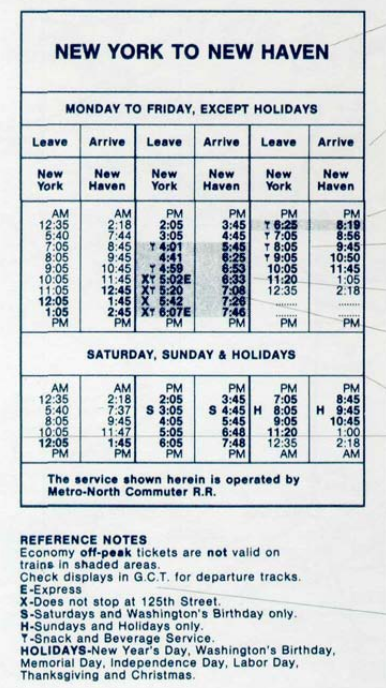
\includegraphics[width=0.64\linewidth,height=0.7\textheight,keepaspectratio]{figures/timetable01.png}
\subcaption{Design ruim.}
\end{minipage}
\hfill
\begin{minipage}[t]{0.47\textwidth}
\centering
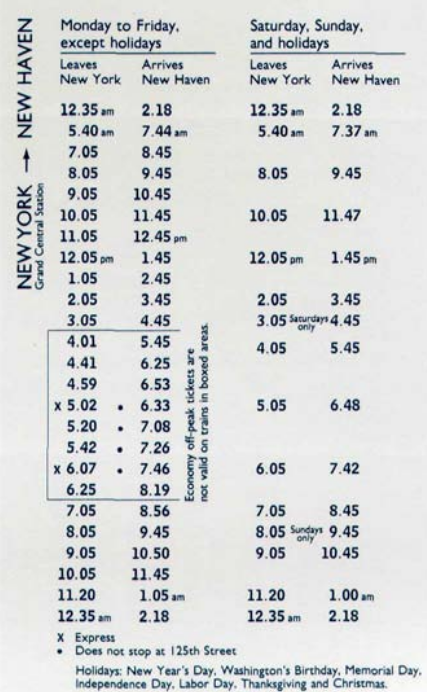
\includegraphics[width=0.7\linewidth,height=0.7\textheight,keepaspectratio]{figures/timetable02.png}
\subcaption{Bom design.}
\end{minipage}
\caption{Tabelas com horários do trem \cite{tufte_envisioning_1990}.}
\end{figure}
% pg105 - Envisioning Information, Edward R. Tufte
% bad design: 
% - direction of the train is not clear
% - repeated headings
% - zig-zag reading
% - poor usege of empty spaces
\end{frame}

\begin{frame}[fragile,allowframebreaks]
\frametitle{stargazer (R)}
\framesubtitle{\emph{Well-Formatted Regression and Summary Statistics Tables}}

\emph{stargazer} é um pacote em R para produzir tabelas bem formatadas em \LaTeX{},
HTML/CSS e ASCII.

\url{https://cran.r-project.org/web/packages/stargazer/}


\begin{lstlisting}[language=R, label=lst-stargazer, caption={Exemplos de utilização do stargazer}, postbreak=\mbox{$\hookrightarrow$\space}, basicstyle=\fontsize{8}{10}\selectfont\ttfamily]
library(stargazer)
stargazer(attitude)
\end{lstlisting}

O resultado é exibido na listagem \ref{lst-ex-stargazer} e na tabela \ref{tab-ex-stargazer}.

\lstinputlisting[language=tex, label=lst-ex-stargazer, postbreak=\mbox{$\hookrightarrow$\space}, basicstyle=\fontsize{8}{10}\selectfont\ttfamily]{ex-stargazer.tex}

\framebreak
\begin{table}[!htbp] \centering 
  \caption{Exemplo gerado pelo \texttt{stargazer} usando o dataframe \texttt{attitude}.} 
  \label{tab-ex-stargazer} 
\begin{tabular}{@{\extracolsep{5pt}}lccccccc} 
\\[-1.8ex]\hline 
\hline \\[-1.8ex] 
Statistic & \multicolumn{1}{c}{N} & \multicolumn{1}{c}{Mean} & \multicolumn{1}{c}{St. Dev.} & \multicolumn{1}{c}{Min} & \multicolumn{1}{c}{Pctl(25)} & \multicolumn{1}{c}{Pctl(75)} & \multicolumn{1}{c}{Max} \\ 
\hline \\[-1.8ex] 
rating & 30 & 64.633 & 12.173 & 40 & 58.8 & 71.8 & 85 \\ 
complaints & 30 & 66.600 & 13.315 & 37 & 58.5 & 77 & 90 \\ 
privileges & 30 & 53.133 & 12.235 & 30 & 45 & 62.5 & 83 \\ 
learning & 30 & 56.367 & 11.737 & 34 & 47 & 66.8 & 75 \\ 
raises & 30 & 64.633 & 10.397 & 43 & 58.2 & 71 & 88 \\ 
critical & 30 & 74.767 & 9.895 & 49 & 69.2 & 80 & 92 \\ 
advance & 30 & 42.933 & 10.289 & 25 & 35 & 47.8 & 72 \\ 
\hline \\[-1.8ex] 
\end{tabular} 
\end{table} 



\end{frame}


\begin{frame}[fragile,allowframebreaks]
\frametitle{Octave to \LaTeX{}}

\begin{lstlisting}[language=Octave, label=lst-octave-matrix, caption={Gerando a matriz em \LaTeX{} a partir do GNU Octave}, postbreak=\mbox{$\hookrightarrow$\space}, basicstyle=\fontsize{8}{10}\selectfont\ttfamily]
A = magic(8);
strcat("\\begin{bmatrix}\n",strrep(strrep(mat2str(A)," "," & "),";","\\\\\n")(2:end-1),"\n\\end{bmatrix}\n")
\end{lstlisting}

$
\begin{bmatrix}
64 & 2 & 3 & 61 & 60 & 6 & 7 & 57\\
9 & 55 & 54 & 12 & 13 & 51 & 50 & 16\\
17 & 47 & 46 & 20 & 21 & 43 & 42 & 24\\
40 & 26 & 27 & 37 & 36 & 30 & 31 & 33\\
32 & 34 & 35 & 29 & 28 & 38 & 39 & 25\\
41 & 23 & 22 & 44 & 45 & 19 & 18 & 48\\
49 & 15 & 14 & 52 & 53 & 11 & 10 & 56\\
8 & 58 & 59 & 5 & 4 & 62 & 63 & 1
\end{bmatrix}

$

\begin{lstlisting}[language=Octave, label=lst-octave-table, caption={Gerando uma tabela em \LaTeX{} a partir do GNU Octave}, postbreak=\mbox{$\hookrightarrow$\space}, basicstyle=\fontsize{8}{10}\selectfont\ttfamily]
A = magic(8);
strcat("\\begin{table}[!htbp]\\centering\n\\caption{}\n\\label{}\n\\begin{tabular}{",repmat('l',1,size(A,2)),"}\n\\hline\n",strrep(strrep(mat2str(A)," "," & "),";","\\\\\n")(2:end-1),"\\\\\n\\hline\n\\end{tabular}\n\\end{table}")
\end{lstlisting}

\framebreak
\begin{table}[!htbp]\centering
\caption{Tabela gerada através do GNU Octave.}
\label{tbl-ex-octave}
\begin{tabular}{llllllll}
\hline
64 & 2 & 3 & 61 & 60 & 6 & 7 & 57\\
9 & 55 & 54 & 12 & 13 & 51 & 50 & 16\\
17 & 47 & 46 & 20 & 21 & 43 & 42 & 24\\
40 & 26 & 27 & 37 & 36 & 30 & 31 & 33\\
32 & 34 & 35 & 29 & 28 & 38 & 39 & 25\\
41 & 23 & 22 & 44 & 45 & 19 & 18 & 48\\
49 & 15 & 14 & 52 & 53 & 11 & 10 & 56\\
8 & 58 & 59 & 5 & 4 & 62 & 63 & 1\\
\hline
\end{tabular}
\end{table}


\framebreak
\lstinputlisting[language=tex, label=lst-ex-octave-table, postbreak=\mbox{$\hookrightarrow$\space}, basicstyle=\fontsize{8}{10}\selectfont\ttfamily]{examples/octave-table.tex}

\end{frame}



\begin{frame}
\frametitle{Dicas}
\begin{itemize}
\item \hrefcolor{https://www.tablesgenerator.com/}{tables generator}
\item \hrefcolor{https://www.latex-tables.com/}{latex tables}
\end{itemize}
\end{frame}




\begin{frame}
Sugestões de leitura: 
\vspace{2ex}

\hrefcolor{https://en.wikibooks.org/wiki/LaTeX/Tables}{Wikibooks - \LaTeX{} / Tables}
\vspace{2ex}

\fullcite{chicago_2017}
\end{frame}


\subsection{Figuras}

\begin{frame}
\epigraph{I call our world Flatland, not because we call it so, 
but to make its nature clearer to you, my happy readers, 
who are privileged to live in space.}{Edwin A. Abbott, Flatland: A Romance of Many Dimensions}
\end{frame}


\begin{frame}
\frametitle{Figuras}
Figuras possuem uma grande potencial para levar informação de forma simples ao leitor.
Podem evidenciar padrões, tendências e anomalias, constâncias ou variações. 
Devem ser utilizadas com parcimônia e muito bem elaboradas.

\vspace{3ex}
Figuras são elementos flutuantes e que devem ser capazes de passar uma mensagem sozinhas.
\end{frame}


\begin{frame}
\frametitle{xkcd}
\begin{figure}[h]
\centering
\includegraphics[width=0.6\textwidth,height=0.6\textheight,keepaspectratio]{figures/scientific_paper_graph_quality.png}
\caption{Scientific Paper Graph Quality (\url{https://xkcd.com/1945/}).}
\label{fig-scientific_paper_graph_quality}
\end{figure}
\end{frame}

\begin{frame}
\frametitle{Eventos na história da visualização de dados}
\begin{figure}[h]
\centering
\includegraphics[width=0.8\textwidth,height=0.8\textheight,keepaspectratio]{figures/hist_data_visualization.png}
\caption{Retirada de \textcite{Friendly2008}.}
\label{fig-hist_data_visualization}
\end{figure}
\end{frame}


\begin{frame}
\frametitle{Figuras}

Florence Nightingale liderou uma pequena equipe de enfermeiras a Istambul em
1854 para ajudar no cuidado dos soldados britânicos que lutaram na guerra da
Crimeia. Seus gráficos convenceram os grandes e os bons de que as mortes devido
à sujeira e ao saneamento deficiente poderiam ser evitadas - salvando inúmeras
vidas.

\vspace{2ex}
\fullcite{harford_florence}

\vspace{1ex}
\hrefcolor{https://99percentinvisible.org/episode/florence-nightingale-data-viz-pioneer/}{Florence Nightingale: Data Viz Pioneer, 99percentinvisible.org}

\hrefcolor{https://en.wikipedia.org/wiki/Florence_Nightingale}{Florence Nightingale, Wikipedia}

\hrefcolor{https://www.youtube.com/watch?v=VTdVPNvwULM}{Nightingale Diagrams, Numberphile}

\hrefcolor{https://www.youtube.com/watch?v=sNppKQh0xPo}{What would Florence Nightingale make of big data?, BBC Ideas}
\end{frame}
% Coxcomb plots and 'spiecharts' in R
% https://rpubs.com/RobinLovelace/11641

\begin{frame}
\frametitle{Florence Nightingale}
\begin{figure}[h]
 \centering
 \includegraphics[width=0.8\textwidth,height=0.75\textheight,keepaspectratio]{figures/nightingale-mortality.jpg}
 \caption{Diagrama de mortalidade feito por Florence Nightingale.}
 \label{fig-nightingale-mortality}
\end{figure}
\end{frame}
\note{
O gráfico proposto por Florence Nightingale evidencia as mortes pelas áreas, sendo
dividas por três causas: doenças infectocontagiosas (azul), ferimentos (vermelho) e outras (preto).
O gráfico da direito apresenta o período durante a guerra antes da adoção de medidas sanitárias
e o gráfico da esquerda evidencia o período após a adoções de medidas sanitárias. 
O tempo é visto no sentido horário e a posição no gráfico facilita a comparação dos
meses em anos diferentes.
}






\begin{frame}[allowframebreaks]
\frametitle{Exemplo 1 - \emph{Storytelling with Data}}
\begin{figure}[h]
 \centering
 \includegraphics[width=0.8\textwidth,height=0.6\textheight,keepaspectratio]{figures/storytelling_data_ex01a.png}
 \caption{Preço médio de venda de produtos ao longo dos anos \cite{knaflic_storytelling_2015}.}
 \label{fig-storytelling_data_ex01a}
\end{figure}
\framebreak
\begin{figure}[h]
 \centering
 \includegraphics[width=0.8\textwidth,height=0.7\textheight,keepaspectratio]{figures/storytelling_data_ex01b.png}
 \caption{Preço médio de venda de produtos ao longo dos anos \cite{knaflic_storytelling_2015}.}
 \label{fig-storytelling_data_ex01b}
\end{figure}
\end{frame}


\begin{frame}[allowframebreaks=1]
\frametitle{Exemplo 2 - \emph{Storytelling with Data}}
\begin{figure}[h]
 \centering
 \includegraphics[width=0.8\textwidth,height=0.6\textheight,keepaspectratio]{figures/storytelling_data_ex02a.png}
 \caption{Volume de tickes recebidos e processados. \cite{knaflic_storytelling_2015}.}
 \label{fig-storytelling_data_ex02a}
\end{figure}
\framebreak
\begin{figure}[h]
 \centering
 \includegraphics[width=0.8\textwidth,height=0.7\textheight,keepaspectratio]{figures/storytelling_data_ex02b.png}
 \caption{Volume de tickes recebidos vs. processados. O descolamento evidencia a necessidade de contratação. \cite{knaflic_storytelling_2015}.}
 \label{fig-storytelling_data_ex02b}
\end{figure}
\end{frame}

\begin{frame}[allowframebreaks=1]
\frametitle{Exemplo 3 - \emph{Storytelling with Data}}
\begin{figure}[h]
 \centering
 \includegraphics[width=0.8\textwidth,height=0.6\textheight,keepaspectratio]{figures/storytelling_data_ex03a.png}
 \caption{Resultado da pesquisa de opinião sobre ciências. \cite{knaflic_storytelling_2015}.}
 \label{fig-storytelling_data_ex03a}
\end{figure}
\framebreak
\begin{figure}[h]
 \centering
 \includegraphics[width=0.7\textwidth,height=0.6\textheight,keepaspectratio]{figures/storytelling_data_ex03b.png}
 \caption{Resultado da pesquisa de opinião sobre ciências. \cite{knaflic_storytelling_2015}.}
 \label{fig-storytelling_data_ex03b}
\end{figure}
\end{frame}


\begin{frame}[allowframebreaks,fragile]
\frametitle{Limitações de alguns gráficos}

\begin{lstlisting}[language=Octave, label=lst-pie-ex, caption={Exemplo de limitações do gráficos.}, postbreak=\mbox{$\hookrightarrow$\space}, basicstyle=\fontsize{8}{10}\selectfont\ttfamily]
x = [0.07 0.12 0.08 0.13 0.075 0.126 0.083 0.135 0.063 0.118]; 
pie(x,strcat('item',strsplit(num2str(1:length(x)))));
print -dsvg piex.svg

lbs=strcat('item',strsplit(num2str(1:length(x))));
[_,idx]=sort(x);
pie(x(idx),lbs(idx)); 

plot(x,'ok','markerfacecolor','k')
set(gca,'Visible','off')
axes('Position',get(gca,'Position'),'XAxisLocation','bottom','YAxisLocation','left', 'Color','none','XTickLabel',get(gca,'XTickLabel'),'YTickLabel',get(gca,'YTickLabel'),'XColor','k','YColor','k','LineWidth',1,'TickDir','out');
print -dsvg piex-dots.svg

plot(x(idx),'ok','markerfacecolor','k');
set(gca,'xtick',[1:length(x)]); set(gca,'xticklabel',lbs(idx));

plot(x(idx),'ok','markerfacecolor','k');
set(gca,'Visible','off')
axes('Position',get(gca,'Position'),'XAxisLocation','bottom','YAxisLocation','left', 'Color','none','XTick',linspace(1/(length(x)),1,length(x)),'XTickLabel',lbs(idx),'YTickLabel',get(gca,'YTickLabel'),'XColor','k','YColor','k','LineWidth',1,'TickDir','out');
print -dsvg piex-dots-order.svg

pie3([0.2 0.2 0.2 0.4],{'','','',''}); view (0,12);
print -dsvg pie3d.svg
\end{lstlisting}

\begin{figure}[h]
 \centering
  \includegraphics[width=0.6\textwidth,height=0.6\textheight,keepaspectratio]{figures/piex.pdf}
 \caption{Gráfico pizza gerado pelo código na lista \ref{lst-pie-ex}. Qual item é maior? e menor?}
 \label{fig-piex}
\end{figure}


\begin{figure}[h]
 \centering
  \includegraphics[width=0.8\textwidth,height=0.7\textheight,keepaspectratio]{figures/piex-dots.pdf}
 \caption{Gráfico de pontos gerado pelo código na lista \ref{lst-pie-ex}. É possível distinguir dois grupos.}
 \label{fig-piex2}
\end{figure}

\begin{figure}[h]
 \centering
  \includegraphics[width=0.8\textwidth,height=0.65\textheight,keepaspectratio]{figures/piex-dots-order.pdf}
 \caption{Gráfico de pontos gerado pelo código na lista \ref{lst-pie-ex}. É possível distinguir dois grupos e verificar a ordem de valores dos itens.}
 \label{fig-piex3}
\end{figure}

\begin{quote}
"Pie charts have severe perceptual problems. Experiments in graphical perception have shown
that compared with dot charts, they convey information far
less reliably. But if you want to display some data, and perceiving the information is not so important, then a pie chart
is fine." \cite{becker1996}
\end{quote}

\begin{quote}
"dumb pie chart; the only worse design than a pie chart is several of them,
for then the viewer is asked to compare quantities located in
spatial disarray both within and between pies. ... Given their
low data-density and failure to order numbers along a visual
dimension, pie charts should never be used." \cite{tufte_visual_1999}
\end{quote}

\framebreak

\begin{figure}[h]
 \centering
  \includegraphics[width=0.7\textwidth,height=0.5\textheight,keepaspectratio]{figures/pie3d.pdf}
 \caption{Nada é tão ruim que não possa piorar.}
 \label{fig-pie3d}
\end{figure}

\framebreak

\begin{figure}[h]
 \centering
  \includegraphics[width=0.7\textwidth,height=0.5\textheight,keepaspectratio]{figures/3dbars.pdf}
 \caption{Evite gráficos com 3D desnecessários.}
 \label{fig-3dbars}
\end{figure}

\end{frame}


\begin{frame}[allowframebreaks]
\frametitle{Playfair's Balance-of-Trade}

\begin{figure}[h]
 \centering
  \includegraphics[width=0.7\textwidth,height=0.6\textheight,keepaspectratio]{figures/imports-exports.png}
 \caption{Balanço de comércio.}
 \label{fig-importex1}
\end{figure}

\framebreak

\begin{figure}[h]
 \centering
  \includegraphics[width=0.7\textwidth,height=0.6\textheight,keepaspectratio]{figures/imports-exports_a.png}
 \caption{Balanço de comércio.}
 \label{fig-importex1a}
\end{figure}

\framebreak

\begin{figure}[h]
 \centering
  \includegraphics[width=0.7\textwidth,height=0.6\textheight,keepaspectratio]{figures/imports-exports_b.png}
 \caption{Balanço de comércio.}
 \label{fig-importex1b}
\end{figure}

\framebreak

\begin{figure}[h]
 \centering
  \includegraphics[width=0.7\textwidth,height=0.9\textheight,keepaspectratio]{figures/imports-exports2.png}
 \caption{Balanço de comércio.}
 \label{fig-importex2}
\end{figure}

\end{frame}




\begin{frame}[allowframebreaks,fragile]
\frametitle{Limitações de alguns gráficos}

\begin{lstlisting}[language=Octave, label=lst-y1y2, caption={Onde as curvas $y_1$ e $y_2$ estão mais próximas e mais distantes?}, postbreak=\mbox{$\hookrightarrow$\space}, basicstyle=\fontsize{8}{10}\selectfont\ttfamily]
x = [0.5:0.125:3];
y1 = 1./x.^2; y2 = y1 + 0.6;
plot(x,y1,'-',x,y2,'--'); legend('y_1','y_2');
print -dsvg curvesy1y2.svg
\end{lstlisting}

\begin{figure}[h]
 \centering
  \includegraphics[width=0.7\textwidth,height=0.9\textheight,keepaspectratio]{figures/curvesy1y2.pdf}
 \caption{Diferença entre as curvas.}
 \label{fig-curvesy1y2}
\end{figure}

\end{frame}


\begin{frame}[allowframebreaks,fragile]
\frametitle{Limitações de alguns gráficos}
\begin{lstlisting}[language=Octave, label=lst-y1y2, caption={Onde as curvas $y_1$ e $y_2$ estão mais próximas e mais distantes?}, postbreak=\mbox{$\hookrightarrow$\space}, basicstyle=\fontsize{8}{10}\selectfont\ttfamily]
system('wget https://gist.githubusercontent.com/curran/13d30e855d48cdd6f22acdf0afe27286/raw/0635f14817ec634833bb904a47594cc2f5f9dbf8/worldcities_clean.csv -O /tmp/worldcities.csv')
X = csvread ('/tmp/worldcities.csv');
top100 = X(2:104,5);
id=find(top100==0);
top100(id)=[];
figure; hold on; for i=1:10:100, drawCircle(i-1,top100(i)/top100(end),top100(i)/top100(end)); end; plot([0:99],top100./top100(end),'k-'); hold off; daspect([1 1 1]);
\end{lstlisting}

\begin{figure}[h]
 \centering
  \includegraphics[width=\textwidth,height=0.5\textheight,keepaspectratio]{figures/citiespop.pdf}
 \caption{População das cidades.}
 \label{fig-citiespop}
\end{figure}

\end{frame}


\begin{frame}[allowframebreaks,fragile]
\frametitle{Limitações de alguns gráficos}
\begin{lstlisting}[language=Octave, label=lst-scatters, caption={Gráfico de espalhamento com 3 grupos.}, postbreak=\mbox{$\hookrightarrow$\space}, basicstyle=\fontsize{8}{10}\selectfont\ttfamily]
X1=rand(20,2)+0.25; X2=0.8*rand(20,2)+0.5; X3=0.6*rand(20,2)+0.75;
figure; hold on; scatter(X1(:,1),X1(:,2),40,[0 0 0],'o','filled'); scatter(X2(:,1),X2(:,2),40,[0 0 0],'s','filled'); scatter(X3(:,1),X3(:,2),40,[0 0 0],'v','filled'); hold off;
print -dsvg scatterplot1.svg
figure; hold on; scatter(X1(:,1),X1(:,2),40,[0 0 0],'o','filled'); scatter(X2(:,1),X2(:,2),40,[0.3 0.3 0.3],'s','filled'); scatter(X3(:,1),X3(:,2),40,[0.6 0.6 0.6],'v','filled'); hold off;
print -dsvg scatterplot2.svg
\end{lstlisting}

\framebreak 

\begin{figure}[h]
 \centering
  \includegraphics[width=0.7\textwidth,height=0.7\textheight,keepaspectratio]{figures/scatterplot1.pdf}
 \caption{Gráfico de espalhamento utilizando tipo de elemento para distinguir os grupos.}
 \label{fig-scatterplot1}
\end{figure}


\framebreak

\begin{figure}[h]
 \centering
  \includegraphics[width=0.7\textwidth,height=0.7\textheight,keepaspectratio]{figures/scatterplot2.pdf}
 \caption{Gráfico de espalhamento utilizando também a cor para distinguir os grupos.}
 \label{fig-scatterplot2}
\end{figure}

\end{frame}


\begin{frame}[allowframebreaks,fragile]
\frametitle{Limitações de alguns gráficos}
\begin{lstlisting}[language=Octave, label=lst-scatters, caption={Gráfico de espalhamento com 3 grupos.}, postbreak=\mbox{$\hookrightarrow$\space}, basicstyle=\fontsize{8}{10}\selectfont\ttfamily]
x = [4 11 22 29 38 42 49 7 13 22 31 39 42 49 7 14 23 32 40 43 55 9 15 27 33 40 45 58 10 15 27 33 40 47 66 10 20 28 35 40 48 72 11 21 28 38 42 48 73];
plot(x,0,'ko'); ylim ([-5 5]);
set(gca,'Visible','off')
axes('Position',get(gca,'Position'),'XAxisLocation','bottom','YAxisLocation','left', 'Color','none','XTickLabel',get(gca,'XTickLabel'),'YTickLabel',get(gca,'YTickLabel'),'XColor','k','YColor','k','LineWidth',1,'TickDir','out');
print -dsvg strip1.svg

plot(x,0.125*randn(1,length(x)),'ko'); ylim ([-5 5]);
set(gca,'Visible','off')
axes('Position',get(gca,'Position'),'XAxisLocation','bottom','YAxisLocation','left', 'Color','none','XTickLabel',get(gca,'XTickLabel'),'YTickLabel',get(gca,'YTickLabel'),'XColor','k','YColor','k','LineWidth',1,'TickDir','out');
print -dsvg strip2.svg
\end{lstlisting}

\framebreak

\begin{figure}[h]
 \centering
  \includegraphics[width=0.7\textwidth,height=0.7\textheight,keepaspectratio]{figures/strip1.pdf}
 \caption{Strip plot.}
 \label{fig-strip1}
\end{figure}

\framebreak

\begin{figure}[h]
 \centering
  \includegraphics[width=0.7\textwidth,height=0.7\textheight,keepaspectratio]{figures/strip2.pdf}
 \caption{Strip plot com Jittering - possibilita a visualização de pontos sobrepostos.}
 \label{fig-strip2}
\end{figure}
\end{frame}


\begin{frame}
\frametitle{Razão de aspecto}

\begin{figure}[h]
 \centering
  \includegraphics[width=0.5\textwidth,height=0.7\textheight,keepaspectratio]{figures/sunspots.png}
 \caption{Número de manchas solares ao longo dos anos \cite{robbins_creating_2013}. Razão de aspecto 0.8 (gráfico de cima) e 0.055 (gráfico de baixo).}
 \label{fig-sunspots}
\end{figure}

\end{frame}
\note{
Note como a razão de aspecto influencia na percepção dos altos e baixos no gráfico.
No gráfico de baixo fica evidente a diferença na velocidade de subida e descida.
}


\begin{frame}
\frametitle{Razão de aspecto e referência zero}
\begin{figure}[h]
 \centering
  \includegraphics[width=0.8\textwidth,height=0.7\textheight,keepaspectratio]{figures/carbondioxide.png}
 \caption{Nível de dióxido de carbono na atmosfera \cite{robbins_creating_2013}.}
 \label{fig-carbondioxide}
\end{figure}
\end{frame}


\begin{frame}
\frametitle{Escala logarítmica}
\begin{figure}[h]
 \centering
  \includegraphics[width=0.8\textwidth,height=0.7\textheight,keepaspectratio]{figures/uselogscale.png}
 \caption{Uso da escala logarítmica \cite{robbins_creating_2013}. Os valores dobram a cada dia.}
 \label{fig-uselogscale}
\end{figure}
\end{frame}


\begin{frame}
\frametitle{Eixo y duplo}
\begin{figure}[h]
 \centering
  \includegraphics[width=\textwidth,height=0.7\textheight,keepaspectratio]{figures/dyaxis.png}
 \caption{Uso de eixo y duplo \cite{robbins_creating_2013}.}
 \label{fig-dyaxis}
\end{figure}
Evite usar eixo y duplo. Note como uma má escolha pode levar a uma interpretação errônea.
\end{frame}

\begin{frame}
\frametitle{Variáveis com extensões diferentes}
\begin{figure}[h]
 \centering
  \includegraphics[width=0.9\textwidth,height=0.7\textheight,keepaspectratio]{figures/range.png}
 \caption{Nível sanguíneo \cite{robbins_creating_2013}.}
 \label{fig-range}
\end{figure}
\end{frame}


\begin{frame}[allowframebreaks,fragile]
\frametitle{Dados de crescimento de dentes}
Vamos analisar os dados de crescimento de dente em Porquinho-da-Índia disponíveis no R (\emph{Tooth Growth Data}).
Os dados mostram o crescimento de odontoblasto\footnote{Odontoblasto é um tipo de células colunares responsáveis pela síntese de matriz da pré-dentina.}
em 10 porquinhos-da-índia a 3 dosagens de vitamina C (0.5, 1, e 2 mg) com dois métodos de entrega (suco de laranja (OJ) e ácido ascórbico (VC)).
Os dados apresentam 60 observações de 3 variáveis (tamanho do dente, tipo de suplemento e dosagem).

\vspace{3ex}
\fullcite{crampton_growth_1947}

\begin{lstlisting}[language=R, label=lst-tooth-0, caption={Resumo dos dados.}, postbreak=\mbox{$\hookrightarrow$\space}, basicstyle=\fontsize{8}{10}\selectfont\ttfamily]
> data(ToothGrowth)
> summary(ToothGrowth)
      len        supp         dose      
 Min.   : 4.20   OJ:30   Min.   :0.500  
 1st Qu.:13.07   VC:30   1st Qu.:0.500  
 Median :19.25           Median :1.000  
 Mean   :18.81           Mean   :1.167  
 3rd Qu.:25.27           3rd Qu.:2.000  
 Max.   :33.90           Max.   :2.000  
\end{lstlisting}

\begin{lstlisting}[language=R, label=lst-tooth-1, caption={Gráfico de pontos evidenciando cada amostra.}, postbreak=\mbox{$\hookrightarrow$\space}, basicstyle=\fontsize{8}{10}\selectfont\ttfamily]
> library(ggplot2)
> library(dplyr)
> ggplot(ToothGrowth, aes(x= dose, y= len)) + geom_point(aes(color=supp)) + theme_minimal()
> ggsave('tooth01.pdf')
\end{lstlisting}

\begin{figure}[h]
 \centering
  \includegraphics[width=0.7\textwidth,height=0.7\textheight,keepaspectratio]{figures/tooth01.pdf}
 \caption{Gráfico de pontos evidenciando as amostras. Gerado pelo código na lista \ref{lst-tooth-1}.}
 \label{fig-tooth01}
\end{figure}

\begin{lstlisting}[language=R, label=lst-tooth-2, caption={Sumário dos dados.}, postbreak=\mbox{$\hookrightarrow$\space}, basicstyle=\fontsize{8}{10}\selectfont\ttfamily]
> ToothGrowth %>% group_by(supp,dose) %>% summarize(lenmean=mean(len), lensd=sd(len), count = n())
`summarise()` has grouped output by 'supp'. You can override using the `.groups` argument.
# A tibble: 6 x 5
# Groups:   supp [2]
  supp   dose lenmean lensd count
  <fct> <dbl>   <dbl> <dbl> <int>
1 OJ      0.5   13.2   4.46    10
2 OJ      1     22.7   3.91    10
3 OJ      2     26.1   2.66    10
4 VC      0.5    7.98  2.75    10
5 VC      1     16.8   2.52    10
6 VC      2     26.1   4.80    10
\end{lstlisting}

\framebreak

\begin{lstlisting}[language=R, label=lst-tooth-jitter, caption={Jitter.}, postbreak=\mbox{$\hookrightarrow$\space}, basicstyle=\fontsize{8}{10}\selectfont\ttfamily]
ggplot(ToothGrowth, aes(x= dose, y= len)) + geom_jitter(aes(color=supp), shape=16, position=position_jitter(0.1)) + theme_minimal()
ggsave('tooth-jitter.pdf')
\end{lstlisting}

\begin{figure}[h]
 \centering
  \includegraphics[width=0.7\textwidth,height=0.7\textheight,keepaspectratio]{figures/tooth-jitter.pdf}
 \caption{Gráfico de \emph{jitter} evidenciando as amostras. Gerado pelo código na lista \ref{lst-tooth-jitter}.}
 \label{fig-tooth-jitter}
\end{figure}


\framebreak

\begin{lstlisting}[language=R, label=lst-tooth-3, caption={Box plot.}, postbreak=\mbox{$\hookrightarrow$\space}, basicstyle=\fontsize{8}{10}\selectfont\ttfamily]
library(ggplot2)
ToothGrowth$dose <- as.factor(ToothGrowth$dose)
ggplot(ToothGrowth, aes(x=dose, y=len)) + geom_boxplot() + theme_minimal()
ggsave('tooth02.pdf')
\end{lstlisting}

\begin{figure}[h]
 \centering
  \includegraphics[width=0.7\textwidth,height=0.7\textheight,keepaspectratio]{figures/tooth02.pdf}
 \caption{Diagrama de caixa (\emph{Box plot}). Gerado pelo código na lista \ref{lst-tooth-3}.}
 \label{fig-tooth02}
\end{figure}

\framebreak

\begin{lstlisting}[language=R, label=lst-tooth-4, caption={Box plot.}, postbreak=\mbox{$\hookrightarrow$\space}, basicstyle=\fontsize{8}{10}\selectfont\ttfamily]
ggplot(ToothGrowth, aes(x=dose, y=len)) + geom_boxplot(notch=TRUE, outlier.colour="red", outlier.shape=8, outlier.size=4) + coord_flip() + theme_minimal()
ggsave('tooth03.pdf')
\end{lstlisting}

\begin{figure}[h]
 \centering
  \includegraphics[width=0.7\textwidth,height=0.7\textheight,keepaspectratio]{figures/tooth03.pdf}
 \caption{Diagrama de caixa (\emph{Box plot}). Gerado pelo código na lista \ref{lst-tooth-4}.}
 \label{fig-tooth03}
\end{figure}

\framebreak

\begin{lstlisting}[language=R, label=lst-tooth-5, caption={Box plot.}, postbreak=\mbox{$\hookrightarrow$\space}, basicstyle=\fontsize{8}{10}\selectfont\ttfamily]
ggplot(ToothGrowth, aes(x=dose, y=len, fill=dose)) + geom_boxplot(notch=TRUE, outlier.colour="red", outlier.size=2) + coord_flip() + theme_minimal() + theme(legend.position="bottom")
ggsave('tooth04.pdf')
\end{lstlisting}

\begin{figure}[h]
 \centering
  \includegraphics[width=0.7\textwidth,height=0.7\textheight,keepaspectratio]{figures/tooth04.pdf}
 \caption{Diagrama de caixa (\emph{Box plot}). Gerado pelo código na lista \ref{lst-tooth-5}.}
 \label{fig-tooth04}
\end{figure}

\framebreak

\begin{lstlisting}[language=R, label=lst-tooth-6, caption={Box plot.}, postbreak=\mbox{$\hookrightarrow$\space}, basicstyle=\fontsize{8}{10}\selectfont\ttfamily]
ggplot(ToothGrowth, aes(x=dose, y=len, fill=supp)) + geom_boxplot() + theme_minimal()
ggsave('/tmp/tooth05.pdf')
\end{lstlisting}

\begin{figure}[h]
 \centering
  \includegraphics[width=0.7\textwidth,height=0.7\textheight,keepaspectratio]{figures/tooth05.pdf}
 \caption{Diagrama de caixa (\emph{Box plot}). Gerado pelo código na lista \ref{lst-tooth-6}.}
 \label{fig-tooth05}
\end{figure}

\framebreak

\begin{footnotesize}
Examining Tooth Growth Data in R\\
\url{https://rpubs.com/garedwards/107023}

\begin{quote}
Conclusions and Assumptions

Based off this data we can conclude the following:
\begin{itemize}
\item As dosage increases, tooth length increases regardless of supplement method.
\item At the 0.5 mg and 1.0 mg dosage the OJ supplement method leads to more tooth growth than the VC method.
\item At the 2.0 mg dosage, there is no significant difference between the OJ and VC supplement methods.
\end{itemize}

Assumptions
\begin{itemize}
\item We assume that the measurements are not paired.
\item We do not assume that the variances are equal (var.equal=FALSE)
\item We assume the populations are independent, that there was no crossover between the subjects and dosage.
\item We assume that the guinea pigs were truly selected at random so no conflating factors influence the results.
\end{itemize}
\end{quote}
\end{footnotesize}
\end{frame}


\begin{frame}[allowframebreaks]
\frametitle{box plot explained}

\begin{figure}[h]
 \centering
  \includegraphics[width=0.8\textwidth,height=0.6\textheight,keepaspectratio]{figures/fake-data-notch-boxplot.jpg}
 \caption{Explicando o diagrama de caixa (\emph{box plot}). Fonte: \url{https://www.geeksforgeeks.org/understanding-different-box-plot-with-visualization/}.}
 \label{fig-boxplot-explained}
\end{figure}

\framebreak

\begin{figure}[h]
 \centering
  \includegraphics[width=0.5\textwidth,height=0.72\textheight,keepaspectratio]{figures/Boxplot_vs_PDF.pdf}
 \caption{Box plot e distribuição normal (Wikipedia).}
 \label{fig-boxplot-normal}
\end{figure}


\end{frame}



\begin{frame}[allowframebreaks,fragile]
\frametitle{}
\begin{lstlisting}[language=R, label=lst-nycflights13-A, caption={Box plot.}, postbreak=\mbox{$\hookrightarrow$\space}, basicstyle=\fontsize{8}{10}\selectfont\ttfamily]
library(nycflights13)
tempdata <- aggregate(temp ~ month + day, data=weather, mean)
pdf('nycflights13-A.pdf')
with(tempdata, monthplot(temp, times=day , phase=month, ylab = "temp"))
dev.off()
\end{lstlisting}

\begin{figure}[h]
 \centering
  \includegraphics[width=0.7\textwidth,height=0.7\textheight,keepaspectratio]{figures/nycflights13-A.pdf}
 \caption{Temperatura em NYC ao longo de 2013. Base de dados \texttt{nycflights13}. Gerado pelo código na lista \ref{lst-nycflights13-A}.}
 \label{fig-nycflights13-A}
\end{figure}

\framebreak

\begin{lstlisting}[language=R, label=lst-nycflights13-B, caption={Box plot.}, postbreak=\mbox{$\hookrightarrow$\space}, basicstyle=\fontsize{8}{10}\selectfont\ttfamily]
library('ggplot2')
months.labs <- c("Jan","Feb","Mar","Apr","May","Jun","Jul","Aug","Sep","Oct","Nov","Dez")
names(months.labs) <- c(1,2,3,4,5,6,7,8,9,10,11,12)
ggplot(tempdata, aes(x=month+day, y=temp)) + geom_line() + stat_smooth(method="lm", formula=y~1, se=F) + facet_wrap(~month, nrow=1, labeller = labeller(month=months.labs)) + theme_minimal() + theme(axis.text.x = element_blank(), axis.title.x = element_blank(), panel.grid.major = element_blank(), panel.grid.minor = element_blank()) + labs(title="Temperature in NYC in 2013", y="Temperature (°F)")
ggsave('nycflights13-B.pdf')
\end{lstlisting}

\begin{figure}[h]
 \centering
  \includegraphics[width=\textwidth,height=0.7\textheight,keepaspectratio]{figures/nycflights13-B.pdf}
 \caption{Temperatura em NYC ao longo de 2013. Base de dados \texttt{nycflights13}. Gerado pelo código na lista \ref{lst-nycflights13-B}.}
 \label{fig-nycflights13-B}
\end{figure}

\url{https://cran.r-project.org/web/packages/nycflights13/index.html}

\end{frame}






\begin{frame}[allowframebreaks]
\frametitle{Percepção de elementos gráficos}
\begin{itemize}
\item ângulo  
\item área e volume 
\item matiz de cor
\item saturação de cor
\item densidade
\item comprimento
\item posição em uma escala
\item posição ao longo de escalas não alinhadas
\item inclinação
\end{itemize}

\begin{quote}
Distance and detection also play a role in our ability to decode
information from graphs. The closer together objects are, the
easier it is to judge attributes that compare them. As distance
between objects increases, accuracy of judgment decreases. It
is certainly easier to judge the difference in lengths of two bars
if they are next to one another than if they are pages apart.
\cite{robbins_creating_2013}
\end{quote}

\end{frame}



\begin{frame}
Sugestões de leitura: 
\vspace{2ex}

\fullcite{harford_florence}
\vspace{2ex}

\fullcite{tufte_visual_1999}
\vspace{2ex}

\fullcite{tufte_beautiful_2006}
\vspace{2ex}

\fullcite{knaflic_storytelling_2015}
\vspace{2ex}

\fullcite{robbins_creating_2013}
\end{frame}


\begin{frame}
\frametitle{Figuras}
Tipos de figuras:
\begin{itemize}
\item vetoriais (.pdf, .eps, .svg, .dwg)
\item rasterizadas (.jpg, .png,. gif)
\end{itemize}
\end{frame}


\begin{frame}
\begin{figure}[h]
 \centering
 \includegraphics[width=0.45\textwidth,height=0.8\textheight,keepaspectratio]{figures/vector-raster.png}
 \caption{Imagem vetorial vs imagem rasterizada.}
 \label{fig-imgvr}
\end{figure}
\end{frame}

\begin{frame}[fragile]
\frametitle{Inserindo uma imagem em \LaTeX{}}
\begin{lstlisting}[language=tex, label=lst-figure, caption={Código para inserir uma figura em \LaTeX{}}, postbreak=\mbox{$\hookrightarrow$\space}, basicstyle=\fontsize{8}{10}\selectfont\ttfamily]
\begin{figure}[htbp]
 \centering
 \includegraphics[width=0.5\textwidth]{example-image-a}
 \caption{Legenda da figura.}
 \label{fig-img-a}
\end{figure}
\end{lstlisting}
\end{frame}



\begin{frame}
\frametitle{Tikz}
\begin{figure}[h]
\centering
\begin{tikzpicture}[darkstyle/.style={circle,draw,fill=gray!40,minimum size=25}]
  \foreach \x in {0,...,4}
    \foreach \y in {0,...,4} 
       {\pgfmathtruncatemacro{\label}{\x - 5 *  \y +21}
       \node [darkstyle]  (\x\y) at (1.25*\x,1.25*\y) {\label};} 

  \foreach \x in {0,...,4}
    \foreach \y [count=\yi] in {0,...,3}  
      \draw (\x\y)--(\x\yi) (\y\x)--(\yi\x) ;
\end{tikzpicture}
\caption{Exemplo de utilização do Tikz.}
 \label{fig-tikz}
\end{figure}
\end{frame}


\begin{frame}[fragile]
\frametitle{Código exemplo Tikz}
\begin{lstlisting}[language=tex, label=lst-tikz, caption={Código utilizado para criar o exemplo em tikz.}, postbreak=\mbox{$\hookrightarrow$\space}, basicstyle=\fontsize{8}{10}\selectfont\ttfamily]
\begin{tikzpicture}[darkstyle/.style={circle,draw,fill=gray!40,minimum size=20}]
 \foreach \x in {0,...,4}
   \foreach \y in {0,...,4} 
      {\pgfmathtruncatemacro{\label}{\x - 5 *  \y +21}
      \node [darkstyle]  (\x\y) at (1.5*\x,1.5*\y) {\label};} 

 \foreach \x in {0,...,4}
   \foreach \y [count=\yi] in {0,...,3}  
     \draw (\x\y)--(\x\yi) (\y\x)--(\yi\x) ;
\end{tikzpicture}
\end{lstlisting}
\end{frame}




\section{Códigos e Codificação}

\begin{frame}[allowframebreaks]
  \frametitle{Códigos e Codificação}
  \begin{itemize}
  \item O teorema de Shannon diz que existe uma sequência de códigos tais que:
	se $R < C$, então a probabilidade de erro vai a zero.
  \item Ele não fornece um código ou uma maneira de encontrá-lo.
  \item Codificação típica não é prática, pois haverá formação de blocos com tamanho exponencialmente grandes.
  \item Devemos adicionar redundância suficiente à mensagem para que a mensagem original
	seja decodificada de forma não ambígua.
  \end{itemize}
\end{frame}

\begin{frame}[allowframebreaks]
  \frametitle{Soluções Físicas}
  \begin{itemize}
  \item Podemos estabelecer uma comunicação mais confiável alterando as características físicas
	do meio, reduzindo assim o ruído interferente (diminuir $p$ em um canal binário simétrico).
  \item Utilizar circuitos implementados com componentes de menor tolerância.
  \item Melhorar as condições do ambiente (condições térmicas, poeira e ar).
  \item Utilizar mais área/volume físico por bit.
  \item Utilizar maior potência na transmissão, fazendo que o ruído seja menos significativo. 
  \end{itemize}
\end{frame}

\begin{frame}[allowframebreaks]
  \frametitle{Tipos de Códigos}
  Os códigos de canal podem ser classificados em dois tipos:
  \begin{description}
    \item[códigos de bloco] -- $M=2^k$ mensagens, representadas por sequências binárias de comprimento $k$,
      são mapeadas a sequências binárias de comprimento $n$, chamadas palavras de código (\emph{codewords}), com
      $n > k$. A codificação em blocos é sem memória, a palavra de código para transmissão em um instante depende
      apenas dos $k$ bits naquele instante e independe do que foi transmitido anteriormente. Exemplos:
      \begin{itemize}
      \item código de Hamming -- memória RAM, sistema de armazenamento RAID 2 (\emph{redundant array of inexpensive disks});
      \item código Reed-Solomon  -- armazenamento de dados, CDs, DVDs, Blue-Ray, DSL (telefone), DVB; (Digital Video Broadcasting), RAID 6, código QR  e comunicação sem fio, comunicação;
satélite e sondas espaciais (Voyager 1977, Galileo 1989, Cassini-Huygens; 1997, Pathfinder 1996, MER 2003);
      \item código LDPC (\emph{Low-Density Parity-Check} ou códigos Gallager) -- Wi-Fi 802.11n/ac e 5G, Internet por rede elétrica ITU-T G.hn, DVB-S2 (tv via satélite), China Mobile Multimedia Broadcasting (CMMB) transmissão multimídia via satélite para aparelhos móveis;
      \item códigos Polares;
      \item código BCH;
      \item código Golay  -- missões espaciais como a Voyager 1 e 2;
      \item código Reed-Muller.
      \end{itemize}

    \item[códigos convolucionais] -- são descritos em termos de máquinas de estados finita de forma que os códigos em cada instante $i$ são gerados a
      partir dos $k$ bits de entrada no codificador, gerando $n$ bits na saída e mudando o estado de $\sigma_{i-1}$ para $\sigma_i$. O conjunto dos
      estados possíveis é finito e chamando $\Sigma$. Os $n$ bits de saída no instante $i$ dependem dos $k$ de entrada naquele instante e também
      do estado atual $\sigma_{i-1}$. Exemplos:
      \begin{itemize}
        \item códigos Turbo -- comunicação móvel 3G/4G, LTE, WiMax, Mars Reconnaissance Orbiter (MRO) 2005;
        \item códigos convolucionais -- comunicações móveis e via satélite.
      \end{itemize}
  \end{description}
\end{frame}

\begin{frame}[allowframebreaks]
  \frametitle{Códigos de Repetição}
  \begin{itemize}
  \item cada símbolo é repetido $k$ vezes
  \item mensagem: $x_1, x_2, \ldots, x_n$
  \item transmitido: $\underbrace{x_1 x_1 \ldots x_1}_{k \text{ vezes}} \underbrace{x_2 x_2 \ldots x_2}_{k \text{ vezes}} \ldots \underbrace{x_n x_n \ldots x_n}_{k \text{ vezes}}$.
  \item Para muitos canais (por exemplo: canal binário simétrico com $p<1/2$), o erro tende a zero quando $k \rightarrow \infty$.
  \item Decodificação simples: quando $k$ é ímpar, utilizar o voto da maioria (que é ótimo para canal binário simétrico).
  \item $R \propto 1/k \rightarrow 0$ quando $k \rightarrow \infty$.
  \item Veja o exemplo apresentado previamente \ref{ex:codrep}.
  \item Estamos supondo que o ruído seja branco, mas algumas vezes o ruído pode ter
	outra característica, como por exemplo um ruído em rajadas. Neste caso,
	o código de repetição seria desastroso. Poderíamos adaptá-lo intercalando 
	os símbolos de forma a minimizar o efeito nocivo de uma rajada.
  \end{itemize}

                \begin{figure}[h!]
                \centering
                \includegraphics[width=0.4\textwidth]{images/repeatingcode2.png}
		\caption{Código de repetição com $k=2$ ($d_H = 2$).}
                \label{fig:repeatingcode2}
                \end{figure}


                \begin{figure}[h!]
                \centering
                \includegraphics[width=0.4\textwidth]{images/repeatingcode3.png}
		\caption{Código de repetição com $k=3$ ($d_H = 3$).}
                \label{fig:repeatingcode3}
                \end{figure}

	Se $d_H$ (distância de Hamming) for par, podemos detectar $d_H/2$ erros
	e corrigir $d_H/2 - 1$ erros.
	Se $d_H$ for ímpar, podemos corrigir até $(d_H - 1)/2$ erros.
\end{frame}

\begin{frame}[allowframebreaks]
  \frametitle{Código de Verificação de Paridade Simples}
  \begin{itemize}
  \item Entrada/saída binária: $\mathcal{X} = \mathcal{Y} = \{ 0, 1\}$.
  \item Blocos de comprimento $n-1$ bits: $x_{1:n-1}$.
  \item O $n$-ésimo bit é um indicador do número ímpar de bits iguais a $1$ em $x_{1:n-1}$, ou seja,
	\begin{equation}
	x_n \leftarrow \mod \left( \sum_{i=1}^{n-1} x_i , 2 \right) .
	\end{equation}
  \item Uma condição necessária para que uma palavra seja válida é
	\begin{equation}
	\mod \left( \sum_{i=1}^{n} x_i , 2 \right) = 0 .
	\end{equation}
  \item Se ocorrer um número ímpar de erros, esta condição não será satisfeita. Podemos detectar que ocorreu um número ímpar de erros.
  \item Um número par de erros não será detectado.
  \item Só conseguimos detectar alguns erros e não conseguimos corrigir erros.
  \item Verificação de paridade é a base de vários esquemas mais sofisticados de codificação 
	(por exemplo: verificação de paridade de baixa densidade (\textit{low-density parity check}, LDPC),
	código de Hamming, etc.).
  \end{itemize}

  \framebreak
  \begin{block}{Exemplo}
    Suponha um codificador: $E: \{0,1\}^3 \rightarrow \{0,1\}^4$.
    \begin{equation}
      E(x_1,x_2,x_3) = (x_1, x_2, x_3, x_1 + x_2 + x_3 \mod 2)
    \end{equation}
    Teremos então o seguinte código: $C = \{ (0000), (0011), (0101), (0110), (1001), (1010), (1100), (1111)\}$.

    Suponha que tenha sido transmitido $(0101)$.

    Apagamento: $r = (0x01)$. O bit apagado deve ser um 1.
    
    Detecção de Erro: $r = (0001)$. Existe algum bit errado.
  \end{block}
\end{frame}



\subsection{Códigos de Hamming}

\begin{frame}
    \frametitle{Códigos [n,k,d]}
    Definição: códigos [n, k, d] são uma forma de codificação para correção de erros.
    \begin{itemize}
	\item $n$: comprimento da palavra (dados + bits de redundância)
	\item $k$: número de bits de dados
	\item $d$: distância mínima entre as palavras do código
    \end{itemize}

    \vspace{2ex}
    Detecção e correção de erros nos dados transmitidos --- $d$ determina a capacidade de lidar com erros:
    \begin{itemize}
	\item possível detectar até $d-1$ erros
	\item possível corrigir até $\lfloor \frac{d-1}{2} \rfloor$ erros.
    \end{itemize}
\end{frame}

\begin{frame}[allowframebreaks]
  \frametitle{Código de Hamming $(7,4,3)$}
  \begin{itemize}
  \item comprimento da palavra: $7$; número de bits de informação: $4$; peso mínimo $3$; número de bits de verificação de paridade $3$.
  \item $\mathcal{X} = \mathcal{Y} = \{0,1\}$.
  \item $R = 4/7$ bits por utilização do canal.
  \item Bits de dados: $x_0, x_1, x_2, x_3 \in \{0,1\}$.
  \item Bits de redundância: $x_4, x_5, x_6$.
  \item Os bits de paridade são determinados pelas equações:
	\begin{equation}
	x_4 = (x_1 + x_2 + x_3) \mod 2
	\end{equation}
        \begin{equation}
        x_5 = (x_0 + x_2 + x_3) \mod 2
        \end{equation}
        \begin{equation}
        x_6 = (x_0 + x_1 + x_3) \mod 2
        \end{equation}
  \item Exemplo: $(x_0, x_1, x_2, x_3) = (0110)$, então $(x_4,x_5,x_6) = (011)$ e assim a palavra de 7 bits
	será $(0110011)$.
  \item Formato sistemático de um código (mensagem e bits de paridades estão separados em regiões distintas da palavra).
  \item A determinação da palavra código pode ser vista na forma matricial como:
	\begin{equation}
	\mathbf{G} v = x
	\end{equation}
	onde $v$ é o vetor de dados, $v = (x_0, x_1, x_2, x_3)$, e 
	$\mathbf{G}$ é a matriz geradora do código de Hamming e $x$
	os dados com os bits de paridade.
	\begin{equation}
	G = 
  %\begin{pmatrix}
	%1 & 0 & 0 & 0 \\
	%0 & 1 & 0 & 0 \\
	%0 & 0 & 1 & 0 \\
	%0 & 0 & 0 & 1 \\
	%0 & 1 & 1 & 1 \\
	%1 & 0 & 1 & 1 \\
	%1 & 1 & 0 & 1
	%\end{pmatrix}.
	\left(
  \begin{array}{cccc}
        1 & 0 & 0 & 0 \\
        0 & 1 & 0 & 0 \\
        0 & 0 & 1 & 0 \\
        0 & 0 & 0 & 1 \\
        \hdashline[2pt/2pt]
        0 & 1 & 1 & 1 \\
        1 & 0 & 1 & 1 \\
        1 & 1 & 0 & 1 
	\end{array}
  \right) = \left( \begin{array}{c} \mathbf{I} \\ \hdashline[2pt/2pt] \mathbf{P} \end{array} \right).
	\end{equation}
  \item Os vetores coluna de $\mathbf{G}$ geram o espaço do código linear $C$, assim as palavras do código são dadas por uma combinação linear destes vetores com pesos dados pelo vetor de dados (mensagem).
  \item Representação gráfica

                \begin{figure}[h!]
                \centering
                \includegraphics[width=0.4\textwidth]{images/hamming74.pdf}
                \label{fig:hamming74}
                \end{figure}

  \item Podemos também descrever os bits de paridade através das seguintes equações
	\begin{equation}
	\begin{matrix}
	    &   x_1 & + x_2 & + x_3 & + x_4 &       &       & = 0 \\
	x_0 &       & + x_2 & + x_3 &       & + x_5 &       & = 0 \\
	x_0 & + x_1 &       & + x_3 &       &       & + x_6 & = 0 
	\end{matrix}
 	\end{equation}
  \item Alternativamente, podemos escrever $\mathbf{H}x = 0$, onde $x^{T} = (x_0, x_1, \ldots, x_6)$ e
	\begin{equation}
	H = 
	%\begin{pmatrix}
	%0 & 1 & 1 & 1 & 1 & 0 & 0 \\
	%1 & 0 & 1 & 1 & 0 & 1 & 0 \\
	%1 & 1 & 0 & 1 & 0 & 0 & 1 
	%\end{pmatrix}.
  \left(
    \begin{array}{cccc:ccc}
    0 & 1 & 1 & 1 & 1 & 0 & 0 \\
	  1 & 0 & 1 & 1 & 0 & 1 & 0 \\
	  1 & 1 & 0 & 1 & 0 & 0 & 1 
    \end{array}
  \right) = \left( \begin{array}{c:c} \mathbf{P} & \mathbf{I} \end{array} \right).
	\end{equation}
  \item Note que a matriz $\mathbf{P}$ utilizada na matriz $\mathbf{H}$ é a mesma utilizada na matriz $\mathbf{G}$.
  \item Se a matriz $\mathbf{G}$ possui $k$ colunas linearmente independentes, a matriz $\mathbf{H}$ terá $n-k$ linhas linearmente independentes de forma que
    qualquer vetor ortogonal às linhas de $\mathbf{H}$ está no espaço coluna de $\mathbf{G}$. Assim, um vetor $n$-dimensional $v$ é uma palavra do código $C$
    gerada por $\mathbf{G}$ se e somente se $\mathbf{H} v = 0$.
  \item As palavras estão no espaço nulo (núcleo)\footnote{
	O núcleo (espaço nulo) de uma transformação linear $L: V \rightarrow W$ entre dois espaços vetoriais é o conjunto
	de todos os elementos de $v \in V$  para os quais $L(v) = 0$, isto é
	\begin{equation}
	\ker(L) = \{ v \in V : L(v) = 0 \},
	\end{equation}
	onde $0$ é o vetor nulo em $W$.
	} de $\mathbf{H}$.
  \end{itemize}  
  \framebreak 
  \begin{itemize}
  \item Note que as colunas de $\mathbf{H}$ são todas as 7 possíveis permutações de colunas de tamanho 3 não-nulas.
  \item As palavras são definidas pelo espaço nulo de $\mathbf{H}$, i.e. $\{x : \mathbf{H}x = 0 , x \neq 0 \}$.
  \item As $2^{n-k}$ combinações lineares das linhas de $\mathbf{H}$ formam um código linear $(n,n-k)$. Este código é chamado código dual $C_d$. Assim a matriz de verificação de paridade de $C$ é a matriz geradora do código dual $C_d$.
  \item Como o posto\footnote{
	O posto (\textit{rank}) de uma matriz é a dimensão do espaço vetorial gerado pelas colunas da matriz. Isto
	é o mesmo que a dimensão do espaço gerado pelas linhas. O posto é uma medida de `não-degeneração' 
	do sistemas de equações lineares e transformação linear codificada pela matrix.
	} da $\mathbf{H}$ é 3, o espaço nulo será de tamanho 4, visto que $\mathbf{H}$ possui 7 colunas
	\footnote{
	O teorema do posto-nulidade diz que o posto e a nulidade de uma matriz somados devem ser igual ao número de colunas da matriz.
	Se $\mathbf{A}$ é uma matriz $m \times n$, então devemos ter
		\begin{equation}
		\operatorname{rank}(\mathbf{A}) + \operatorname{null}(\mathbf{A}) = n
		\end{equation}
	}. Esperamos assim encontrar $2^4 = 16$ vetores binários neste espaço nulo.
  \end{itemize}
\end{frame}

\begin{frame}[allowframebreaks]
  \frametitle{Código de Hamming $(7,4,3)$}

  \begin{itemize}
  \item 16 vetores no espaço nulo de $\mathbf{H}$:
	\begin{equation}
	\begin{matrix}
	0000000 & 0100101 & 1000011 & 1100110 \\
	0001111 & 0101010 & 1001100 & 1101001 \\ 
	0010110 & 0110011 & 1010101 & 1110000 \\
	0011001 & 0111100 & 1011010 & 1111111
	\end{matrix}
	\end{equation}
  \item Os 4 primeiros bits são os valores variando de 0 a 15 em binário (todas as \textit{strings} binárias de comprimento 4),
	são os bits de dados. Os 3 bits em sequência são os bits de redundância (paridade).
  \item Uma palavra válida do código deve ser um dos vetores acima, $C = \{x : \mathbf{H} x = 0 \}$.
  \item Se $v_1, v_2 \in C$ então $\mathbf{H} (v_1 + v_2) = \mathbf{H} v_1 + \mathbf{H} v_2 = 0$, desta forma,
	$v_1 + v_2 \in C$.
  \item Da mesma forma, $v_1 - v_2 \in C$.
  \item O conjunto de palavras (\textit{codewords}) é um conjunto fechado sob a adição e subtração.
  \item O número mínimo de 1s nestas palavras é 3. Isto é chamado de peso do código. 
	\begin{itemize}
	\item Por que 3? Suponha que o peso do código seja 2 com elementos não nulos nas posições $i$ e $j$.
	Neste caso, por ser uma palavra do código, devemos ter $\mathbf{H} x = 0$, assim a soma 
	da $i$-ésima e $j$-ésima colunas de $\mathbf{H}$ deverá ser igual a zero. Como as colunas de $\mathbf{H}$
	são todas diferentes, a soma de quaisquer duas colunas é não nula. Desta forma não é possível que o código tenha peso 2.
	\item Não podemos ter peso 1 pois as palavras com peso 1 não estão no espaço nulo, pois não existe uma coluna nula em $\mathbf{H}$. 
	\item Peso 3 é possível, pois a soma de duas colunas é igual a uma outra coluna e a soma de dois vetores binários iguais
	é igual a zero ($\mod 2$).
	\end{itemize}
  \item A distância mínima entre palavras deste código também é 3, que é o número mínimo de diferenças entre as palavras.
  	Se $v_1, v_2 \in C = \{ x: \mathbf{H} x = 0 \}$, então $d_H (v_1, v_2) \geq 3$ onde
		\begin{equation}
		d_H(x,y) = \sum_i \mathbf{1}_{\{x(i) \neq y(i)\}}
		\end{equation}
	é a distância de Hamming. Note que, quanto maior a distância entre as palavras de um código, menor a chance
	de haver confusão se a mensagem enviada for corrompida por ruído. É possível assim corrigir erros. I.e.,
	se $\hat{v}$ é uma palavra recebida, então basta adotar a seguinte estratégia de decodificação:
	encontrar $i^\ast = \argmin_i d_H(\hat{v},v_i)$.
                \begin{figure}[h!]
                \centering
                \includegraphics[width=0.5\textwidth]{images/binpack.pdf}
                \label{fig:binpack2}
                \end{figure}
  	Suponha que $v_1, v_2 \in C$ difiram em apenas duas posições. Neste caso, $\mathbf{H} (v_1 - v_2)$
	será a diferença ou soma de duas colunas de $\mathbf{H}$ ($\mod 2$). Como $v_1, v_2 \in C$ 
	teremos $(v_1 - v_2) \in C$. Não poderemos ter a diferença ou soma de quaisquer duas colunas de $\mathbf{H}$
	igual a zero, desta forma $v_1,v_2$ não podem diferir em apenas duas posições.
  \item A distância entre duas palavras é o peso da soma delas: $d(v_1,v_2) = w(v_1 + v_2)$, onde $w(\cdot)$ representa o calculo do peso.
  \item Como a soma de duas palavras é outra palavra do código, a distância mínima do código é igual ao peso do mínimo de palavras não-nulas do código, ou seja, o peso do código.
  \item Se a distância mínima em um código é $d_{\text{min}}$, então apenas um ruído com determinado padrão 
    capaz de gerar uma outra palavra código $y$, sendo $y=x+r$, passará indetectado no receptor, ou seja, 
    $y$ deve diferir de $x$ em $d_{\text{min}}$ bits. Um código com distância mínima $d_{\text{min}}$ tem 
    capacidade de detecção de erros de $d_{\text{min}}-1$.
  \item Um código linear $(n,k)$ com distância mínima $d_{\text{min}}$ é capaz de corrigir qualquer padrão de erro
    com até $\lfloor (d_{\text{min}} - 1) / 2 \rfloor$ erros.
  \item Existe código linear $(n,k)$ com probabilidade de um erro indetectado exponencialmente decrescente com o número de bits de paridade
    \begin{equation}
      P_u(E) \leq 2^{-(n-k)} [1 - (1-p)^n]
    \end{equation}
    Veja demonstração no capítulo 3 de \citet{costello2004}.
  \end{itemize}
\end{frame}
\note{
A distância de Hamming entre duas palavras pode ser calculada fazendo um XOR
entre elas e contabilizando o número de uns.

As propriedades de um código de bloco de detectar e corrigir erros dependem
da distância de Hamming mínima entre palavras deste código.
Para detectar $d$ erros de forma confiável, precisamos de uma distância
mínima de $d+1$ entre as palavras do código, número de trocas de bits necessária para
gerar uma outra palavra válida no código. Da mesma forma, para corrigir
$d$ erros, precisamos de uma distância mínima de $2d+1$.
Assumimos o pressuposto de que um maior número de erros é menos provável
e assim corrige-se o erro escolhendo a palavra válida mais próxima 
(menor número de bits trocado).
}
\note{
Seja um código com mensagens de comprimento $n=m+r$, com $m$ bits de dados
e $r$ bits de paridade. Vamos analisar o caso de corrição de um único bit.
Cada palavra possui $n$ vizinhos inválidos e assim $n+1$ padrões associados
a ela ($n$ inválidos e a palavra do código). São $2^m$ palavras no código.
O total de sequências possíveis com $n$ bits é $2^n$. Demos ter então
$(n+1) 2^m \leq 2^n$. Usando $n=m+r$, teremos
\begin{equation}
(m+r+1) \leq 2^r .
\end{equation}
Dado $m$ podemos calcular o número de bits de verificação necessários para
corrigir um único erro.
}


\begin{frame}[allowframebreaks]
  \frametitle{Código de Hamming - Canal Binário Simétrico}

  \begin{itemize}
  \item A decodificação de máxima verosimilhança requer o conhecimento das características do canal
	e ainda é um problema NP-difícil.
  \item Vamos assumir que temos um BSC($p$) (canal binário simétrico com probabilidade de troca $p$).
  \item $x = (x_0, x_1, \ldots, x_6)$ é transmitido, e será recebido
	\begin{equation}
	y = x + z = (x_0 + z_0, x_1 + z_1, \ldots, x_6 + z_6) ,
	\end{equation}
	onde $z = (z_0, z_1, \ldots, z_6)$ é o vetor de ruido aditivo.
  \item Recebemos $y$ e queremos determinar $x$. Iremos calcular a síndrome de $y$
	\begin{equation}
	s = \mathbf{H} y = \mathbf{H} (x+z) = \underbrace{\mathbf{H} x}_{=0} + \mathbf{H} z = \mathbf{H} z
	\end{equation}
  \item Se $s=0$, então todos as verificações de paridade são satisfeitas por $y$, o que é uma condição 
	necessária para que tenhamos uma palavra correta.
  \item Entretanto, se o ruído tiver um padrão identico ao de uma palavra do código, $y$ será uma palavra do código válida e teremos $s=0$. Entretanto, podemos fazer com que a probabilidade que isto ocorra seja baixa.
  \item $s = \mathbf{H} z$ é uma combinação linear das colunas de $\mathbf{H}$
	\begin{equation}
	s = z_0 \begin{pmatrix} 0 \\ 1 \\ 1 \end{pmatrix} + z_1 \begin{pmatrix} 1 \\ 0 \\ 1 \end{pmatrix} + z_2 \begin{pmatrix} 1 \\ 1 \\ 0 \end{pmatrix} + \ldots + z_6 \begin{pmatrix} 0 \\ 0 \\ 1 \end{pmatrix}
	\end{equation}
  \item Como $y=x+z$, basta encontrar $z$ para determinar $x$, já que $y$ é conhecido.
  \item Precisamos resolver $s = \mathbf{H} z$, um sistema de 3 equações e 7 variáveis. Teremos 4 graus de liberdade.
	Como as variáveis são binárias, teremos $2^{4} = 16$ possíveis soluções.
  \item Exemplo: Suponha que $y^T = 0111001$ seja recebido (não é uma palavra válida), então calcularemos a
	síndrome de $y$, $s = \mathbf{H} y = \mathbf{H} z = (101)^T$ e as 16 possíveis soluções para $z$ são
	\begin{equation}
	\begin{matrix}
	0100000 & 0010011 & 0101111 & 1001001 \\
	1100011 & 0001010 & 1000110 & 1111010 \\
	0000101 & 0111001 & 1110101 & 0011100 \\
	0110110 & 1010000 & 1101100 & 1011111
	\end{matrix}
	\end{equation}
  \item Dentre os 128 possíveis vetores que poderíamos ter, restringimos a apenas 16.
  \item Qual é a probabilidade de cada possível solução? Assumindo que temos um canal binário
	simétrico com $p < 1/2$, a solução mais provável é aquela com menor peso. 
	Qualquer solução com peso $k$ possui probabilidade $p^k$.
  \item Note que existe apenas uma possível solução com peso 1. Esta é a solução mais provável.
  \item A solução mais provável, para o exemplo, é $z = (0100000)^T$ e assim teremos
	$y = x + z$, como $y = (0111001)^T$ teremos a palavra $x = (0011001)^T$, assim os
	bits de informação são $0011$.
  \item Para qualquer $s$, existe uma única solução de peso mínimo para $z$ em $s = \mathbf{H} z$.
  \item Se $s = (000)^T$, então a única solução é $z=(0000000)^T$.
  \item Para uma solução de peso 1, qualquer outro $s$ será igual a uma das colunas de $\mathbf{H}$,
	poderemos assim gerar $z$ fazendo o bit correspondente igual a 1.
  \end{itemize}

\end{frame}

\begin{frame}[allowframebreaks]
  \frametitle{Procedimento de Decodificação de Hamming}

  Procedimento de decodificação de síndrome para um dado $y$ recebido:
  \begin{enumerate}
  \item Calcular a síndrome $s = \mathbf{H} y$.
  \item Se $s = (000)^T$, faça $z \leftarrow (0000000)^T$ e vá ao passo 4.
  \item Caso contrário, localize a única coluna de $\mathbf{H}$ igual a $s$, faça $z$ um vetor cheio de zeros mas
	com 1 na posição correspondente.
  \item Faça $x \leftarrow y+z$
  \item saída: $(x_0, x_1, x_2, x_3)$ 
  \end{enumerate}

  Este procedimento é capaz de corrigir um único bit de erro, mas falha quando há mais do que um único bit de erro.
\end{frame}

\begin{frame}[allowframebreaks]
  \frametitle{Visualização do procedimento de decodificação}
  \begin{itemize}
  \item O procedimento de decodificação pode ser visualizado através de um diagrama de Venn.
                \begin{figure}[h!]
                \centering
                \includegraphics[width=0.5\textwidth]{images/venhamm.pdf}
                \label{fig:venhamm}
                \end{figure}

  \item Os bits de dados ($x_0,x_1,x_2,x_3$) estão nas intersecções e fora delas os bits de paridade ($x_4,x_5,x_6$).
  \item Dentro de cada círculo devemos ter um número par de bits iguais a 1, indicando que não há erro.

 	\begin{equation}
	x_4 \equiv ( x_0 + x_1 + x_2 ) \mod 2
	\end{equation}
        \begin{equation}
        x_5 \equiv ( x_1 + x_2 + x_3 ) \mod 2
        \end{equation}
        \begin{equation}
        x_6 \equiv ( x_0 + x_2 + x_3 ) \mod 2
        \end{equation}
  \item A síndrome pode ser vista como o caso em que a condição de paridade não é satisfeita.
  \item Foi dito que, para $s \neq (0,0,0)$ sempre existe um \textit{flip} de bit que irá fazer com que todas condições de paridade 
	sejam satisfeitas.

                \begin{figure}[h!]
                \centering
                \includegraphics[width=0.5\textwidth]{images/venhamm2.pdf}
                \label{fig:venhamm2}
                \end{figure}

  \item Os bits assinalados com $ ^\ast$ são aqueles com erro. Nos casos (b), (c) e (d) podemos corrigir este erro.
	No caso (e), ao buscar corrigir este erro, introduziremos um novo erro (i.e. introduzindo um novo erro,
	teremos 3 erros, o que corresponde a uma palavra válida no código de Hamming (7,4,3)).

  \item Note que a síndrome com 3 bits é capaz de descrever 8 estados (alguns exemplos apresentados na figura \ref{fig:venhamm2}, com diagramas de Venn),
    são eles: 3 estados com erro em um bit de paridade (\xmark\cmark\cmark,\cmark\xmark\cmark,\cmark\cmark\xmark), 
    4 estados com erro em um bit de dado (\xmark\xmark\cmark,\cmark\xmark\xmark,\xmark\cmark\xmark,\xmark\xmark\xmark) e um estado sem erro (\cmark\cmark\cmark).
  \end{itemize}
\end{frame}

\begin{frame}[allowframebreaks]
  \frametitle{Probabilidade de um erro não detectado}
  Seja $C$ um código linear $(n,k)$. Seja $A_i$ o número de palavras de código com peso $i$ em $C$.
  Os números $A_0,A_1,\ldots,A_n$ são a distribuição de pesos de $C$.
  Se $C$ é utilizado apenas para a detecção de erro em um canal binário simétrico caracterizado por $p$, podemos expressar
  a probabilidade de um erro indetectado como
  \begin{equation}
    P_u(E) = \sum_{i=0}^n A_i p^i (1-p)^{n-1}.
  \end{equation}

  Para o código de Hamming (7,4,3) temos $A_0 = 1$, $A_1 = A_2 = 0$, $A_3 = A_4 = 7$, $A_5 = A_6 = 0$ e $A_7 = 1$.
  A probabilidade de um erro indetectado será então
  \begin{equation}
    P_u(E) = 7 p^3(1-p)^4 + 7 p^4 (1-p)^3 + p^7.
  \end{equation}
  Considerando $p=10^{-2}$, esta probabilidade será de aproximadamente $7 \times 10^{-6}$, ou seja, se um milhão de palavras
  foram transmitidas neste canal, em média teremos sete palavras errôneas não detectadas.
\end{frame}

\begin{frame}[allowframebreaks]
    \frametitle{Peso, peso mínimo, decodificação ml}

    \begin{description}
	\item[peso]: o peso de uma palavra (vetor) é o número de elementos não nulos. O peso de $u$ é denotado por $wt(u)$.
	\item[peso mínimo]: o peso mínimo de um código, denotado por $d$, é peso do vetor não nulo com menor peso no código.
	\item[distância]: a distância entre dois vetores $u$ e $v$ é o número de posições em eles se diferem, sendo denotada por $d(u,v)$.
    \end{description}
    É fácil verificar que:
    \begin{equation}
	d(u,v) = wt(u - v).
    \end{equation}

    A distância definida é uma métrica, então teremos:
    \begin{enumerate}
	\item $d(u,u) = 0$;
	\item $d(u,v) = d(v,u)$; e
	\item $d(u,w) \leq d(u,v) + d(v,w)$ (desigualdade triangular).
    \end{enumerate}


     A decodificação de máxima verossimilhança consiste em encontrar o vetor $u$ (palavra do código)
     mais próximo possível do vetor recebido $v$. Isto equivale a encontrar o vetor de erro $e$ com
     menor peso, uma vez que $v = u + e$, para $u$ alguma palavra do código.


     Esfera de raio $r$ sobre um vetor $u$, denotada por $S_r(u)$:
     \begin{equation}
     S_r(u) = \{v \in V \mid d(u,v) \leq r\} ,
     \end{equation}
     ou seja, o conjunto de todos vetores no espaço cuja distancia de $u$ é menor ou igual a $r$.


     \begin{theorem}[Capacidade de correção de erros de um código]
	 Se $d$ é o peso mínimo de um código $C$, então $C$ pode corrigir
	 $t = \lfloor (d-1)/2 \rfloor$ erros ou menos, e vice-versa.
     \end{theorem}
     \begin{proof}
	 Vamos mostra que esferas de raio $t=(d-1)/2$ em torno de palavras de um código são disjuntas.
	 Suponha que não sejam. Seja $u$ e $w$ vetores distintos em $C$ e assuma que $S_t(u) \cap S_t(w)$
	 não seja vazio. Suponha então $v \in S_t(u) \cap S_t(w)$ (veja a figura \ref{fig:StSt}). Então 
	 $d(u,w) \leq d(u,v) + d(v,w)$, pela desigualdade triangular. Ainda $d(u,v) + d(v,w) \leq 2t$,
	 pois os pontos estão nas esferas. Temos que $2t \leq d-1$ para que $d(u,w) \leq d-1$, já que
	 $u$ e $w$ são palavras de um código de peso mínimo $d$.
	 Mas $d(u,w) = wt(u-w) \geq d$, já que $u-w$ é um vetor não nulo em $C$.
	 Esta contradição mostra que as esferas de raio $t$ sobre palavras devem ser disjuntas.

	 Isto implica que, se ocorrerem $t$ ou menos erros, a palavra recebida $v$ está em uma esfera
	 de raio $t$ sobre uma única palavra $u$ mais próxima. Decodificamos assim $v$ como sendo $u$.
     \end{proof}

     \begin{figure}[h!]
     \centering
     \includegraphics[width=0.4\textwidth]{images/StSt.png}
     \caption{Esferas de raio $t$ sobre palavras de um código.}
     \label{fig:StSt}
     \end{figure}

\end{frame}

\begin{frame}[allowframebreaks]
  \frametitle{Codificação}
  \begin{itemize}
  \item Existem outros algoritmos de codificação.
  \item Códigos de Reed Salomon
  \item Códigos de Bose, Ray-Chaudhuri, Hocquenghem
  \item Códigos Convolucionais
  \item Códigos Turbo
  \item Códigos de Verificação de Baixa Densidade
  \item Todos desenvolvidos na busca de obtermos bons códigos com baixa taxa e atingir o limite de Shannon.
  \end{itemize}
\end{frame}




\subsection{Exercícios}
\begin{frame}[allowframebreaks]
  \frametitle{Código Hamming}
  % ~/ee/ufsj/2014_02/ti/aula/bilmes/hw7.pdf
  \begin{exercise}[Código Hamming]
  Utilizando o código de Hamming (7,4,3), realize a decodificação das sequências recebidas abaixo
  utilizando para tanto o procedimento de decodificação de Hamming.

        \begin{equation}
        H = 
        \begin{pmatrix}
        0 & 1 & 1 & 1 & 1 & 0 & 0 \\
        1 & 0 & 1 & 1 & 0 & 1 & 0 \\
        1 & 1 & 0 & 1 & 0 & 0 & 1 
        \end{pmatrix}.
        \end{equation}


  \exercisebreak

  \begin{enumerate}[a)]
  \item $y = 1101011$
  \end{enumerate}
  \textit{(solução)}

  calculando a síndrome teremos
    \begin{align}
    s = \mathbf{H} y =  
	\begin{pmatrix}
        0 & 1 & 1 & 1 & 1 & 0 & 0 \\
        1 & 0 & 1 & 1 & 0 & 1 & 0 \\
        1 & 1 & 0 & 1 & 0 & 0 & 1 
        \end{pmatrix} 
	\begin{pmatrix} 1\\ 1\\ 0\\ 1\\ 0\\ 1\\ 1 \end{pmatrix} &= 
	\begin{pmatrix} 0 \\ 1\\ 0\end{pmatrix} 
    \end{align}

    \exercisebreak

    $s = \mathbf{H} z$ é uma combinação linear das colunas de $\mathbf{H}$

    \begin{equation}
    s = z_0 \begin{pmatrix} 0 \\ 1 \\ 1 \end{pmatrix} + z_1 \begin{pmatrix} 1 \\ 0 \\ 1 \end{pmatrix} + z_2 \begin{pmatrix} 1 \\ 1 \\ 0 \end{pmatrix} + \ldots + z_6 \begin{pmatrix} 0 \\ 0 \\ 1 \end{pmatrix}
    \end{equation}

   
    as 16 possíveis soluções seriam:
        \begin{equation}
        \begin{matrix}
	0101000 & 1011000 & 1100100 & 0010100 \\
	0000010 & 1110010 & 1001110 & 0111110 \\
	1000001 & 0110001 & 0001101 & 1111101 \\
	1101011 & 0011011 & 0100111 & 1010111
        \end{matrix}
        \end{equation}

   \exercisebreak

   vamos escolher aquela com peso 1, basta fazer $z$ um vetor nulo e inserir $1$ apenas 
   na posição correspondente à coluna de $\mathbf{H}$ igual a $s$

  \begin{equation}
  z = (0000010)^T
  \end{equation}

  Assim, iremos decodificar 
  \begin{equation}
  \hat{x} = y + z = 1101011 + 0000010 = 1101001
  \end{equation}

  podemos verificar que $\mathbf{H}x = 0$
  
  \exercisebreak

  \begin{enumerate}[b)]
  \item $y = 0110110$
  \end{enumerate}

  \textit{(solução)}

  síndrome $s = (1 0 1)^T$

  $z = 0100000$ 
 
  \begin{equation}
  \hat{x} = y + z = 0110110 + 0100000 = 0010110
  \end{equation}


  \end{exercise}
\end{frame}


\subsection{Código de Hamming Estendido}
\begin{frame}[allowframebreaks]
  \frametitle{Código de Hamming Estendido}

  O Código de Hamming $(7,4,3)$ pode ser facilmente estendido 
  para o código $(8,4,4)$, bastando para tanto, acrescentar um 
  bit de paridade extra conforme a Figura \ref{fig:hamming84}.

                \begin{figure}[h!]
                \centering
                \includegraphics[width=0.4\textwidth]{images/hamming84.pdf}
                \label{fig:hamming84}
                \end{figure}

  \begin{itemize}
    \item Bits de dados: $x_0, x_1, x_2, x_3 \in \{0,1\}$.
    \item Bits de paridade: $x_4, x_5, x_6, x_7 \in \{0,1\}$.
    \item Os bits de paridade são determinados pelas equações:
        \begin{equation}
        x_4 = (x_1 + x_2 + x_3) \mod 2
        \end{equation}
        \begin{equation}
        x_5 = (x_0 + x_2 + x_3) \mod 2
        \end{equation}
        \begin{equation}
        x_6 = (x_0 + x_1 + x_3) \mod 2
        \end{equation}
	\begin{eqnarray}
	x_7 &=& (x_0 + x_1 + x_2 + x_3 + x_4 + x_5 + x_6) \mod 2 \\
	    &=& (3 x_0 + 3 x_1 + 3 x_2 + 4 x_3 ) \mod 2 \\
	    &=& (x_0 + x_1 + x_2) \mod 2
	\end{eqnarray}	
    \item A matriz geradora será
        \begin{equation}
        G = 
	\left(
        \begin{array}{ccc;{2pt/2pt}c}
        %\begin{pmatrix}
        1 & 0 & 0 & 0 \\
        0 & 1 & 0 & 0 \\
        0 & 0 & 1 & 0 \\
        0 & 0 & 0 & 1 \\
        0 & 1 & 1 & 1 \\
        1 & 0 & 1 & 1 \\
        1 & 1 & 0 & 1 \\ \hdashline[2pt/2pt]
        1 & 1 & 1 & 0
        %\end{pmatrix}.
	\end{array}
	\right).
        \end{equation}

    \item A matriz de verificação de paridade será
        \begin{equation}\label{eq-Hmat844}
        H = 
        \left(
        \begin{array}{ccccccc;{2pt/2pt}c}
        0 & 1 & 1 & 1 & 1 & 0 & 0 & 0 \\
        1 & 0 & 1 & 1 & 0 & 1 & 0 & 0 \\
        1 & 1 & 0 & 1 & 0 & 0 & 1 & 0 \\ \hdashline[2pt/2pt]
        1 & 1 & 1 & 1 & 1 & 1 & 1 & 1
        \end{array}
        \right),
        \end{equation} 

       ou, de forma equivalente,

        \begin{equation}
        H = 
        \left(
        \begin{array}{ccccccc;{2pt/2pt}c}
        0 & 1 & 1 & 1 & 1 & 0 & 0 & 0 \\
        1 & 0 & 1 & 1 & 0 & 1 & 0 & 0 \\
        1 & 1 & 0 & 1 & 0 & 0 & 1 & 0 \\ \hdashline[2pt/2pt]
        1 & 1 & 1 & 0 & 0 & 0 & 0 & 1
        \end{array}
        \right).
        \end{equation}


     \item A distância mínima do código de Hamming estendido $(8,4,4)$ é de 4. 
	O código de Hamming $(7,4,3)$ possui distância mínima de 3.

    \item O número mínimo de 1s nas palavras no código de Hamming estendido $(8,4,4)$ é 4. 
	Ou seja, o peso do código é 4. (Iremos verificar para a matriz dada na Equação \ref{eq-Hmat844})
        \begin{itemize}
	\item Não podemos ter peso 1 pois as palavras com peso 1 não estão no espaço nulo de 
	$\mathbf{H}$. Suponha que a palavra $x$ seja não nula apenas na posição $i$. Então
	$\mathbf{H} x$ será igual à $i$-ésima coluna de $\mathbf{H}$. Mas não existe coluna 
	nula em $\mathbf{H}$, desta forma não é possível ter $\mathbf{H} x = 0$ com palavras
	de peso 1.
        \item Suponha que o peso do código seja 2, com elementos não nulos nas posições $i$ e $j$.
        Neste caso, por ser uma palavra do código, devemos ter $\mathbf{H} x = 0$, assim a soma
        da $i$-ésima e $j$-ésima colunas de $\mathbf{H}$ deverá ser igual a zero. 
	Como as colunas de $\mathbf{H}$ são todas diferentes, a soma de quaisquer duas colunas é 
	não nula. Desta forma não é possível que o código tenha peso 2.
        \item Peso 3 também não é possível. Note que a última linha de $\mathbf{H}$ é toda igual a 1,
	logo ao somar 3 colunas de $\mathbf{H}$, no último índice estaremos somando 1 três vezes, e
	terá como resultado 1. Desta forma, será impossível obter como resultado o $0$ desejado.
	\item Peso 4 será possível.
        \end{itemize}


     \item A distância mínima entre palavras em $C$ é 4.
	\begin{itemize} 
	\item Suponha que $v_1, v_2 \in C$ difiram em apenas uma posição. Sabemos que $C$ é fechado
	em relação à soma, logo $(v_1 - v_2) \in C$. Como $v_1, v_2$ se diferem em apenas uma posição, 
	$\mathbf{H} (v_1 - v_2)$ deverá ser uma coluna de $\mathbf{H}$, mas sabemos que não exite coluna
	de $\mathbf{H}$ nula. Não podemos ter $v_1, v_2$ diferindo em apenas uma posição.
	\item Suponha que $v_1, v_2 \in C$ difiram em apenas duas posições. Neste caso, $\mathbf{H} (v_1 - v_2)$
	será a diferença ou soma de duas colunas de $\mathbf{H}$.  Como $v_1, v_2 \in C$
	teremos $(v_1 - v_2) \in C$. Não poderemos ter a diferença ou soma de quaisquer duas colunas de $\mathbf{H}$
	igual a zero, desta forma $v_1,v_2$ não podem diferir em apenas duas posições.
	\item Suponha que $v_1, v_2 \in C$ difiram em apenas três posições. Mais uma vez chegaremos 
	em contradição, pois teremos a diferença ou soma de quaisquer três colunas de $\mathbf{H}$,
	que não poderá ser igual a zero devido à última linha de $\mathbf{H}$ ser toda igual a 1.
	\end{itemize}



  \item Procedimento de decodificação de síndrome para um dado $y$ recebido:
  \begin{enumerate}
  \item Calcular a síndrome $s = \mathbf{H} y$.
  \item Se $s = (000)^T$, faça $z \leftarrow (00000000)^T$ e vá ao passo 4.
  \item Caso contrário, localize a única coluna de $\mathbf{H}$ igual a $s$, faça $z$ um vetor cheio de zeros mas
        com 1 na posição correspondente.
  \item Faça $x \leftarrow y+z$
  \item saída: $(x_0, x_1, x_2, x_3)$
  \end{enumerate}
  \item O procedimento é o mesmo utilizado no código do Hamming $(7,4,3)$.
  \item Este procedimento é capaz de corrigir um único bit de erro e detectar dois erros, 
	mas falha quando mais do que dois bits são trocados (bits de erro).
\end{itemize}

\end{frame}



\subsection{Algoritmo do Código de Hamming}
\begin{frame}[allowframebreaks]
  \frametitle{Algoritmo do Código de Hamming}


\adjustbox{max height=\dimexpr\textheight-5.5cm\relax,
           max width=\textwidth}{

\begin{tabular}{|*{22}{c|}}
  \multicolumn{2}{ c }{ \ }  & \rot{1} & \rot{10} & \rot{11} & \rot{100} & \rot{101} & \rot{110} & \rot{111} & \rot{1000} & \rot{1001} & \rot{1010} & \rot{1011} & \rot{1100} & \rot{1101} & \rot{1110} & \rot{1111} & \rot{10000} & \rot{10001} & \rot{10010} & \rot{10011} & \rot{10100} \\
  \hline
  \multicolumn{2}{ |c| }{posição do bit} & 1 & 2 & 3 & 4 & 5 & 6 & 7 & 8 & 9 & 10 & 11 & 12 & 13 & 14 & 15 & 16 & 17 & 18 & 19 & 20 \\  \hline 
  \multicolumn{2}{ |c| }{bits de dado codificados} & \cellcolor{blue!25} $p_1$ & \cellcolor{red!25} $p_2$ & $p_3$ & \cellcolor{green!25} $p_4$ & $p_5$ & $p_6$ & $p_7$ & \cellcolor{yellow!25} $p_8$ & $p_9$ & $p_{10}$ & $p_{11}$ & $p_{12}$ & $p_{13}$ & $p_{14}$ & $p_{15}$ & \cellcolor{orange!25} $p_{16}$ & $p_{17}$ & $p_{18}$ & $p_{19}$ & $p_{20}$ \\  \hline 
  \multirow{5}{*}{\rotatebox[origin=c]{90}{ \parbox[c]{5em}{Cobertura dos bits de paridade}}} 
  	& \cellcolor{blue!25} $p_1$ & 		X &   & X &   & X &   & X &   & X &   & X &   & X &   & X &   & X &   & X & \\ \cline{2-22}
  	& \cellcolor{red!25} $p_2$ & 		  & X & X &   &   & X & X &   &   & X & X &   &   & X & X &   &      & X & X &  \\ \cline{2-22} 
  	& \cellcolor{green!25} $p_4$ & 		  &   &   & X & X & X & X &   &   &   &   & X & X & X & X &   &   &   &   &  X \\ \cline{2-22}
  	& \cellcolor{yellow!25} $p_8$ & 		  &   &   &   &   &   &   & X & X & X & X & X & X & X & X &   &  &   &   &   \\ \cline{2-22}
  	& \cellcolor{orange!25} $p_{16}$ & 	  &   &   &   &   &   &   &   &   &   &   &   &   &   &   & X & X & X  & X & X \\
  \hline
\end{tabular}

}



\begin{itemize}
\item $p_1$: o primeiro bit de paridade abarcará as posições em que sua representação
	na forma binária apresenta o bit 1 em seu primeiro bit, ou seja, a posição menos significativa.
	São elas: 1 (\textbf{1}), 3 (1\textbf{1}), 5 (10\textbf{1}), 7 (11\textbf{1}), 9 (100\textbf{1}),
	11 (101\textbf{1}), etc.
\item $p_2$: o segundo bit de paridade abarcará as posições em que sua representação
        na forma binária apresenta o bit 1 em seu segundo bit, ou seja, a segundo posição menos significativa.
	São elas: 2 (\textbf{1}0), 3 (\textbf{1}1), 6 (1\textbf{1}0), 7 (1\textbf{1}1), 10 (10\textbf{1}0),
	11 (10\textbf{1}1), etc.
\item $p_3$: o terceiro bit de paridade abarcará as posições em que sua representação
        na forma binária apresenta o bit 1 em seu terceiro bit, ou seja, a terceira posição menos significativa.
	São elas: 4 (\textbf{1}00), 5 (\textbf{1}01), 6 (\textbf{1}10), 7 (\textbf{1}11), 12 (1\textbf{1}00),
	13 (1\textbf{1}01), 14 (1\textbf{1}10), 15 (1\textbf{1}11), etc.
\item e assim por diante...
\end{itemize}

Se utilizarmos $m$ bits de paridade, poderemos realizar a verificação dos bits de 1 a $2^m - 1$.
Subtraindo os bits de paridade, teremos $2^m - 1 - m$ bits que poderão ser utilizados para dados.
Variando $m$, teremos os seguintes códigos de Hamming:

\adjustbox{max height=\dimexpr\textheight-5.5cm\relax,
           max width=\textwidth}{
\begin{tabular}{lllll}
bits de paridade & total de bits & bits de dados & nome & taxa \\ \hline
2 & 3  & 1  & Hamming(3,1)	& $1/3 \approx 0.333$ 	\\ \hline
3 & 7  & 4  & Hamming(7,4)	& $4/7 \approx 0.571$	\\ \hline
4 & 15 & 11 & Hamming(15,11)	& $11/15 \approx 0.733$	\\ \hline
5 & 31 & 26 & Hamming(31,26) 	& $26/31 \approx 0.839$	\\ \hline
\end{tabular}
}

\end{frame}



\begin{frame}[allowframebreaks]
    Utilizamos anteriormente a seguinte formulação:
        $x^{T} = (x_0, x_1, \ldots, x_6)$ e
        \begin{equation}
        H = 
        \begin{pmatrix}
        0 & 1 & 1 & 1 & 1 & 0 & 0 \\
        1 & 0 & 1 & 1 & 0 & 1 & 0 \\
        1 & 1 & 0 & 1 & 0 & 0 & 1 
        \end{pmatrix}.
        \end{equation}

      Podemos trocar o ordenamento dos bits, sem prejuízo algum, e desta forma deveremos também
      trocar o ordenamento das colunas da matriz $\mathbf{H}$.

      Suponha que seja feita a seguinte permutação
      $(x_0, x_1, \ldots, x_6) \rightarrow (x_4, x_2, x_3, x_0, x_1, x_5, x_6)$. 
      A nova matriz $\mathbf{H}$ será dada então por
        \begin{equation}
        H = 
        \begin{pmatrix}
        1 & 1 & 1 & 0 & 1 & 0 & 0 \\
        0 & 1 & 1 & 1 & 0 & 1 & 0 \\
        0 & 0 & 1 & 1 & 1 & 0 & 1 
        \end{pmatrix}.
        \end{equation}


    A soma de quais quer duas equações de restrição de paridade fornece uma nova equação.
    Por exemplo, se somarmos as equações representadas pela 1a e 2a linha, teremos
    \begin{equation}
    x_4 + 2 x_2 + 2 x_3 + x_0 + x_1 + x_5 = x_4 + x_0 + x_1 + x_5 ,
    \end{equation}
    que é uma nova equação equação de verificação de paridade, a qual poderemos adicionar à matriz $\mathbf{H}$:
        \begin{equation}
        H' = 
        \begin{pmatrix}
        1 & 1 & 1 & 0 & 1 & 0 & 0 \\
        0 & 1 & 1 & 1 & 0 & 1 & 0 \\
        0 & 0 & 1 & 1 & 1 & 0 & 1 \\
	1 & 0 & 0 & 1 & 1 & 1 & 0
        \end{pmatrix}.
        \end{equation}
    Note que a quarta linha é a soma (módulo 2) das linhas 1 e 2. Note ainda que todas as linhas são
    deslocamentos cíclicos de uma outra linha. Podemos ainda descartar uma das verificações de paridade
    redundante, descartando, por exemplo, a primeira linha, obtendo
        \begin{equation}
        H'' = 
        \begin{pmatrix}
        0 & 1 & 1 & 1 & 0 & 1 & 0 \\
        0 & 0 & 1 & 1 & 1 & 0 & 1 \\
        1 & 0 & 0 & 1 & 1 & 1 & 0
        \end{pmatrix}.
        \end{equation}

     Realizando o mesmo procedimento acima para gerar as equações de paridade redundantes, podemos obter uma
     matriz super-redundante com sete linhas de verificação de paridade:
        \begin{equation}
        H' = 
        \begin{pmatrix}
        1 & 1 & 1 & 0 & 1 & 0 & 0 \\
        0 & 1 & 1 & 1 & 0 & 1 & 0 \\
        0 & 0 & 1 & 1 & 1 & 0 & 1 \\
        1 & 0 & 0 & 1 & 1 & 1 & 0 \\
	0 & 1 & 0 & 0 & 1 & 1 & 1 \\
	1 & 0 & 1 & 0 & 0 & 1 & 1 \\
	1 & 1 & 0 & 1 & 0 & 0 & 1
        \end{pmatrix}.
        \end{equation}

     Esta matriz é uma matriz cíclica, em que cada linha é uma permutação cíclica da primeira linha.
     \textit{Códigos Cíclicos} são códigos que utilizam uma matriz cíclica para verificação de paridade.
     As palavras de código de tais códigos também possuem a propriedade de serem cíclicos, ou seja,
     qualquer permutação cíclica de uma palavra de código é também uma palavra de código.
\end{frame}

\begin{frame}
  \frametitle{Vídeos}

  \href{https://www.youtube.com/watch?v=X8jsijhllIA}{But what are Hamming codes? The origin of error correction -- 3Blue1Brown}

  \href{https://www.youtube.com/watch?v=b3NxrZOu_CE}{Hamming codes part 2: The one-line implementation -- 3Blue1Brown}

  \href{https://www.youtube.com/playlist?list=PLkvhuSoxwjI_UudECvFYArvG0cLbFlzSr}{Algebraic Coding Theory -- Mary Wootters}

  \href{https://www.youtube.com/playlist?list=PLzH6n4zXuckpKAj1_88VS-8Z6yn9zX_P6}{Information Theory \& Coding -- Professor Brailsford - Computerphile}

  \href{https://www.youtube.com/playlist?list=PLi01XoE8jYoi3SgnnGorR_XOW3IcK-TP6}{Abstract Algebra -- Socratica}

\end{frame}

\begin{frame}[allowframebreaks]
  \frametitle{Código de Hamming}

  Existe um código de Hamming para $m \geq 3$ com as seguintes característica:
  \begin{description}
    \item [comprimento do código] $n=2^m - 1$
    \item [número de bits de informação] $k=2^m - m - 1$
    \item [número de bits de paridade] $m=n-k$
    \item [capacidade de correção de erro] $t=1 (d_{\text{min}}=3)$
  \end{description}

  \framebreak

  A matriz de verificação de paridade $H$ é da forma:
  \begin{equation}
    H = [I_m Q]
  \end{equation}
  onde $I_m$ é uma matriz identidade $m \times m$ e $Q$ uma matriz com $2^m-m-1$ colunas que são as $m$-úplas de peso 2 ou mais.

  \vspace{2ex}
  Para $m=3$
  \begin{equation}
  H = 
  \begin{pmatrix}
    1 & 0 & 0 & 1 & 0 & 1 & 1 \\
    0 & 1 & 0 & 1 & 1 & 1 & 0 \\
    0 & 0 & 1 & 0 & 1 & 1 & 1 
  \end{pmatrix}.
  \end{equation}
  As colunas de $Q$ podem estar arranjadas em qualquer ordem sem que isto afete as propriedade e distribuição de pesos do código
  (em verdade, permutar as colunas de $H$ apenas reflete em uma permutação dos bits do código).

  A matriz geradora $G$ é da forma
  \begin{equation}
    G = [Q^T I_{2^m-m-1}],
  \end{equation}
  onde $Q^T$ é a transposta de $Q$ e $I_{2^m-m-1}$ é a matriz identidade $2^m-m-1 \times 2^m-m-1$.

  Como as colunas de $H$ são não-nulas e distintas, nenhuma soma de duas colunas resulta em zero.
  Como as colunas de $H$ são $m$-úplas não-nulas, a soma
  de duas colunas quaisquer $h_i$ e $h_j$ deve resultar em outra coluna de $H$, $h_l$. Então
  \begin{equation}
    h_i + h_j + h_l = 0.
  \end{equation}
  Teremos ainda que um distância mínima de 3 e o código será capaz de corrigir um erro simples e detectar padrões com dois erros ou menos.
\end{frame}


\begin{frame}
\frametitle{ggplot2}
\texttt{ggplot2} é um pacote de visualização de dados para R.

\vspace{3ex}
O \texttt{ggplot2} fornece um esquema de visualização de dados que se
utiliza de camadas de conteúdo semântico. Os dados devem ser dispostos em \emph{dataframes} 
ao invés de vetores individuais.

\end{frame}

\begin{frame}[fragile,allowframebreaks]
\frametitle{ggplot2 - wine quality data set}
\centering

\lstinputlisting[language=R, label=lst-ggplotwine-1, firstline=1, lastline=6, postbreak=\mbox{$\hookrightarrow$\space}, basicstyle=\fontsize{8}{10}\selectfont\ttfamily]{examples/ggplot-wine.r}

\framebreak
\lstinputlisting[language=R, label=lst-ggplotwine-2, firstline=7, lastline=28, postbreak=\mbox{$\hookrightarrow$\space}, basicstyle=\fontsize{8}{10}\selectfont\ttfamily]{examples/ggplot-wine.r} 

\framebreak
\lstinputlisting[language=R, label=lst-ggplotwine-3, firstline=29, lastline=34, postbreak=\mbox{$\hookrightarrow$\space}, basicstyle=\fontsize{8}{10}\selectfont\ttfamily]{examples/ggplot-wine.r} 

\framebreak
\lstinputlisting[language=R, label=lst-ggplotwine-4, firstline=36, lastline=38, postbreak=\mbox{$\hookrightarrow$\space}, basicstyle=\fontsize{8}{10}\selectfont\ttfamily]{examples/ggplot-wine.r} 
\includegraphics[width=0.8\textwidth,height=0.7\textheight,keepaspectratio]{examples/ex-ggplot-01-crop.pdf}

\framebreak
\lstinputlisting[language=R, label=lst-ggplotwine-5, firstline=39, lastline=40, postbreak=\mbox{$\hookrightarrow$\space}, basicstyle=\fontsize{8}{10}\selectfont\ttfamily]{examples/ggplot-wine.r} 
\includegraphics[width=0.8\textwidth,height=0.7\textheight,keepaspectratio]{examples/ex-ggplot-02-crop.pdf}

\framebreak
\lstinputlisting[language=R, label=lst-ggplotwine-6, firstline=41, lastline=42, postbreak=\mbox{$\hookrightarrow$\space}, basicstyle=\fontsize{8}{10}\selectfont\ttfamily]{examples/ggplot-wine.r} 
\includegraphics[width=0.8\textwidth,height=0.7\textheight,keepaspectratio]{examples/ex-ggplot-03-crop.pdf}

\framebreak
\lstinputlisting[language=R, label=lst-ggplotwine-7, firstline=43, lastline=44, postbreak=\mbox{$\hookrightarrow$\space}, basicstyle=\fontsize{8}{10}\selectfont\ttfamily]{examples/ggplot-wine.r} 
\includegraphics[width=0.8\textwidth,height=0.7\textheight,keepaspectratio]{examples/ex-ggplot-04-crop.pdf}

\framebreak
\lstinputlisting[language=R, label=lst-ggplotwine-8, firstline=45, lastline=46, postbreak=\mbox{$\hookrightarrow$\space}, basicstyle=\fontsize{8}{10}\selectfont\ttfamily]{examples/ggplot-wine.r} 
\includegraphics[width=0.8\textwidth,height=0.7\textheight,keepaspectratio]{examples/ex-ggplot-05-crop.pdf}

\framebreak
\lstinputlisting[language=R, label=lst-ggplotwine-9, firstline=47, lastline=48, postbreak=\mbox{$\hookrightarrow$\space}, basicstyle=\fontsize{8}{10}\selectfont\ttfamily]{examples/ggplot-wine.r} 
\includegraphics[width=0.8\textwidth,height=0.7\textheight,keepaspectratio]{examples/ex-ggplot-06-crop.pdf}

\framebreak
\lstinputlisting[language=R, label=lst-ggplotwine-10, firstline=49, lastline=50, postbreak=\mbox{$\hookrightarrow$\space}, basicstyle=\fontsize{8}{10}\selectfont\ttfamily]{examples/ggplot-wine.r} 
\includegraphics[width=0.8\textwidth,height=0.7\textheight,keepaspectratio]{examples/ex-ggplot-07-crop.pdf}

\framebreak
\lstinputlisting[language=R, label=lst-ggplotwine-11, firstline=51, lastline=52, postbreak=\mbox{$\hookrightarrow$\space}, basicstyle=\fontsize{8}{10}\selectfont\ttfamily]{examples/ggplot-wine.r} 
\includegraphics[width=0.8\textwidth,height=0.7\textheight,keepaspectratio]{examples/ex-ggplot-08-crop.pdf}

\framebreak
\lstinputlisting[language=R, label=lst-ggplotwine-12, firstline=53, lastline=54, postbreak=\mbox{$\hookrightarrow$\space}, basicstyle=\fontsize{8}{10}\selectfont\ttfamily]{examples/ggplot-wine.r} 
\includegraphics[width=0.8\textwidth,height=0.7\textheight,keepaspectratio]{examples/ex-ggplot-09-crop.pdf}

\framebreak
\lstinputlisting[language=R, label=lst-ggplotwine-13, firstline=55, lastline=56, postbreak=\mbox{$\hookrightarrow$\space}, basicstyle=\fontsize{8}{10}\selectfont\ttfamily]{examples/ggplot-wine.r} 
\includegraphics[width=0.8\textwidth,height=0.7\textheight,keepaspectratio]{examples/ex-ggplot-10-crop.pdf}

\framebreak
\lstinputlisting[language=R, label=lst-ggplotwine-14, firstline=57, lastline=58, postbreak=\mbox{$\hookrightarrow$\space}, basicstyle=\fontsize{8}{10}\selectfont\ttfamily]{examples/ggplot-wine.r} 
\includegraphics[width=0.8\textwidth,height=0.7\textheight,keepaspectratio]{examples/ex-ggplot-11-crop.pdf}

\end{frame}

%\multido{\i=1+1}{7}{%
%  \begin{frame}[fragile]
%  \frametitle{ggplot2 - example \i}
%  \i
%%  \centering
%%  \lstinputlisting[language=R, label=lst-ggplotwine-\i, firstline=7, lastline=28, postbreak=\mbox{$\hookrightarrow$\space}, basicstyle=\fontsize{8}{10}\selectfont\ttfamily]{examples/ggplot-wine.r}
%%  \includegraphics[width=0.8\textwidth,height=0.7\textheight,keepaspectratio]{figures/ex-ggplot-\ifnum\i<10 0\fi\i.png}
%  \end{frame}
%}


\begin{frame}
\frametitle{Gráficos de mortalidade durante a guerra da Crimeia (1853 a 1856)}
\begin{figure}[htbp]
\begin{minipage}[t]{0.49\textwidth}
\includegraphics[width=\linewidth,height=0.8\textheight,keepaspectratio]{figures/ng_diagram2.jpg}
\subcaption{Gráfico de barras.}
\end{minipage}
\hfill
\begin{minipage}[t]{0.49\textwidth}
\includegraphics[width=\linewidth,height=0.8\textheight,keepaspectratio]{figures/ng_diagram1.jpg}
\subcaption{Diagrama de Florence Nightingale (\emph{coxcomb plots}).}
\end{minipage}
\caption{Comparação entre os gráficos de mortalidade utilizando os mesmos dados.}
\end{figure}
\end{frame}
% http://www.florence-nightingale-avenging-angel.co.uk/Nightingale_Hockey_Stick.pdf


\begin{frame}[allowframebreaks]
\frametitle{Florence Nightingale no R - \emph{coxcomb diagram}}
\begin{figure}[h]
 \centering
 \includegraphics[width=0.8\textwidth,height=0.65\textheight,keepaspectratio]{figures/nightingale-R.pdf}
 \caption{\small Reprodução do gráfico de Florence Nightingale usando \texttt{ggplot2}. Fonte: \url{https://www.r-bloggers.com/2021/03/florence-nightingales-rose-charts-and-others-in-ggplot2/}.}
 \label{fig-nightingale-R}
\end{figure}

\framebreak

\lstinputlisting[language=R, label=lst-nightingale, postbreak=\mbox{$\hookrightarrow$\space}, basicstyle=\fontsize{8}{10}\selectfont\ttfamily]{examples/nightingale-rbloggers.R}

\end{frame}


\begin{frame}[allowframebreaks=1,fragile]
\frametitle{Mortes no Brasil 2003 a 2021}
\begin{minipage}[b]{0.47\textwidth}
\scriptsize
\begin{table}[h]
\csvstyle{mystyle}{
    tabular=lllH,
    head to column names,
    table head= {Date} & {Year} & {Month} & {Deaths} \\\midrule,
    filter={\value{csvrow}<18}
}
\csvreader[mystyle]{examples/obitos-br.csv}{}{\Date & \Year & \Month & \Deaths}
\caption{\label{tab-obitos-br}Número de óbitos no Brasil.}
\end{table}
\end{minipage}
\begin{minipage}[b]{0.47\textwidth}
\scriptsize
Dados obtidos pelo IBGE e Registro Civil:\\
\url{https://sidra.ibge.gov.br/tabela/2681#resultado} \\
\url{https://transparencia.registrocivil.org.br/registros}
\end{minipage}

\framebreak

\begin{figure}[h]
 \centering
 \includegraphics[width=0.8\textwidth,height=0.75\textheight,keepaspectratio]{examples/deaths-brazil-lines-per1E6.pdf}
 \caption{\small Número de óbitos no Brasil de janeiro de 2003 a abril de 2021.}
 \label{fig-deathsbr}
\end{figure}

\framebreak

\begin{figure}[h]
 \centering
 \includegraphics[width=0.8\textwidth,height=0.75\textheight,keepaspectratio]{examples/deaths-brazil-polar-per1E6.pdf}
 \caption{\small Número de óbitos no Brasil de janeiro de 2003 a abril de 2021.}
 \label{fig-deathsbr-polar}
\end{figure}

\framebreak

Carregando as bibliotecas que serão utilizadas:
\lstinputlisting[language=R, label=lst-deathsbr1, linerange={1-3}, postbreak=\mbox{$\hookrightarrow$\space}, basicstyle=\fontsize{8}{10}\selectfont\ttfamily]{examples/deaths-brazil.r}

Preparando os dados:
\lstinputlisting[language=R, label=lst-deathsbr2, linerange={5-13}, postbreak=\mbox{$\hookrightarrow$\space}, basicstyle=\fontsize{8}{10}\selectfont\ttfamily]{examples/deaths-brazil.r}

\framebreak
Gráfico linear:
\lstinputlisting[language=R, label=lst-deathsbr3, linerange={15-21}, postbreak=\mbox{$\hookrightarrow$\space}, basicstyle=\fontsize{8}{10}\selectfont\ttfamily]{examples/deaths-brazil.r}

\framebreak
Gráfico polar:
\lstinputlisting[language=R, label=lst-deathsbr4, linerange={23-31}, postbreak=\mbox{$\hookrightarrow$\space}, basicstyle=\fontsize{8}{10}\selectfont\ttfamily]{examples/deaths-brazil.r}

\end{frame}



\begin{frame}[fragile,allowframebreaks]
\frametitle{Exemplo dados condomínio}
\centering
\includegraphics[width=0.8\textwidth,height=0.7\textheight,keepaspectratio]{examples/lodz-planilha-xls.png}

\framebreak
\includegraphics[width=0.8\textwidth,height=0.7\textheight,keepaspectratio]{examples/lodz-planilha-csv.png}

\framebreak
\lstinputlisting[label=lst-lodz-ex-data, postbreak=\mbox{$\hookrightarrow$\space}, basicstyle=\fontsize{5}{7}\selectfont\ttfamily]{examples/datasample.csv}

\framebreak
\lstinputlisting[language=bash, label=lst-lodz-ex-01, postbreak=\mbox{$\hookrightarrow$\space}, basicstyle=\fontsize{8}{10}\selectfont\ttfamily]{examples/analise.sh}

\framebreak
\lstinputlisting[language=bash, label=lst-lodz-ex-02, postbreak=\mbox{$\hookrightarrow$\space}, basicstyle=\fontsize{8}{10}\selectfont\ttfamily]{examples/extractdataall.sh}

\framebreak
\lstinputlisting[language=bash, label=lst-lodz-ex-03, postbreak=\mbox{$\hookrightarrow$\space}, basicstyle=\fontsize{8}{10}\selectfont\ttfamily]{examples/extractdataapto.sh}


\end{frame}



\begin{frame}
Sugestões de leitura: 
\vspace{2ex}

\fullcite{wickhamggplot2}
Disponível em: \url{https://ggplot2-book.org/}

\vspace{3ex}
From Data to Viz: \url{https://www.data-to-viz.com/}

\vspace{3ex}
The R Graph Gallery: \url{https://www.r-graph-gallery.com/}

\vspace{3ex}
Storytelling with data: \url{https://www.storytellingwithdata.com}\\
/blog, /book, /chart guide

\end{frame}


\section{Vários sabores de \TeX{}}

\begin{frame}
\frametitle{Vários sabores de \TeX{}}
\begin{itemize}
\item \TeX{}
\item \LaTeX{}
\item \hologo{pdfTeX}
\item \hologo{XeTeX}
\item \hologo{LuaTeX}
\item \hologo{ConTeXt}
\item \hologo{BibTeX}
\item \hologo{biber}
\item LaTeX2HTML
\item \hologo{TeX4ht} - make4ht (HTML), tex4ebook (ePub)
\item LaTeXML
\item LaTeX2RTF
\end{itemize}
\end{frame}


\section{Controle de versão}

\begin{frame}
\frametitle{Git - sistema de controle de versão}

\begin{itemize}
\item Sistema de controle de versão distribuído.
\item Desenvolvido por Linus Torvalds para o desenvolvimento do kernel do Linux.
\item Repositório contendo códigos, textos, imagens, planilhas, etc.
\item Histórico de versões.
\item Acompanhamento de mudanças.
\item Ramificações (branches) e mesclas (merges).
\end{itemize}
\end{frame}

\begin{frame}
\frametitle{Git - reposotórios}

\begin{figure}[h]
\centering
\includegraphics[width=0.6\textwidth,height=0.6\textheight,keepaspectratio]{figures/git-push.png}
\caption{Repositório local e remoto. Fonte \url{https://www.javatpoint.com/git-push}}
\label{fig-git-push}
\end{figure}

\end{frame}
\note{
Um repositório é o local para armazenar os dados 
relativos a um determinado projeto. É importante 
mantê-lo organizado e documentado. O repositório
poderá ser utilizado por diversos usuários no
desenvolvimento distribuído do projeto. 

Cada usuário do repositório terá a sua cópia local
dos dados.

O usuário deve
1. buscar novas atualizações no repositório remoto,
2. fazer suas modificações locais,
3. submetê-las para o repositório.

\begin{itemize}
\item Os repositórios podem ser públicos ou privados.
\item Repositórios públicos são acessíveis a qualquer um, 
basta para tanto ter a URL deste repositório.
\item O repositório pertence a um usuário ou à uma equipe.
\item Apenas o dono do repositório (ou o administrador, no 
caso de uma equipe) poderá apagar o repositório.
\item O código de um projeto pode consistir apenas dos dados
contidos em um único repositório, ou pode ser uma combinação
de múltiplos repositórios, mesmo que sejam de diferentes assinaturas 
(ou proprietários).
\end{itemize}
}

\begin{frame}
\frametitle{Git - hospedagem}
\begin{itemize}
\item GitHub
\item Bitbucket
\item SourceForge
\item Google Developers
\item GNU Savannah
\item GitLab
\item hospedagem local
\item outros
\end{itemize}

\vspace{2ex}
obs: OverLeaf utiliza git
\end{frame}



\begin{frame}
\frametitle{Esquema git}
\begin{figure}[h]
\centering
\includegraphics[width=0.8\textwidth,height=0.75\textheight,keepaspectratio]{figures/git-schema.pdf}
\caption{Esquema básico de utilização do git.}
\label{fig-git-schema}
\end{figure}
\end{frame}


\begin{frame}[fragile]
\frametitle{Criando um repositório local}
Inicialmente um repositório é vazio, mesmo que você
crie um repositório onde já existam arquivos.
Os arquivos deverão ser posteriormente adicionados 
ao repositório.

\begin{lstlisting}[language=bash, label=lst-git-repo, caption={Passos para criar um repositório local no Linux.}, postbreak=\mbox{$\hookrightarrow$\space}, basicstyle=\fontsize{8}{10}\selectfont\ttfamily]
# muda do diretorio corrente para o diretorio do repositorio
$ cd ~/myrepo
# inicializa o repositorio local
$ git init
# adiciona um arquivo e deixa-o pronto para o commit 
#               (perpetrar, alocar)
$ git add filename
# ou
# adiciona os arquivos no diretorio corrente
$ git add .
# realiza o commit dos aquivos preparados
$ git commit -m "mensagem de commit"
\end{lstlisting}
\end{frame}

\begin{frame}[fragile]
\frametitle{Repositório remoto}

\begin{lstlisting}[language=bash, label=lst-git-repo2, caption={Adicionando um repositório remoto.}, postbreak=\mbox{$\hookrightarrow$\space}, basicstyle=\fontsize{8}{10}\selectfont\ttfamily]
# adiciona o repositorio remoto
$ git remote add origin URL_do_repositiorio
# verificacao
$ git remote -v
# envia as modificacoes para o repositorio remoto
$ git push origin master
\end{lstlisting}
\end{frame}

\begin{frame}[fragile]
\frametitle{Clonando um repositório}
\begin{lstlisting}[language=bash, label=lst-git-repo2, caption={Clonando um repositório.}, postbreak=\mbox{$\hookrightarrow$\space}, basicstyle=\fontsize{8}{10}\selectfont\ttfamily]
$ git clone https://url_do_repositorio
# ou
$ git clone https://url_do_repositorio outro_nome
# caso queira dar outro nome ao diretorio
\end{lstlisting}

Será criado um diretório com o nome do repositório, inicializa-se o arquivo .git
e baixa todo o conteúdo do repositório.
\end{frame}


\begin{frame}[fragile]
\frametitle{Comandos básicos}

\begin{itemize}
\item \verb|git pull|
\item \verb|git status|
\item \verb|git add nome_do_arquivo|
\item \verb|git rm nome_do_arquivo|
\item \verb|git commit -m 'message'|
\item \verb|git push origin master|
\item \verb|git comando --help|
\end{itemize}

\end{frame}

\begin{frame}[fragile]
\frametitle{Configurações do repositório ou globais}
\begin{lstlisting}[language=bash, label=lst-git-conf1, caption={Configurações do git.}, postbreak=\mbox{$\hookrightarrow$\space}, basicstyle=\fontsize{8}{10}\selectfont\ttfamily]
# informar seu usuario
$ git config --global user.name "nome_do_usuario"
# --global: For writing options: write to global ~/.gitconfig file rather than the repository .git/config
$ git config --local user.name "nome_do_usuario"
# --local: For writing options: write to the repository .git/config file.
# verificar as informacoes
$ git config --global --list 
$ git config --list 
\end{lstlisting}
\end{frame}


\begin{frame}[fragile]
\frametitle{Chave SSH}
Utilizando chave SSH não é necessário digitar login e senha a cada utilização do repositório remoto.
\begin{lstlisting}[language=bash, label=lst-git-ssh, caption={Utilização de chave SSH.}, postbreak=\mbox{$\hookrightarrow$\space}, basicstyle=\fontsize{8}{10}\selectfont\ttfamily]
# verifique se existe ja criou uma chave
$ ls -al ~/.ssh
# um dos arquivos: id_rsa.pub, id_ecdsa.pub ou id_ed25519.pub
# para criar uma chave
$ ssh-keygen -t ed25519 -C "email@ufsj.edu.br"
# para adicionar a chave a um agente
$ eval "$(ssh-agent -s)"
$ ssh-add ~/.ssh/id_ed25519
# gerando uma nova chave
$ ssh-keygen -t ed25519-sk -C "email@ufsj.edu.br"
\end{lstlisting}

leia mais:
\url{https://docs.github.com/en/github/authenticating-to-github/connecting-to-github-with-ssh}
\end{frame}


\begin{frame}[fragile,allowframebreaks]
\frametitle{Iniciando um repositório}
\begin{lstlisting}[language=bash, label=lst-git-init, caption={Inicializando um repositório.}, postbreak=\mbox{$\hookrightarrow$\space}, basicstyle=\fontsize{8}{10}\selectfont\ttfamily]
$ git init # inicializar um repositorio
$ touch README.md # criar um arquivo README
$ git add . # adiciona todos os arquivos ao repositorio
$ git add README.md # adiciona apenas o arquvio README
$ git status # verifica o status do repositorio (novos, modificados e commited)
$ git commit -m "mensagem sobre este commit" # mensagens sao uteis
$ git remote add origin URL_do_repositorio_remoto # configura o repositorio remoto
$ git remote -v # lista as coneccoes remotas
$ git push origin master # envias as modificacoes 
# GitHub passou a utilizar `main' como nome do repositorio remoto, mas podemos trocar
$ git fetch # traz os arquivos do repositorio remoto para o repositorio local
$ git merge # junta as modificacoes do repositorio local ao diretorio de trabalho
$ git pull # usado para buscar os arquivos atualizados do repositorio remoto
# git pull equivale a: git fetch + git merge
\end{lstlisting}
\end{frame}

\begin{frame}[fragile]
\frametitle{Ignorando certos arquivos}
O arquivo \texttt{.gitignore} é utilizado para listar os arquvos que o git deve ignorar.

\begin{lstlisting}[language=bash, label=lst-git-ignore, caption={Exemplo de arquivo \texttt{.gitignore}.}, postbreak=\mbox{$\hookrightarrow$\space}, basicstyle=\fontsize{8}{10}\selectfont\ttfamily]
*.log
*.aux
*.bbl
*.bcf
*.out
errs.txt
article*.bmp
\end{lstlisting}
\end{frame}

\begin{frame}[fragile]
\frametitle{Limpando}
\begin{lstlisting}[language=bash, label=lst-git-clean, caption={Removendo arquivos denecessários.}, postbreak=\mbox{$\hookrightarrow$\space}, basicstyle=\fontsize{8}{10}\selectfont\ttfamily]
$ git clean # Remove da árvore de trabalho os arquvos não rastreados
$ git clean -d # recursivo nas pastas
$ git clean -x # remove também aqueles da lista de arquivos ignorados
$ git clean -f # force
$ git clean -dxf 
\end{lstlisting}
\end{frame}


\begin{frame}[fragile,allowframebreaks]
\frametitle{Verificando as mudanças}
\begin{lstlisting}[language=bash, label=lst-git-diff, caption={Analisando as mudanças realizadas.}, postbreak=\mbox{$\hookrightarrow$\space}, basicstyle=\fontsize{8}{10}\selectfont\ttfamily]
$ git diff # mostras os arquivos modificados
$ git diff --name-only # mostra apenas os nomes
$ git diff --name-status # nomes e status
$ git diff --color-words # diferencas palavra-por-palavra (colorido)
$ git diff --color-words HEAD^ HEAD arquivo # diferenca da versao atual com o commit anterior
# podemos utilziar ^ ou ~1 (um representa quando commits atrás)
$ git diff --color-words HEAD^ HEAD nome_do_arquivo | ansi2html > /tmp/diff.html # gerar um relatio em HTML
\end{lstlisting}

\framebreak

\begin{lstlisting}[language=bash, label=lst-git-log, caption={Log das alterações.}, postbreak=\mbox{$\hookrightarrow$\space}, basicstyle=\fontsize{8}{10}\selectfont\ttfamily]
$ git log # verificar o historico de commits
$ git log --since="1 hour ago" -- _filename_ # historico da ultima hora para um arquivo
$ git log --follow -- _filename_ # listar todos commits que modificaram um arquivo
$ git log --pretty=format: --name-only --since="1 hour ago" | sort | grep .tex | uniq # para listar todos os arquivos que foram modificados na ultima hora
\end{lstlisting}

\framebreak

\begin{lstlisting}[language=bash, label=lst-git-diff2, caption={Script para gerar um relatório das mudanças nas últimas horas em arquivos \texttt{.tex}.}, postbreak=\mbox{$\hookrightarrow$\space}, basicstyle=\fontsize{8}{10}\selectfont\ttfamily]
SWHEN="12 hour ago"
git log --pretty=format: --name-only --since="$SWHEN" | sort | grep .tex | uniq |
while read FILENAME
do
  echo $FILENAME
  PCOMMIT=$(git log --since="$SWHEN" -- $FILENAME | grep commit | sed 's/commit //g' | tail -n 1)
  COMMIT=$(git log  --follow -- $FILENAME | grep commit | sed 's/commit //g' | sed -e "1,/$PCOMMIT/d" | head -n 1)
  git diff --color --word-diff $COMMIT HEAD -- $FILENAME
done | ansi2html > /tmp/diff.html
\end{lstlisting}
\end{frame}





\begin{frame}
Sugestões de leitura: 
\vspace{2ex}

\fullcite{chacon_pro_2014}
\url{https://git-scm.com/book/en/v2}

\vspace{3ex}
\href{https://www.youtube.com/watch?v=xEKo29OWILE&list=PLHz_AreHm4dm7ZULPAmadvNhH6vk9oNZA}{Curso de Git e GitHub (Gustavo Guanabara)}

\end{frame}




\section{Assinatura digital}

\begin{frame}[allowframebreaks]
\frametitle{Assinatura digital}
Uma assinatura digital é utilizada para validar a autenticidade e integridade de uma mensagem.

\vspace{3ex}
A base para assinaturas digitais é a criptografia assimétrica (utilizando chave pública e privada).
Exemplo: algoritmo RSA (Rivest-Shamir-Adleman).

\vspace{3ex}
Calcula-se o hash de um documento e encripta o hash (junto com outras informações) usando a chave privada. 

\vspace{3ex} 
O hash é rápido de se calcular e possui tamanho fixo.

\begin{figure}[h]
\centering
\includegraphics[width=0.8\textwidth,height=0.8\textheight,keepaspectratio]{figures/digitalsignaturediagram.pdf}
\caption{Diagrama de assinatura digital de documentos (\url{https://commons.wikimedia.org/wiki/File:Digital_Signature_diagram.svg}).}
\label{fig-digi-sign}
\end{figure}

Certificado digital \textbf{x} assinatura digital\\
O certificado digital é uma documento digital emitido por uma autoridade de certificação (CA). 
As CAs agem como terceiros confiáveis aceitando, autenticando, emitindo e mantendo certificados digitais. 
O certificado digital faz a ligação entre a chave pública e a identidade de um agente, permitindo
verificar se determinada chave pertence a tal pessoa ou entidade.

\end{frame}



\begin{frame}
\frametitle{Criptografia}

\begin{itemize}
\item estenografia - ocultar uma mensagem dentro de outra
\item escrita oculta
\item criptografia - escrita segura
\end{itemize}

\end{frame}



\begin{frame}[allowframebreaks]
\frametitle{Estenografia}
\begin{figure}[h]
\centering
\includegraphics[width=0.33\textwidth,height=0.7\textheight,keepaspectratio]{figures/herodotus.jpg}
\includegraphics[width=0.33\textwidth,height=0.7\textheight,keepaspectratio]{figures/waxtablet.jpg}
\includegraphics[width=0.33\textwidth,height=0.7\textheight,keepaspectratio]{figures/gangcode.jpg}
\caption{Tatuagem de Heródoto. Tábuas de cera. Código de gangues.}
\label{fig-estenografia}
\end{figure}

\begin{itemize}
\item tinta invisível
\item micropontos
\item bits de menor valor
\end{itemize}
\end{frame}




\begin{frame}
\frametitle{Cifra de transposição}

A Cítala é um ferramenta de criptografia utilizada pelos gregos antigos e espartanos para envio de mensagens secretas
durante as campanhas militares.
\begin{figure}[h]
\centering
\includegraphics[width=0.6\textwidth,height=0.5\textheight,keepaspectratio]{figures/cifratransposicao.png}
\caption{Cítala (ou bastão de Licurgo). Cifra de transposição. \url{https://en.wikipedia.org/wiki/Scytale}}
\label{fig-cifratrans}
\end{figure}
\end{frame}


\begin{frame}[allowframebreaks]
\frametitle{Cifra de César}

\begin{figure}[h]
\centering
\includegraphics[width=0.5\textwidth,height=0.5\textheight,keepaspectratio]{figures/caesar.jpg}
\includegraphics[width=0.5\textwidth,height=0.5\textheight,keepaspectratio]{figures/CaesarCipher.png}
\caption{Cifra de César. \url{https://en.wikipedia.org/wiki/Caesar_cipher}}
\label{fig-cifracaesar}
\end{figure}

ROT13 (\emph{rotate by 13 places}) é um caso específico da cífra de César com deslocamente de 13 posições, o que 
faz com que o algoritmo de codificação e decodificação seja o mesmo.
ROT13 era utilizado na década de 80 para esconder piadas potencialmente ofencivas, respostas de enigmas, ou 
outros \emph{spoilers}. É utilizado para esconder endereços de e-mails de \emph{spam bots}.
\url{https://en.wikipedia.org/wiki/ROT13}

\begin{figure}[h]
\centering
\includegraphics[width=0.5\textwidth,height=0.5\textheight,keepaspectratio]{figures/English_letter_frequency.pdf}
\caption{Distribuição de frequência dos caracteres no Inglês. \url{https://en.wikipedia.org/wiki/Caesar_cipher}}
\label{fig-eng-letters-dist}
\end{figure}

\end{frame}



\begin{frame}
\frametitle{Cifra de Beale}
Substitui cada palavra ou sequência por um código (utilizando uma referência, por exemplo, um livro).

\begin{figure}[h]
\centering
\includegraphics[width=0.7\textwidth,height=0.5\textheight,keepaspectratio]{figures/beale.jpg}
\caption{Cifra de Beale.}
\label{fig-beale}
\end{figure}

\end{frame}






\begin{frame}[allowframebreaks]
\frametitle{Zodíaco}

\begin{figure}[h]
\centering
\includegraphics[width=0.5\textwidth,height=0.5\textheight,keepaspectratio]{figures/zodiaccipher.png}
\caption{Zodíaco. Múltiplos símbolos para caracteres comuns do alfabeto e anagramas.}
\label{fig-zodiac}
\end{figure}

O código foi quebrado apenas no final de 2020.\\
\fullcite{goodin_zodiac_2020}
\vspace{2ex}
\fullcite{bauer_zodiac_nodate}

\end{frame}


\begin{frame}
\frametitle{Vigenère Cipher}

Cifra polialfabética (cifra baseada na substituição, usando vários alfabetos de substituição).
Utiliza as letras da chave para selecionar a coluna e as letras da mensagem para selecionar a linha.

\begin{figure}[h]
\centering
\includegraphics[width=0.8\textwidth,height=0.7\textheight,keepaspectratio]{figures/vigenere.png}
\caption{Cifra de Vigenère. Exemplo: mensagem ATTACKATDAWN, chave LEMONLEMONLE, texto cifrado LXFOPVEFRNHR.}
\label{fig-vigenere}
\end{figure}

\end{frame}


\begin{frame}
\frametitle{Cifras polialfabéticas baseadas em rotores}
\begin{figure}[h]
\centering
\includegraphics[width=0.5\textwidth,height=0.7\textheight,keepaspectratio]{figures/enigmaaction.png}
\includegraphics[width=0.5\textwidth,height=0.7\textheight,keepaspectratio]{figures/enigma.jpg}
\caption{Enigma.}
\label{fig-enigma}
\end{figure}

\fullcite{cnetenigma,numberphileenigma1,numberphileenigma2}

\end{frame}



\begin{frame}
\frametitle{Princípio de Kerckhoff}
\begin{itemize}
\item Um sistema de criptografia deve ser seguro mesmo se tudo sobre ele for público, exceto a chave.
\item Não confie em segurança por obscuridade.
\end{itemize}
\end{frame}

\begin{frame}
\frametitle{Problemas da criptografia clássica}
\begin{itemize}
\item tornaram-se fracas em face da capacidade computacional dos computadores modernos
\item os métodos eram criados \emph{ad hoc}, sem existir definição e prova de segurança
\item o conhecimento de criptografia estava restrito ao militares e agência de inteligência
\item o número de chaves cresce quadraticamente com o número de participantes (cada comunicação entre pares deve possuir uma chave diferente)
\end{itemize}
\end{frame}

\begin{frame}
\frametitle{Criptografia moderna}
\begin{itemize}
\item padronização das primitivas de criptografia
\item invenção da criptografia de chave pública
\item formalização da definição de segurança
\item aumento da capacidade computacional e internet
\item liberação das restrições de criptografia
\end{itemize}
\end{frame}


\begin{frame}[allowframebreaks]
\frametitle{Diffie-Hellman}
O método proposto por Whitfield Diffie e Martin Hellman permite que duas partes,
que não possuem conhecimento prévio uma da outra, troquem chaves de maneira segura através de um canal público.

\begin{figure}[h]
\centering
\includegraphics[width=0.6\textwidth,height=0.6\textheight,keepaspectratio]{figures/public_key_shared_secret.pdf}
\caption{Esquema de troca de chaves Diffie-Hellman.}
\label{fig-delffiehellman}
\end{figure}

\framebreak
\begin{itemize}
\item Alice seleciona um grupo $G$ (grupo matemático), um gerador $g$, e um valor aleatório $x$.
\item Alice calcula $A = g^x$ e envia para Bob ($G$,$g$,$A$).
\item Bob seleciona aleatoriamente $y$, calcula $B = g^y$, e envia $B$ para Alice.
\item Alice calcula $K = B^x= g^{(xy)}$.
\item Bob calcula $K = A^y= g^{(xy)}$.
\end{itemize}

$K$ fica sendo a chave que será utilizada na comunicação entre Alice e Bob.

Eve está escutando o canal e obtém ($G$,$g$,$A$,$B$) = ($G$,$g$,$g^x$,$g^y$).

Não existe maneira eficiente de calcular $g^{(xy)}$.

\framebreak
Problemas:
\begin{itemize}
\item ataque \emph{man in the middle}
\item é necessário estabelecer $n^2$ chaves para a comunicação entre $n$ partes ou realizar este protocolo no início de cada comunicação
\item computação sobre alguns grupos pode ser cara
\end{itemize}

\end{frame}


\begin{frame}
\frametitle{Criptografia de chave pública - RSA}
\begin{itemize}
\item par de chaves: pública e privada
\item utiliza-se a chave pública para criptografar uma mensagem
\item apenas a chave privada é capaz de descriptografar
\item RSA (Rivest-Shamir-Adleman) 
\end{itemize}

\end{frame}


\section{Automatização}
\begin{frame}
\frametitle{Automatização}
Automatização é util para realizar tarefas repetitivas e com grande volume de informação.

\vspace{3ex}
\textbf{Bash} (Bourne Again Shell) é um shell do Unix (um interpretador de linhas de comando).

\vspace{3ex}
\fullcite{yitbarek2019}
\end{frame}


\subsection{Bash}
\begin{frame}[allowframebreaks,fragile]
\frametitle{Bash}
\texttt{Bash} foi escrito por Brian Fox para o projeto GNU. A primeira versão saiu em 1989, tornando-se o shell padrão 
para a maioria das distribuições Linux e para macOS (até 2019, quando a Apple passou a adotar o \texttt{zsh}).

\vspace{2ex}
O nome \texttt{bash} é um acrônimo para \emph{Bourne Again Shell}.


\vspace{2ex}
Windows 10: \href{https://blogs.windows.com/buildingapps/2016/03/30/run-bash-on-ubuntu-on-windows/}{Windows Subsystem For Linux},
\href{https://www.howtogeek.com/249966/how-to-install-and-use-the-linux-bash-shell-on-windows-10/}{How to Install and Use the Linux Bash Shell on Windows 10}

Windows: \href{https://www.cygwin.com/}{Cygwin}


\href{https://www.virtualbox.org/}{VM VirtualBox}

Online: 
\href{https://colab.research.google.com}{Google Colab},
\href{https://cocalc.com}{Cocalc},
\href{https://jupyter.org/}{Jupyter Notebook}.

\vspace{2ex}
\url{https://en.wikipedia.org/wiki/Bash_(Unix_shell)}


\framebreak

\begin{lstlisting}[language=bash, label=lst-bash-new-script-01, caption={Criando um script.}, postbreak=\mbox{$\hookrightarrow$\space}, basicstyle=\fontsize{8}{10}\selectfont\ttfamily]
$ touch myscript.sh
$ chmod +x myscript.sh
\end{lstlisting}

\begin{lstlisting}[language=bash, label=lst-bash-new-script-02, caption={Criando um script.}, postbreak=\mbox{$\hookrightarrow$\space}, basicstyle=\fontsize{8}{10}\selectfont\ttfamily]
#!/bin/bash
printf "Hello %s!\n" "$1"
\end{lstlisting}

\begin{lstlisting}[language=bash, label=lst-bash-convert-imgs, caption={Script para converter PNGs em JPGs}, postbreak=\mbox{$\hookrightarrow$\space}, basicstyle=\fontsize{8}{10}\selectfont\ttfamily]
for img in $( ls *.png ); do convert $img  ${img%%png}jpg; done
\end{lstlisting}

\begin{lstlisting}[language=bash, label=lst-bash-sequencia, caption={Sequência de 1 a 100.}, postbreak=\mbox{$\hookrightarrow$\space}, basicstyle=\fontsize{8}{10}\selectfont\ttfamily]
for i in `seq 100`; do echo $i; sleep 1; done
\end{lstlisting}

\begin{lstlisting}[language=bash, label=lst-bash-listpdfs, caption={Listar PDFs em ordem decrescente de tamanho}, postbreak=\mbox{$\hookrightarrow$\space}, basicstyle=\fontsize{8}{10}\selectfont\ttfamily]
ls -la *.[pP][dD][fF] | tr -s [:blank:] | cut -d' ' -f5,9 | column -t | sort -nr > pdflist.txt
\end{lstlisting}

Lista de alguns comandos uteis:
\begin{description}
\item[ls] listar conteúdo de diretórios
\item[echo] imprimir texto na tela
\item[touch] criar arquivo
\item[mkdir] criar diretório
\item[grep] procurar textos e padrões
\item[man] manual, obter ajuda para os comandos
\item[pwd] diretório corrente
\item[cd] trocar de diretório
\item[mv] mover arquivo
\item[rm] remover arquivo
\item[rmdir] remover diretório
\item[cp] copiar aquivos
\item[less] visualizar o conteúdo de arquivos
\item[cat] concatenar e imprimir na saída padrão
\item[>, <, |] redirecionamentos
\item[head] lê o início de um arquivo
\item[tail] lê o final de um arquivo
\item[chmod] alterar permissões
\item[kill] matar um processo
\item[sleep] esperar um determinado tempo
\item[\&] executar em background
\item[cal] calendário
\item[diff] verificar diferenças entre arquivos
\item[paste] juntar linhas de arquivos
\item[ps] status de processos
\item[sort] ordenar
\item[tr] traduzir, comprimir e/ou remover caracteres
\item[sed] editor de fluxo
\item[awk] linguagem para processamento de texto
\end{description}

\framebreak

\begin{lstlisting}[language=bash, label=lst-bash-simple-loop, caption={Criando um loop simples.}, postbreak=\mbox{$\hookrightarrow$\space}, basicstyle=\fontsize{8}{10}\selectfont\ttfamily]
#!/bin/bash
for i in 1 2 3 4 5; do
  echo "counter: $i"
done

for i in {1..10}; do  echo "counter: $i"; done

for counter in $(seq 1 255); do echo "$counter"; done
\end{lstlisting}

\framebreak

\begin{itemize}
\item entrada padrão (\emph{stdin})
\item saída padrão (\emph{stdout})
\item saída de erro padrão (\emph{stderr})
\item redirecionamentos e \emph{pipes}
\item descritores de arquivos
\end{itemize}

\begin{lstlisting}[language=bash, label=lst-bash-stds, caption={Entrada e saída padrão.}, postbreak=\mbox{$\hookrightarrow$\space}, basicstyle=\fontsize{8}{10}\selectfont\ttfamily]
# envia uma msg para saída padrão
echo hello

# ler da entrada padrão e escreve na saída padrão (até encontrar EOF (ctrl+d))
cat
\end{lstlisting}

\begin{lstlisting}[language=bash, label=lst-bash-pipe, caption={Pipes.}, postbreak=\mbox{$\hookrightarrow$\space}, basicstyle=\fontsize{8}{10}\selectfont\ttfamily]
# um pipe conecta a saída padrão de um comando com a entrada padrão do próximo
echo "hello there" | sed "s/hello/hi/"

echo "hello there" | sed "s/hello/hi/" | sed "s/there/robots/"
\end{lstlisting}

\begin{lstlisting}[language=bash, label=lst-bash-stderr, caption={Erros.}, postbreak=\mbox{$\hookrightarrow$\space}, basicstyle=\fontsize{8}{10}\selectfont\ttfamily]
cat arquivo 

cat arquivo | sed 's/file/arquivo/'
\end{lstlisting}


\begin{lstlisting}[language=bash, label=lst-bash-redirecionamento, caption={Redirecionamento.}, postbreak=\mbox{$\hookrightarrow$\space}, basicstyle=\fontsize{8}{10}\selectfont\ttfamily]
echo hello > arquivo
cat arquivo

echo hello again >> arquivo
cat arquivo
\end{lstlisting}

\framebreak
Descritor de arquivo (FD, \emph{file descriptor}) é um número inteiro que refere a uma fonte de entra/saída.
Exemplos: 0 (\emph{stdin}), 1 (\emph{stdout}) e 2 (\emph{stderr}). Para redirecionar um descritor utizamos o operador \verb|>&|.
\begin{lstlisting}[language=bash, label=lst-bash-descritores, caption={Descritores de arquivos.}, postbreak=\mbox{$\hookrightarrow$\space}, basicstyle=\fontsize{8}{10}\selectfont\ttfamily]
# redireciona o stdout para stderr
echo "hello there" >&2
# equivalente a fazer
echo "hello there" 1>&2
# onde explicitamos que o FD 1 (stdout) será redirecionado para FD 2 (stderr)

# agora um exemplo redirecionando a saída do sterr em na saída stdout
cat arquivo 2>&1 | sed 's/file/arquivo/'

# redirecionando para arquivos de log (stdout para stdout.log e stderr para debug.log)
python hello.py 1>stdout.log 2>debug.log

# redirecionando stdout e stderr para um único arquivo de log
python hello.py 1>all_output.log 2>&1

# redirecionando um arquivo para a entrada padrão de um programa em python
python3 hello.py < input.txt
cat input.txt | python3 hello.py

# redirecionando entrada e saída
python3 hello.py < input.txt > output.txt
\end{lstlisting}




\framebreak

\begin{lstlisting}[language=bash, label=lst-bash-ping-loop, caption={Tempo de ping nas máquinas.}, postbreak=\mbox{$\hookrightarrow$\space}, basicstyle=\fontsize{8}{10}\selectfont\ttfamily]
for counter in {1..255}
do 
  ptime=$(ping -c 1 192.168.0.$counter | grep -oP "(?<=time=)([0-9].[0-9]+)")
  echo -e "192.168.0.$counter\t${ptime:-0}"
done
\end{lstlisting}

\framebreak

\begin{lstlisting}[language=bash, label=lst-bash-if, caption={if else em Bash.}, postbreak=\mbox{$\hookrightarrow$\space}, basicstyle=\fontsize{8}{10}\selectfont\ttfamily]
#!/bin/bash

VAR=$1
if [ -z "$VAR" ]
then
  echo -n "Enter a number: "
  read VAR
fi

if [[ $VAR -gt 10 ]]
then
  echo "The variable is greater than 10."
else
  echo "The variable is equal or less than 10."
fi
\end{lstlisting}

\begin{lstlisting}[language=bash, label=lst-bash-convert-mp3, caption={Converter todos WAVs em MP3.}, postbreak=\mbox{$\hookrightarrow$\space}, basicstyle=\fontsize{8}{10}\selectfont\ttfamily]
for file in $( ls *.wav ); do lame $file ${file%wav}mp3; done

for file in $( ls *.wav ); do lame -m j -h --vbr-new -b 160 -s 44.1 $file -o ${file%wav}mp3; done
\end{lstlisting}

\begin{lstlisting}[language=bash, label=lst-bash-thumbnails, caption={Criar minuaturas de todas fotos.}, postbreak=\mbox{$\hookrightarrow$\space}, basicstyle=\fontsize{8}{10}\selectfont\ttfamily]
for img in $(ls *.jpg); do echo $img; convert $img -resize 75x75 ${img%%.jpg}_thumbnail.jpg; done
\end{lstlisting}

\framebreak

\begin{lstlisting}[language=bash, label=lst-bash-word-freq, caption={Listando as palavras por frequência de ocorrência.}, postbreak=\mbox{$\hookrightarrow$\space}, basicstyle=\fontsize{8}{10}\selectfont\ttfamily]
cat ulysses.txt | tr 'A-Z' 'a-z' | tr -c "a-z'" "\n" | sed '/^$/d' | sort | uniq -c | sort -k1nr -k2 > wordlist.txt

cat ulysses.txt | tr 'A-Z' 'a-z' | tr -c "a-z'" "\n" | sed '/^$/d' | sort | uniq -c | sort -k1nr -k2 | tail -n 100 | pr -c5 -t -w80
\end{lstlisting}

\framebreak

\begin{lstlisting}[language=bash, label=lst-bash-misspelled, caption={Listando as palavras não encontradas no dicionário. Salvar no arquivo \texttt{misspelled.sh}.}, postbreak=\mbox{$\hookrightarrow$\space}, basicstyle=\fontsize{8}{10}\selectfont\ttfamily]
#!/bin/bash

comm -13 <(cat /usr/share/dict/american-english | tr 'A-Z' 'a-z' | sort | uniq) <(cat "${1:-/dev/stdin}" | tr 'A-Z' 'a-z' | tr -c "a-z'" "\n" | sed '/^$/d' | sort | uniq)
\end{lstlisting}

\framebreak

\begin{lstlisting}[language=bash, label=lst-bash-misspelled2, caption={Listando as palavras de Ulysses não encontradas no dicionário.}, postbreak=\mbox{$\hookrightarrow$\space}, basicstyle=\fontsize{8}{10}\selectfont\ttfamily]
chmod +x misspelled.sh
cat ulysses.txt | ./misspelled.sh 
cat ulysses.txt | ./misspelled.sh | wc -l
./misspelled.sh ulysses.txt | wc -l

# listar palavras, removendo aquelas com apostrofe, buscar a frequencia de ocorrencia e ordenar
./misspelled.sh ulysses.txt | grep -v "'" | while read word; do grep -P "\s$word$" wordlist.txt; done | sort -k1nr -k2
\end{lstlisting}

\framebreak

\fullcite{evans2021}
\vspace{2ex}

\fullcite{devhints}
\vspace{2ex}

\fullcite{robbins2016}
\vspace{2ex}

\fullcite{robbins_classic_2005}

\end{frame}




\section{Expressões regulares}

\begin{frame}[allowframebreaks,fragile]
\frametitle{Expressões regulares}

\includegraphics[width=0.6\textwidth,height=0.5\textheight,keepaspectratio]{figures/regexp01.jpg}

\framebreak

Expressão regular (regex ou regexp) provê uma forma concisa e flexível de identificar
padrões de interesse, como caracteres particulares, palavras ou sequências de
caracteres. Expressões regulares são escritas numa linguagem formal que será
interpretada por um processador de expressão regular.

Expressão regular deriva do trabalho do matemático norte-americano Stephen Cole Kleene,
que desenvolveu as expressões regulares como uma notação ao que ele chamava de álgebra
de conjuntos regulares. Seu trabalho serviu de base para os primeiros algoritmos
computacionais de busca, e depois para algumas das mais antigas ferramentas de tratamento
de texto da plataforma Unix.

\framebreak

Uma expressão regular (ou, um padrão) descreve um conjunto de cadeias de caracteres,
de forma concisa, sem precisar listar todos os elementos do conjunto.
Para realizar esta tarefa, as expressões regulares são descritas utilizando uma
determinada sintaxe e um determinado alfabeto de símbolos, cada qual com o seu significado
específico.

\framebreak

Veremos exemplos de expressões regulares utilizando o \texttt{grep}.

Para os exemplos a seguir, utilizaremos o texto \emph{Alice no País das Maravilhas} de Lewis Carroll.

\begin{lstlisting}[language=bash, label=lst-grep-prep, caption={Download do texto no Projeto Gutenberg.}, postbreak=\mbox{$\hookrightarrow$\space}, basicstyle=\fontsize{8}{10}\selectfont\ttfamily]
wget https://www.gutenberg.org/files/11/11-0.txt -O alice.txt
\end{lstlisting}

\framebreak

\begin{lstlisting}[language=bash, label=lst-grep-01, caption={Busca por um caractere ou uma sequência.}, postbreak=\mbox{$\hookrightarrow$\space}, basicstyle=\fontsize{8}{10}\selectfont\ttfamily]
# encontrar o caractere ? no texto
$ grep ? alice.txt

# encontrar a palavra King no texto
$ grep King alice.txt

# encontrar a palavra king no texto (sensível a diferença entre maiúsculas e minúsculas)
$ grep king alice.txt

# encontrar a palavra King ou king no texto
$ grep [Kk]ing alice.txt

# encontrar a palavra While ou while no texto
$ grep [Ww]hile alice.txt

# para que a busca seja insensível a maiúscuas ou minúsculas
$ grep -i king alice.txt
\end{lstlisting}

\framebreak

\begin{lstlisting}[language=bash, label=lst-grep-02, caption={O uso de colchetes representa uma disjunção de caracteres.}, postbreak=\mbox{$\hookrightarrow$\space}, basicstyle=\fontsize{8}{10}\selectfont\ttfamily]
# usando os colchetes para designar um dos caracteres w ou o
$ grep t[wo]o alice.txt

# encontrar qualquer sequência de 3 letras em que a primeira seja t e a última o
$ grep t[a-z]o alice.txt

# o mesmo, porém mostrar apenas os matches
$ grep -o t[a-z]o alice.txt

# contabilizar os padrões observados
$ grep -o t[a-z]o alice.txt | sort | uniq -c

# encontrar dígitos
$ grep [0-9] alice.txt
\end{lstlisting}

\framebreak

\begin{table}
\caption{meta caracteres - caracteres com significado especial}\label{tab-regex-metachar}
\begin{tabular}{ll}
caractere & significado \\
\midrule
$[$ $]$ &  classse de caracteres        \\ 
\textbackslash     &  caracteres especiais       \\ 
\^{}   &  negação                    \\ 
\$     &  fim da cadeia de caracteres\\ 
.      &  qualquer caractere         \\ 
|      &  uma expressão ou outra     \\ 
?      &  zero ou uma vez            \\ 
$\ast$ &  zero ou mais vezes         \\ 
+      &  uma ou mais vezes          \\ 
( )    &  captura de dados           \\ 
\end{tabular}
\end{table}

\begin{lstlisting}[language=bash, label=lst-grep-03, caption={}, postbreak=\mbox{$\hookrightarrow$\space}, basicstyle=\fontsize{8}{10}\selectfont\ttfamily]
# encontrar Alice no início de uma linha                                             
$ grep ^Alice alice.txt

# encontrar duas ocorrências de Alice em uma linha
$ grep -n Alice.*Alice alice.txt       

# encontrar Alice no final de uma linha
# (vamos remover os 'carriage returns' presentes no texto)
$ cat alice.txt | tr -d '\r' | grep Alice$
\end{lstlisting}

\framebreak

\begin{table}
\caption{Abreviações para classes de caracteres.}\label{tab-regex-charpat}
\begin{tabular}{ll}
padrão & significado \\
\midrule
\textbackslash s  &    espaços em branco, \textbackslash n \textbackslash r ou \textbackslash t \\                   
\textbackslash S  &    negação de \textbackslash s, tudo o que não for espaço em branco \\
\textbackslash w  &    letras, dígitos, ou '\textbackslash\_'         \\
\textbackslash W  &    negação de \textbackslash w                    \\
\textbackslash d  &    dígitos, de 0 a 9                 \\
\textbackslash D  &    negação de \textbackslash d                    \\
\end{tabular}
\end{table}

\framebreak

\begin{lstlisting}[language=bash, label=lst-grep-04, caption={Abreviações para classes de caracteres.}, postbreak=\mbox{$\hookrightarrow$\space}, basicstyle=\fontsize{8}{10}\selectfont\ttfamily]
# encontrar Alice seguida de um símbolo que não seja \s (espaço, quebra de linha ou tabulação), ao final contabilizar os padrões presentes
$ grep Alice\\S -o alice.txt | sort | uniq -c | sort -rn

# encontrar números
$ grep '[0-9]\+' alice.txt
$ grep '[[:digit:]]' alice.txt
$ grep -P '\d+' alice.txt
$ grep -P '\D\d{4}\D' alice.txt

# encontrar números de telefone
$ grep -P '\(?\+?\d{1,3}\)?[\s\-]\d{3,4}[\s\-]\d{3,4}' alice.txt
\end{lstlisting}

\framebreak


\begin{table}
\caption{Marcadores para indicar repetições.}\label{tab-regex-rep}
\begin{tabular}{ll}
símbolo & significado \\
\midrule
$\ast$      &   nenhum ou qualquer número de repetições       \\ 
$+$         &   uma ou mais repetições                        \\
\{min,max\} &   indica o número mínimo e máximo de repetições \\
\{2,4\}     &   de 2 a 4 repetições                           \\
\{0,\}      &   equivalente ao *                              \\
\{1,\}      &   equivalente ao +                              \\
\end{tabular}
\end{table}


\framebreak

\begin{lstlisting}[language=bash, label=lst-grep-05, caption={Outros exemplos com repetições.}, postbreak=\mbox{$\hookrightarrow$\space}, basicstyle=\fontsize{8}{10}\selectfont\ttfamily]
# encontrar sequências de 3 dígitos
$ grep -P '\d{3}' alice.txt

# encontrar sequências com 2 ou mais dígitos
$ grep -P '\d{2,}' alice.txt

# encontrar uma sequência composta de dois caracteres seguidos por 'cept'
$ grep '..cept' alice.txt  

# encontrar qualquer sequência terminada em 'ime' que não seja 'time' ou 'Time'
$ grep "[^t^T]ime" alice.txt

# encontrar um trecho entre parênteses
$ grep '([A-Za-z ]*)' alice.txt

# encontrar uma sequência de letras ou espaço seguida de uma sequência de dígitos
# (-P, --perl-regexp, Perl-compatible regular expression)
$ grep -P '[\w\s]+\d+' alice.txt 

# procura pela palavra heart ou hearts usando s opcional e \b limitador de palavras
$ grep -i '\bhearts\?\b' alice.txt

# encontrar três vogais quaisquer em sequência
$ grep -i '[aeiou]\{3\}' alice.txt
\end{lstlisting}


\framebreak

\begin{lstlisting}[language=bash, label=lst-grep-06, caption={Contexto.}, postbreak=\mbox{$\hookrightarrow$\space}, basicstyle=\fontsize{8}{10}\selectfont\ttfamily]
# mostra o contexto onde está a palavra clock (3 linhas antes e 2 após)
$ grep -B3 -A2 clock alice.txt

# procura pelas strings clock e watch (note que achará watch em watching e watched)
# -E, --extended-regexp
$ grep -E 'clock|watch' alice.txt

# procura pelas palavras clock e watch (usando o delimitador de palavras \b)
$ grep -E '\bclock\b|\bwatch\b' alice.txt

# outra opção é utilizar \< e \> para delimitar palavras
$ grep '\<cat\>' alice.txt 

# encontra uma palavra qualquer que aparece duas vezes na mesma linha
$ grep '\b\(\w\+\)\b.*\b\1\b' alice.txt 

# encontrar palavras que começam e terminam com vogais
$ grep -i '\b[aeiou]\w\+[aeiou]\b' alice.txt
$ grep -iE '\b[aeiou]\w+[aeiou]\b' alice.txt 
$ egrep -i '\b[aeiou]\w+[aeiou]\b' alice.txt

# ideem
# (-o or --only-matching)
$ grep -io '\b[aeiou]\w\+[aeiou]\b' alice.txt

# mostra lista (sem repetições) e insensível a maiúsculas
$ grep -io '\b[aeiou]\w\+[aeiou]\b' alice.txt | tr 'A-Z' 'a-z' | sort | uniq

# encontrar palavras compostas
# (note que não faz match com palavras compostas com mais de 2 palavras)
$ grep -i '[a-z]\+\-[a-z]\+' alice.txt

# mostrar as palavras compostas encontradas
# agora consideranto palavra composta com 2 ou mais palavras
$ grep -io '[a-z]\+\(\-[a-z]\+\)\+' alice.txt | tr 'A-Z' 'a-z' | sort | uniq

# listar as palavras que possuem três vogais em sequência
$ grep -io '\b\w\+[aeiou]\{3\}\w\+\b' alice.txt  | tr 'A-Z' 'a-z' | sort | uniq

# listar palavras em que um caractere qualquer repete pelo menos 3 vezes
$ grep -io '\b\w*\(\w\)\1\{2,\}\w*\b' alice.txt

# outro exemplo da mesma funcionalidade
$ echo "lalala laaa la laa la laaaa laaam lam aaass" | grep -io '\b\w*\(\w\)\1\{2,\}\w*\b'

# listar palavras repetidas em sequência
$ grep -Ei '\<([A-Za-z]+) +\1\>' alice.txt 

# encontrar sequência entre aspas duplas
$ grep '"[^"]*"' alice.txt 
\end{lstlisting}

\framebreak
É possível  ainda colocar caracteres não imprimíveis em expressões regulares.

\begin{table}
\caption{Marcadores para caracteres não imprimíveis.}\label{tab-regex-npc}
\begin{tabular}{ll}
símbolo & significado \\
\midrule
\textbackslash r  &    carriage return (0x0D)          \\ 
\textbackslash n  &    line feed (0x0A)                \\
\textbackslash t  &    tab character (ASCII 0x09)      \\
\textbackslash a  &    (bell, 0x07)                    \\
\textbackslash e  &    (escape, 0x1B)                  \\
\textbackslash f  &    (form feed, 0x0C)               \\
\textbackslash v  &    (vertical tab, 0x0B)            \\
\end{tabular}
\end{table}


\begin{lstlisting}[language=bash, label=lst-grep-06, caption={Contexto.}, postbreak=\mbox{$\hookrightarrow$\space}, basicstyle=\fontsize{8}{10}\selectfont\ttfamily]
# verificar quantas linhas são terminadas com \r
$ grep -P '\r$' alice.txt | wc -l
\end{lstlisting}

\framebreak

Podemos ainda especificar um caractere pelo seu código hexadecimal ASCII ou ANSI.
Utilizamos para tanto \textbackslash x seguindo do código. 

\begin{table}
\caption{Alguns exemplos de uso do código hexadecimal para especificar caracteres.}\label{tab-regex-hex}
\begin{tabular}{ll}
símbolo & significado \\
\midrule
\textbackslash xA9 & copyright symbol    \\
\textbackslash x80 & Euro Sign           \\
\textbackslash xA3 & Pound Sign          \\
\textbackslash xB0 & Degree Sign         \\
...   &  ...                \\
\textbackslash x92 & non-ascii single quote \\
\textbackslash x93 & non-ascii open double quote \\
\textbackslash x94 & non-ascii close double quote\\
\end{tabular}
\end{table}

\framebreak

\begin{lstlisting}[language=bash, label=lst-grep-07, caption={Bucando aspas fora do padrão ASCII.}, postbreak=\mbox{$\hookrightarrow$\space}, basicstyle=\fontsize{8}{10}\selectfont\ttfamily]
# buscar pelas aspas fora do padrão ASCII
$ grep -P "\x22" alice.txt 
$ grep -P "\x27" alice.txt 

# utilizando o sed para substituir as aspas fora do padrão ASCII
$ sed -i "s/\x22/'/g" alice.txt 
$ sed -i 's/\x27/"/g' alice.txt 
\end{lstlisting}

\framebreak

\begin{quote}
Unfortunately, the regular expression language is no differ ent fr om any other in
that it has various dialects and accents. \cite{friedl_mastering_2006}
\end{quote}
\vspace{3ex}

\begin{quote}
When crafting a regular expression, you must consider the ongoing tug-of-war between having your expression
match the lines you want, yet still not matching lines you don’t want. \cite{friedl_mastering_2006}
\end{quote}


\end{frame}

\begin{frame}
\frametitle{Sugestão de leitura}

\fullcite{regular-expressions}
\vspace{2ex}

\fullcite{friedl_mastering_2006}
\vspace{2ex}

\fullcite{goyvaerts_regular_2012}

\end{frame}


\begin{frame}[allowframebreaks]
\frametitle{Referências}
\printbibliography

\vspace{3ex}
\begin{flushright}
\includegraphics[width=0.15\linewidth,height=0.3\textheight,keepaspectratio]{figures/lion04.png}
\end{flushright}
\end{frame}


% references
% https://www.nature.com/articles/d41586-018-02404-4
% https://journals.plos.org/ploscompbiol/article?id=10.1371/journal.pcbi.1005619
% The task of the referee  https://ieeexplore.ieee.org/document/55470  DOI: 10.1109/2.55470
% Tufte ER (1990) Envisioning information. Graphics Press. 
% Tufte ER The Visual Display of Quantitative Information. Graphics Press.
% https://99percentinvisible.org/episode/florence-nightingale-data-viz-pioneer/ 
\end{document}
